\documentclass[polish,a4paper,twoside,12pt]{ppfcmthesis}

\usepackage[utf8]{inputenc}
\usepackage[OT4]{fontenc}
\usepackage{subfigure}
\usepackage{amsfonts}

\author{Janusz Bossy nr albumu 66222\\ Paweł Lubarski nr albumu 66276\\ Tomasz
Nowak nr albumu 66293 \\ Szymon Szafraniec nr albumu 67723} % Your name comes here
\title{Thinkubator}                   % Note how we protect the final title phrase from breaking
\ppsupervisor{dr~inż. Przemysław Zakrzewski} % Your supervisor comes here.
\ppyear{2007}                                         % Year of final submission (not graduation!)

\newcommand{\st}{$^\circ{}C$}

\begin{document}

% Front matter starts here
\frontmatter\pagestyle{empty}%
\maketitle\cleardoublepage%

% Blank info page for "karta dyplomowa"
\thispagestyle{empty}\vspace*{\fill}%
\begin{center}Tutaj przychodzi karta pracy dyplomowej;\\oryginał wstawiamy do wersji dla archiwum PP, w pozostałych kopiach wstawiamy ksero.\end{center}%
\vfill\cleardoublepage%

% Table of contents.
\pagenumbering{Roman}\pagestyle{ppfcmthesis}%
\tableofcontents* \cleardoublepage%

% Main content of your thesis starts here.
\mainmatter%

\chapter{Wstęp}
Realizacja niniejszej pracy inżynierskiej została rozpoczęta w~grudniu 2005 roku
jako projekt w~konkursie
\akronim{\htmladdnormallink{CSIDC}{http://computer.org/csidc}}
(\english{Computer Society International Design Competition}). Organizatorem
konkursu jest Towarzystwo Komputerowe przy amerykańskim Instytucie Inżynierii
Elektrotechnicznej i~Elektronicznej (\english{IEEE Computer Society}). Konkurs
ten zachęca studentów do pracy w~zespole w~celu stworzenia opartego na
wykorzystaniu komputerów rozwiązania dla wybranego problemu. Zadaniem studentów
jest zaprojektowanie, wykonanie, przetestowanie, udokumentowanie, a~nawet
sprzedanie wynalezionego przez nich systemu. Konkurs rozgrywany jest w~trzech
etapach. W~pierwszym etapie studenci analizują zadany temat, wybierają problem i
zgłaszają temat pracy. Ze wszystkich zgłoszeń wybieranych jest 300 drużyn, które
przystępują do zgłębienia problemu i~przygotowują plan realizacji projektu.
Rezultatem jest raport wstępny (\english{Interim Report}), na podstawie którego
100 najlepszych drużyn kwalifikuje się do trzeciego etapu. Następnie zespoły te
realizują zaplanowane prace i~przygotowują raport finałowy (\english{Final
Report}). Autorzy dziesięciu najlepszych prac są zapraszani na finały do
Waszyngtonu, D.C., gdzie zespoły prezentują swoje projekty. Na podstawie
prezentacji i~raportu finałowego wybierani są zwycięzcy konkursu. Temat
\akronim{CSIDC} w~2006 roku brzmiał: ,,Preserving, Protecting and Enhancing the
Environment'', czyli w~wolnym tłumaczeniu ,,Podtrzymywanie, Ochrona i~Ulepszanie
Środowiska''. Niniejszy projekt został zakwalifikowany do III etapu konkursu,
a~następnie był rozwijany i~doczekał się obecnej formy pracy inżynierskiej.

Szeroko pojęta ochrona środowiska kojarzona jest zazwyczaj z~zanieczyszczeniami
środowiska (powietrza, wody lub gleby) czy globalnym ociepleniem. Do kwestii
wymierania gatunków przywiązuje się wagę dużo mniejszą, podczas gdy niezmiernie
istotne jest to, że spośród wielu codziennie wymierających gatunków każdy
ewoluował do obecnej postaci miliony lat i~ma wielki wpływ na równowagę swojego
ekosystemu. Pomoc w~przetrwaniu chociaż jednego gatunku wnosi istotny wkład
w~ochronę środowiska.

Inspiracją do napisania niniejszej pracy były rozmowy z~pracownikami Poznańskiego
Nowego Zoo. Dyrektor do spraw hodowli tego ogrodu, dr~inż.~Radosław Ratajszczak,
opowiedział o~następujących wydarzeniach:
\begin{quote}
	 W~1974 roku światowa populacja jednej z~odmian pustułki (łac. \emph{mauritius
	 kestrel}) liczyła 10~sztuk, wśród których były tylko 2~samice. Wszystkie
	 ptaki żyły w~niewoli -- gatunek był bardzo bliski wymarcia. Minęły dwa lata
	 zanim jedna z~samic złożyła jedno jajo. Zostało ono wzięte do inkubatora, by
	 zapewnić mu przetrwanie. Inkubacja się udała, pisklę się wykluło, ale
	 wydarzył się straszny wypadek: eter, który był używany w~czujniku inkubatora
	 wyciekł i~zatruł pisklę. Jak widać, bezsensowny wypadek o~mały włos nie
	 doprowadził do wyginięcia gatunku.
\end{quote}
Na szczęście pustułki nie wymarły, a~ich dzisiejsza populacja oceniana jest
na~ok.~150 sztuk. Mimo to ta historia powinna być traktowana jako
ostrzeżenie, bo podobny wypadek w~przyszłości może mieć fatalne konsekwencje.

Inkubacja zagrożonych gatunków jest bardzo trudnym zadaniem i~wymaga
odpowiednich narzędzi. Analiza problemu wykazała że~istniejące inkubatory
zapewniają tylko podstawową funkcjonalność, niewystarczającą dla wielu
gatunków, a~także że brakuje inkubatorów ułatwiających prowadzenie badań
naukowych. Podstawowa funkcjonalność której oczekują ornitolodzy to możliwość
analizy przebiegu inkubacji (zapisywanie stanu inkubatora i~możliwość jego
wizualizacji) czy też programowalność (możliwość zaprogramowania zmiany
parametrów inkubacji w~czasie). Dodatkowo pożądana była możliwość zbierania
i~analizowania danych z~wielu inkubatorów.

Powyższe przemyślenia zainspirowały autorów niniejszej pracy do stworzenia
Thinkubatora -- systemu umożliwiającego inkubację ptasich jaj w~kontrolowanym
i~nadzorowanym środowisku, który może zrewolucjonizować podejście do inkubacji.
W~centrum systemu znajduje się wysokiej jakości inkubator. Jest on wyposażony
w~komputer przemysłowy z~interfejsem ethernetowym umożliwiającym komunikację ze
Stacją Kontrolną -- aplikacją zainstalowaną na~komputerze klasy PC umożliwiającą
bezpośrednią interakcję z~inkubatorami. Za pomocą Stacji Kontrolnej można
programować i~nadzorować wiele inkubatorów -- oszczędza się dzięki temu czas
potrzebny na programowanie wielu urządzeń. Stacja Kontrolna umożliwia także
zapisywanie informacji o~stanie inkubacji w~celu ich wizualizacji lub do
późniejszej analizy. Cały system jest zintegrowany ze zdalnym serwerem --
Centrum Nadzoru. Serwer zbiera dane z~wszystkich inkubatorów umożliwiając
zaawansowaną analizę statystyczną lub analizę przy pomocy algorytmów wspomagania
decyzji. Umożliwia on także wymianę informacji pomiędzy użytkownikami na całym
świecie. Posiada również funkcję wizualizacji danych, która pozwala na
współdzielenie wiedzy o~ptakach pomiędzy profesjonalistami a~hobbistami i~jej
poszerzanie.

Ornitolodzy z~Zoo w~Poznaniu uważają, że system o~takich parametrach jest
wysoce pożądany. Analiza kosztów, zalet i~wad tego systemu pokazała, że mógłby
on zostać bez problemu wdrożony w~wielu ogrodach zoologicznych na świecie.

Pomimo dużej funkcjonalności i~zastosowania wielu przydatnych rozwiązań koszt
urządzenia wraz z~wdrożeniem byłby niższy niż koszt wdrożenia zwykłego
inkubatora o~podobnych parametrach.

W realizacji projektu brały udział cztery osoby. Tabela \ref{tab:Podzial}
przedstawia zadania wykonane przez każdą z nich.

Struktura pracy jest następująca. W~rozdziale~\ref{sec:CeliZakres} opisano
obecny stan wiedzy na temat inkubacji ptasich jaj, stosowane rozwiązania
w~komercyjnych inkubatorach oraz dokładnie zdefiniowano cel projektu.
W~rozdziale~\ref{sec:Architektura} opisano architekturę systemu Thinkubator.
Jest on podzielony na cztery podrozdziały, opisujące realizację poszczególnych
elementów systemu oraz zastosowane metody komunikacji między nimi.
W~rozdziale~\ref{sec:Praktyka} opisano przykładowy scenariusz użycia systemu
wraz z~krókim opisem interfejsu użytkownika. Praca zakończona jest krótkim
podsumowaniem w~rozdziale~\ref{sec:Podsumowanie}.

\begin{table}[b]
	\centering
	\begin{tabular}{|m{6cm}|c|c|c|c|}\hline
		\bfseries Czynność & \bfseries Janusz & \bfseries Paweł & \bfseries Tomasz &
		\bfseries Szymon \\
		& \bfseries Bossy & \bfseries Lubarski & \bfseries Nowak & \bfseries
		Szafraniec \\\hline
		\multicolumn{5}{|c|}{\bfseries Budowa inkubatora} \\\hline
		Wysokopoziomowy projekt inkubatora & $\checkmark$ & $\checkmark$ &
		$\checkmark$ & $\checkmark$ \\\hline
		Projekt wymiennika ciepła & $\checkmark$ & $\checkmark$ & $\checkmark$ &
		$\checkmark$ \\\hline
		Wykonanie wymiennika ciepła & $\checkmark$ & $\checkmark$ & & $\checkmark$
		\\\hline
		Wykonanie konstrukcji zewnętrznej & $\checkmark$ & $\checkmark$ & &
		$\checkmark$ \\\hline
		Projekt komory inkubacyjnej & $\checkmark$ & $\checkmark$ & & $\checkmark$
		\\\hline
		Montaż elektroniki & $\checkmark$ & $\checkmark$ & $\checkmark$ &
		$\checkmark$ \\\hline 
		Wykonanie elektroniki peryferyjnej & & & $\checkmark$ & \\\hline
		Montaż inkubatora & $\checkmark$ & $\checkmark$ & $\checkmark$ &
		$\checkmark$ \\\hline 
		\multicolumn{5}{|c|}{\bfseries Oprogramowanie inkubatora} \\\hline
		Projekt wysokopoziomowy & $\checkmark$ & $\checkmark$ & $\checkmark$ &
		$\checkmark$ \\\hline 
		Implementacja jądra systemu & $\checkmark$ & & & \\\hline
		Projekt algorytmów sterowania & $\checkmark$ & $\checkmark$ & & $\checkmark$
		\\\hline
		Implementacja algorytmów sterowania & $\checkmark$ & $\checkmark$ & &
		$\checkmark$ \\\hline
		Kalibracja algorytmów sterowania & $\checkmark$ & $\checkmark$ & &
		$\checkmark$ \\\hline
		Oprogramowanie UI & & & $\checkmark$ & \\\hline
		Uruchomienie \emph{SBC} & $\checkmark$ & $\checkmark$ & $\checkmark$ &
		$\checkmark$ \\\hline
		Implementacja algorytmów komunikacji & $\checkmark$ & $\checkmark$ & & $\checkmark$
		\\\hline
		\multicolumn{5}{|c|}{\bfseries Stacja Kontrolna} \\\hline
		Projekt wysokopoziomowy & $\checkmark$ & $\checkmark$ & & $\checkmark$
		\\\hline
		Implementacja & $\checkmark$ & & & $\checkmark$ \\\hline
		Implementacja algorytmów komunikacji & $\checkmark$ & & & $\checkmark$
		\\\hline
		\multicolumn{5}{|c|}{\bfseries Centrum Nadzoru} \\\hline
		Projekt wysokopoziomowy &		$\checkmark$ & $\checkmark$ & & $\checkmark$
		\\\hline
		Implementacja UI & & $\checkmark$ & & \\\hline
		Projekt schematu bazy danych & $\checkmark$ & $\checkmark$ & & $\checkmark$
		\\\hline
		Implementacja algorytmów komunikacji & & $\checkmark$ & & \\\hline
	\end{tabular}
	\caption{Podział prac}
	\label{tab:Podzial}
\end{table}


\chapter{Cel i~zakres}
\label{sec:CeliZakres}
\section{Obecny stan wiedzy dziedzinowej}
W tym rozdziale umieszczono opis podstawowych reguł, do których stosują się
producenci inkubatorów. Zamieszczono też zalecenia, co robić, aby mając już jajo
zmaksymalizować szanse na udane wyklucie. 

\subsection{Jak definiuje się optymalne warunki inkubacji}
Optymalne warunki inkubacji mogą być definiowane jako takie, które prowadzą do
maksymalnej klujności zdrowych zalążków. Ogólnie przyjmuje się, że ewolucja
doprowadziła do takich warunków w~naturalnej inkubacji poprzez dobór naturalny:
warunki środowiska, w~którym żyje dany gatunek, sposób gniazdowania rodzica oraz
jego zachowania inkubacyjne, a~także poprzez adaptacje morfologiczne,
anatomiczne, fizjologiczne i~cząsteczkowe danego gatunku. Wynikłe w~ten sposób
warunki inkubacji dla poszczególnych gatunków ptaków są uważane za
reprezentacyjne czynniki wyznaczające optymalną inkubację. Wśród tych czynników
rozpoznajemy takie, których optymalne wartości zdają się być ogólne dla
wszystkich gatunków. Dla pozostałych próbuje się określić zależności od masy
jaja i~tempa rozwoju embrionalnego.

Poprzez skorelowanie użytych parametrów z~wynikami inkubacji próbuje się
stworzyć uniwersalny model inkubacji. Można go wtedy zastosować do gatunków, co
do których nie ma znajomości potrzebnych ustawień inkubatora (np.: bardzo
rzadkich lub utrudniających badania), a~następnie dalej optymalizować.

\subsection{Temperatura embrionu a~temperatura inkubatora i~jaja w~gnieździe}
Podstawowym problemem w~określeniu warunków sztucznej inkubacji jest różnica
w~sposobie dopływu i~regulacji ciepła. Z~pewnymi wyjątkami w~naturze ptak
przekazuje ciepło przez skórę brzucha (często znajduje się tam specjalne, mocno
ukrwione i~łysiejące na czas składania jaj miejsce) bezpośrednio na wierzch
jaja. Ciepło przepływa do wnętrza jaja, i~równocześnie rozchodzi się po całym
gnieździe. W~zależności od troskliwości ptaka, częstości obracania jaja
i~temperatury otoczenia zmienia się gradient temperatury wewnątrz jaja i~jej
średnia wartość. Z~tego powodu trudno określić na podstawie obserwacji natury
jej wartość (i to dość stałą) optymalną do sztucznej inkubacji.

Różnice w~tych temperaturach są bardzo istotne dla powodzenia procesu --
wpływają na najważniejszą w~procesie inkubacji -- temperaturę embrionu $T_{emb}$.
Ma ona duży wpływ na to, w~jakim tempie (i czy w~ogóle) zarodek będzie się
rozwijał. W~normalnym przedziale temperatury wewnątrz inkubatora wzrost młodego
embrionu jest dużo bardziej podatny na zmiany temperatury (zwiększenie jej
o~1\st{}  powoduje 10\% przyspieszenie rozwoju) niż późnego
embrionu \cite{AA:Princ95}. Korzystając z~tej wiedzy można przyspieszyć inkubację
bez przegrzewania zarodka. 

Na $T_{emb}$ mają wpływ również inne czynniki: 
\begin{itemize}
	\item ochłodzenie wynikające z~parowania,
	\item ciepło wydzielane z~embrionu z~powodu jego metabolizmu,
	\item pojemność cieplna składników jaja,
	\item przewodność cieplna jaja.
\end{itemize}

Temperaturę zarodka $T_{emb}$ mierzy się na kilka sposobów, z~których każdy ma
nierozerwalnie związane ze sobą wady. 
\begin{itemize}
	\item Wiele pomiarów zostało dokonanych poprzez szybkie umieszczenie w~jaju
		termometru. Jajo zostawało wtedy zniszczone i~nie można było prześledzić
		przebiegu $T_{emb}$ podczas całej inkubacji.
	\item Pomiary pomiędzy jajami w~gnieździe nie udzielają jednoznacznej
		odpowiedzi na temat temperatury wewnątrz jaja.
	\item Sztuczne jaja z~umieszczoną wewnątrz sondą nie metabolizują, nie parują
		i~mogą mieć inne parametry cieplne (przewodność, pojemność).
\end{itemize}

Pomiary dla różnych gatunków wskazywały zwykle wartość temperatury w~gnieździe
z~przedziału 33,5\st{} -~35,5\st{}. Biorąc pod uwagę wymienione wcześniej czynniki
zauważa się, że $T_{emb}$ przyjmuje wartość pomiędzy 35\st{} i~37\st{}
i~przyjmuje się przybliżone 36\st{}.

Na początku inkubacji temperatura jaja jest niższa od temperatury otoczenia
o~ok. 0-0,5\st{} z~powodu parowania. W~połowie inkubacji straty ciepła z~powodu
parowania równoważone są poprzez ciepło z~metabolizmu, natomiast pod koniec
inkubacji $T_{emb}$ potrafi być wyższa od temperatury wewnątrz inkubatora nawet
o~2\st{}.

\subsection{Wilgotność inkubatora i~utrata wody}
W dalszym ciągu najczęściej stosowanym urządzeniem do pomiaru wilgotności jest
psychrometr. Pomiar polega na ustawieniu obok siebie termometrów suchego
i~mokrego (którego bańka jest owinięta wilgotną gazą i~nawiewana powietrzem
z~prędkością~$3\frac{m}{s}$). Na podstawie różnicy pomiarów wyznacza się
z~tablic wilgotność względną~$RH$. Jednakże sama wilgotność $RH$ nie ma
znaczenia, ważna jest ilość wody utracona przez jaja podczas inkubacji --
$M_{H_{2}O}$.

Utrata wody jest ważna z~kilku powodów. Po pierwsze, pod koniec inkubacji woda
wydzielana z~powodu metabolizmu łącznie z~naturalną jej utratą przywraca
właściwą ilość wody i~jonów w~tkankach pisklaka. Po drugie, utrata wody skutkuje
w powiększaniu się komory powietrznej, potrzebnej do właściwego rozpoczęcia
oddychania powietrzem atmosferycznym. 

Wykazano, że przeciętna utrata wody podczas inkubacji wynosi ok. 15\%
początkowej masy jaja $M_{egg}$. Zatem, dla inkubacji trwającej $I$ dni, dzienna
utrata wody powinna wynosić

$$m_{H_{2}O} =~\frac{M_{egg} \cdot 0,15}{I}.$$

Należy tak nastawić inkubator, aby utrata wody wynosiła dziennie $m_{H_{2}O}$,
przy uwzględnieniu warunku, że do momentu przeniesienia jaj do klujników powinny
one utracić 13-13,5\% przewidzianej utraty wody.

Dokładniejsze wyliczenia można znaleźć w~literaturze. Korzystają one
z~wyliczonych wartości przepuszczalności pary i~ciśnienia pary nasyconej
wewnątrz jaja. Uwzględniając wszystkie ubytki masy składników jaja (woda,
skorupka, membrana), waga nowo wyklutego pisklaka powinna wynosić 67\% wagi
świeżego jaja.

\subsection{Ustawienie jaja, jego obracanie i~zraszanie}
Wpływ pozycji jaja w~inkubatorze nie jest dobrze poznany. Ogólną regułą jest
układanie jaj ptactwa udomowionego pionowo, spiczastym końcem do dołu, natomiast
ptactwa wodnego poziomo. Dla wielu gatunków nie stwierdzono statystycznie
istotnej różnicy w~klujności dla obu wspomnianych wyżej skrajnych pozycji.
Stwierdzona jest jednak szkodliwość ułożenia jaja ptaka udomowionego spiczastym
końcem do góry -- komora powietrzna ulega wtedy szkodliwej deformacji. 

Ilość obrotów jaja nie jest dokładnie określona. Literatura wymienia częstość
obracania na poziomie od jednego na godzinę do jednego na dzień. Badania nad
konkretnymi gatunkami wskazują na znaczne różnice w~optymalnej częstości
obrotów. Wartością, którą można bezpiecznie przyjąć, jest 6~do 12 obrotów
dziennie.

Optymalne kąty obrotów są bardzo słabo zbadane. Producenci inkubatorów stosują
wartości pomiędzy $\pm 30$ a~$\pm 45$ stopni. Bardzo dobre wyniki otrzymuje się
w inkubatorach, w~których jaja są obracane na rolkach wzdłuż ich najdłuższej
osi; taki sposób obracania zdaje się być najbardziej zbliżony do naturalnego.

Częstą praktyką dla jaj ptactwa wodnego jest codzienne zraszanie jaj wodą.
Udowodniono, że zwiększa to klujność wielu gatunków. Ostatnie badania wykazują,
że spryskiwanie można czasem zastąpić okresowym przechładzaniem jaj. Jak do tej
pory działanie zraszania jaj nie zostało wyjaśnione. Przypuszczenia kierowane są
na proces absorpcji wapnia ze skorupki.

\subsection{Wymiana gazowa i~wentylacja inkubatora}
Atmosfera wokół jaj zależy od kilku czynników. Jednymi z~nich są wspomniane już
wilgotność względna $RH$ oraz ciśnienie pary wodnej w~inkubatorze. Parametry te
wpływają na rozcieńczenie innych gazów. Przykładowo, na wysokości równej
poziomowi morza, gdzie ciśnienie barometryczne $P_b$ wynosi 760 Tor,
w~inkubatorze wilgotność bezwzględna $P_{H_{2}O}$ dla temperatury 37,5\st{} i~$RH
= 60\%$  wynosi 28,7 Tor, czyli 3,8\% całego $P_b$. Zatem ciśnienie tlenu
$P_{O_2}$ spada ze 159 Tor (normalnie 20,9\% powietrza) do 153 Tor ($20,1\%$),
zatem jest od początku niższe o~4\%.

Kolejnym czynnikiem jest wentylacja inkubatora  -- $V_i$, czyli prędkość
wprowadzania świeżego powietrza do wewnątrz inkubatora. Nie chodzi tu jednak
o~prędkość cyrkulacji powietrza wewnątrz, co jest nawiasem mówiąc również bardzo
ważne, bo zapobiega tworzeniu się ,,kieszeni'' nierównego rozkładu gazów
i~temperatury. Wentylacja spełnia 4~role:
\begin{itemize}
	\item utrzymuje $P_{O_2}$ wysokie pomimo zużycia tlenu przez zarodki,
	\item utrzymuje $P_{CO_2}$ niskie pomimo wydzielania go przez zarodki,
	\item zapobiega gromadzeniu się odparowanej z~jaj wody i~podnoszeniu się
		$P_{H_{2}O}$,
	\item zapobiega przegrzaniu się zarodków z~powodu wydzielania przez nie ciepła
		z~metabolizmu.
\end{itemize}

Każda z~tych ról może wymagać innego $V_i$. Dokładne wyliczenia można znaleźć
w~literaturze.

\subsection{Nastawy klujnika}
Proces wykluwania jest skomplikowany i~niebezpieczny. Potrzeba dużego nakładu
energii i~koordynacji wielu czynności, aby mógł zakończyć się powodzeniem.
Czynności te wymagają od otoczenia dodatkowego $O_2$ i~generują dodatkowe
ciepło.  Z~drugiej strony, kiedy skorupka jest już pęknięta, uwalniane są
względnie duże ilości płynu, które chłodzą pisklaka. Nie ma prostego modelu tego
procesu, który mógłby posłużyć do zminimalizowania obciążeń młodego ptaka.
Czasem, przy jajach z~małą przewodnością, zaleca się wiercić otwory w~komorze
powietrznej na krótko przed przyjściem pisklaka na świat. Podnosi to tempo
wymiany gazowej oraz wymiany pary wodnej i~ciepła, co zmniejsza gwałtowność
mającego nastąpić wstrząsu. 

Pozostałe procesy zachodzące w~fazie wykluwania to:
\begin{itemize}
	\item wchłonięcie reszty żółtka i~wcielenie pęcherzyka żółtkowego,
	\item stopniowe przechodzenie z~wymiany gazowej dyfuzyjnej (przez membranę
		i~skorupkę) na aktywne konwekcyjne oddychanie przez płuca,
	\item stopniowe przechodzenie z~jednego, równoległego obiegu krwi (krew żylna
		i~tętnicza mieszana w~sercu) na szeregowy,
	\item stopniowe zmiany w~powinowactwie do tlenu i~równowadze kwasowo-zasadowej
		krwi,
	\item stopniowa zmiana pojemności termoregulacyjnej,
	\item inne.
\end{itemize}

Na końcu inkubacji wychodzą na jaw łączne efekty błędów podczas procesu, takie
jak nieodpowiednio zbilansowany udział wody i~energii. Dlatego ok. 50\%
przypadków śmiertelności zarodków zdarza się właśnie podczas klucia. Bardzo
trudno znaleźć przepis na optymalne ustawienia klujnika.  Literatura jest w~tym
względzie sprzeczna. Najprościej i~najbezpieczniej jest nie zmieniać warunków na
ten czas (naśladując w~ten sposób naturę), wyłączając jedynie obracanie jaj
i~podnosząc wentylację. 

%[[Możemy dodać sporo linków do bibliografii w~tym dokumencie]]


\section{Stosowane rozwiązania}
W trakcie realizacji projektu Poznańskie Nowe Zoo dysponowało kilkoma
inkubatorami, pozwalającymi na inkubację łącznie około 200 jaj o~rozmiarach od
pustułczych do strusich. Urządzenia te zostały zakupione w~przeciągu ostatnich
20 lat i~stosują wiele nieaktualnych rozwiązań, posiadają liczne wady
i~ograniczenia. Stosują one sterowanie liniowe. Zadane wartości \emph{sterowanych
parametrów} (temperatury, wilgotności, częstości obracania jaj) ustawia się
w~nich przy pomocy pary analogowych pokręteł, co jest nieprecyzyjne. Co więcej,
pokrętła są podatne na przypadkowe zmiany pozycji i~trudno jest z~nich odczytać
faktycznie nastawione wartości. Absurdalną sytuację zaobserwowano, gdy
pracownicy Zoo kreślili po obudowie inkubatora, aby zapamiętać jakie powinny być
położenia pokręteł. Aktualną temperaturę w~stosowanych
inkubatorach można zweryfikować jedynie poprzez odczytanie wskazania rtęciowego
termometru umieszczonego wewnątrz inkubatora. Analogowe metody pomiarów
i~sterowania są niedoskonałe i~podatne na wzrost błędu wraz z~czasem życia
urządzenia. Niektóre inkubatory wymagały też regularnej interwencji personelu
w~celu obrócenia jaj.

Nowoczesne inkubatory \cite{Brinsea} \cite{Metzer} rozwiązują część z~powyższych problemów. Posiadają takie
cechy jak elektroniczne sterowanie temperaturą, wilgotnością i~wentylacją oraz
niezależne cyfrowe termometry gwarantujące obiektywny odczyt. Niektóre
rozwiązania wyposażone są w~alarm informujący o~zbyt wysokiej lub zbyt niskiej
temperaturze czy też awarii zasilania, a~także posiadają w~pełni automatyczny
mechanizm obracania jaj, poprzez rotację komory inkubacyjnej.

Mimo postępu technologii zarówno w~starszych inkubatorach jak i~w urządzeniach najnowszych programowanie działania inkubatora ogranicza się do zadania stałej wartości
sterowanym parametrom. Tymczasem możliwość zaprogramowania zmiennej w~czasie
funkcji temperatury lub wilgotności jest bardzo pożądana przez ornitologów.
Podczas inkubacji niektórych gatunków co kilka dni trzeba zmieniać ręcznie
ustawienia temperatury i~wilgotności. Ponadto w~celu symulowania warunków
naturalnych co kilka godzin wietrzy się inkubatory na kilkanaście minut.
%[[ symulując sytuację, gdy wysiadujący ptak schodzi z~jaj. ]]
W~istniejących rozwiązaniach brakuje też możliwości rejestracji przebiegu
inkubacji. Aby upewnić się, że urządzenie w~danej chwili działa prawidłowo,
ornitolog musi odczytać wartości sterowanych parametrów bezpośrednio
z~inkubatora. W~przypadku nieudanej inkubacji, czyli niskiej klujności zdrowych
zalążków, niemożliwa jest ocena przyczyn niepowodzenia. W~szczególności, nie
można powiedzieć, czy zawiniły błędy teoretyczne, czyli niewłaściwie dobrane
wartości sterowanych parametrów, czy błędy techniczne, jak np. nocna awaria
zasilania. Te ograniczenia znacznie utrudniają prowadzenie badań naukowych na
temat inkubacji.

Projekt Thinkubator ma za zadanie wprowadzić nową jakość do procesu inkubacji.
Ma on umożliwiać programowanie dowolnej zmienności wszystkich sterowanych
parametrów inkubacji w~czasie. W~prosty sposób da możliwość nastawienia chłodzenia,
dobowych wahań temperatury oraz automatycznego rolowania. Po zaprogramowaniu
inkubatora system będzie nieustannie monitorować proces inkubacji, co będzie umożliwiać
sprawdzenie przebiegu procesu zarówno w~trakcie jego trwania jak i~po jego
zakończeniu. Dzięki temu będzie to jedyny system, który w~takim stopniu wspiera
badania naukowe nad inkubacją zagrożonych gatunków. Dodatkowo system umożliwi
zdalny monitoring inkubatora przez Internet oraz stworzenie mechanizmu szybkich
powiadomień w~przypadku awarii zasilania lub innych niepożądanych zdarzeń.
Będzie pozwalać na współdzielenie doświadczeń z~innymi jego użytkownikami, przez co
umożliwi nawiązywanie współpracy ornitologom z~różnych ogrodów zoologicznych. Ze
współdzielenia informacji będą mogli korzystać również ornitolodzy-amatorzy,
ponieważ narzędzie do programowania inkubacji zaproponuje użytkownikowi
optymalne wartości sterowanych parametrów, nawet przy jednoczesnej inkubacji jaj
różnych gatunków.

\section{Cel projektu}
Celem projektu jest stworzenie systemu do inkubacji jaj ptasich w~kontrolowanym
środowisku. System ten składa z~urządzenia pozwalającego na inkubację jaj
w~warunkach identycznych z~naturalnymi oraz podsystemu informatycznego,
odpowiedzialnego za kontrolę i~analizę procesu inkubacji. Ogólny schemat
połączeń między urządzeniami został przedstawiony na rysunku
\ref{rys:SystemDiagram}.

\subsection{Wizja systemu}
Urządzenia wchodzące w~skład systemu Thinkubator podzielone są na trzy poziomy:

\begin{figure}[t] 
\centering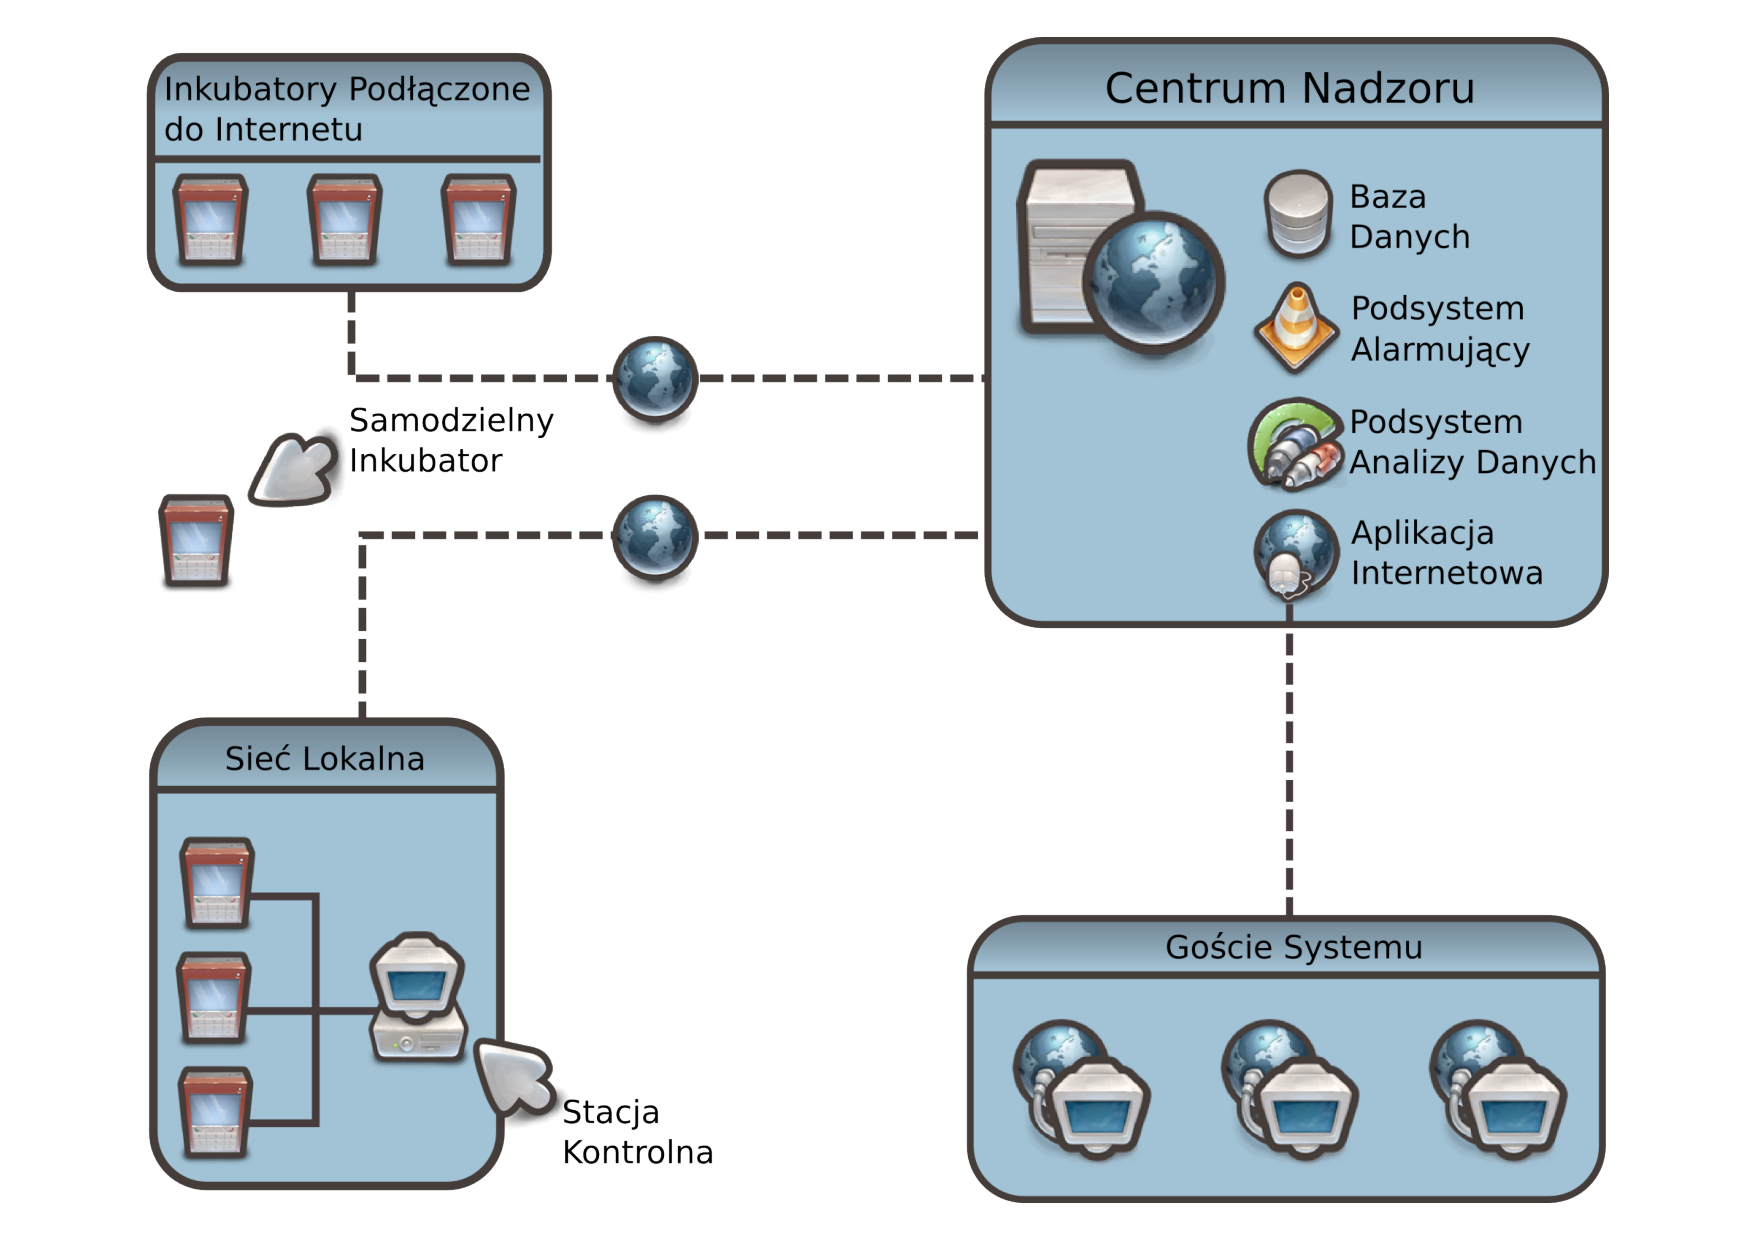
\includegraphics[width=\textwidth]{figures/System_Diagram}
\caption{Diagram systemu}\label{rys:SystemDiagram}
\end{figure}

\paragraph{Poziom 1. -- Inkubator.}
Najważniejszy element systemu. Pozwala na inkubację jaj oraz monitorowanie
tego procesu. Jako samodzielnie urządzenie posiada pełną funkcjonalność typowego
inkubatora. Dodatkowo wyposażony jest w~klawiaturę oraz wyświetlacz LCD,
pozwalające w~intuicyjny sposób programować inkubator oraz wyświetlać aktualne
wartości sterowanych parametrów.

\paragraph{Poziom 2. -- Stacja Kontrolna.}
Komputer połączony z~inkubatorami siecią lokalną Ethernet. Pozwala ornitologom
na zaprogramowanie inkubatora. Pomaga w~doborze optymalnych wartości sterowanych
parametrów w~przypadku jednoczesnej inkubacji jaj różnych gatunków. Na bieżąco
monitoruje i~wizualizuje parametry trwających oraz zakończonych inkubacji.

\paragraph{Poziom 3. -- Centrum Nadzoru.}
Zdalny serwer pracujący non-stop. Składa się z~następujących podsystemów:
\begin{itemize}
	\item bazy danych, która gromadzi informacje o~przebiegu oraz efektywności
		inkubacji ze wszystkich zarejestrowanych w~systemie inkubatorów oraz
		przechowuje wyniki analizy danych,
	\item podsystem alarmowania -- w~równych odstępach czasu rejestruje stan
		wszystkich inkubatorów, a~w~przypadku wykrycia błędnego stanu podejmuje
		odpowiednie działania alarmujące,
	\item podsystem analizy danych -- narzędzia do analizy wpływu warunków
		inkubacji (np. średniej temperatury, najdłuższego czasu bez zasilania) na
		klujność; funkcjonalność ta została zaprojektowana z~myślą o~rozszerzeniu systemu w~przyszłości,
	\item podsystem wizualizacji -- aplikacja internetowa służąca do nadzoru
		systemu i~wizualizacji przechowywanych danych,
	\item podsystem administracyjny -- panel służący do zarządzania inkubatorami.
\end{itemize}

Poszczególne elementy systemu zostały tak zaprojektowane by ściśle
współpracowały z~urządzeniami na niższym poziomie, natomiast były niezależne od
urządzeń na wyższym poziomie. Pozwala to na poprawne działanie systemu
w~przypadku gdy jest on ograniczony do dwóch poziomów (Inkubator i~Stacja
Kontrolna, Inkubator i~Centrum Nadzoru) lub tylko jednego poziomu (Inkubator).
Dodatkowo uniezależnienie poziomów pozwala na zwiększenie niezawodności
systemu oraz zapewnia odporność na utratę danych w~wyniku awarii urządzenia na
niższym poziomie.

\subsection{Zasady działania systemu}
Poniższy scenariusz opisuje ogólny sposób wykorzystania systemu:
\begin{itemize}
	\item Proces inkubacji rozpoczynany jest poprzez umieszczenie w~inkubatorze
		jaj i~zaprogramowanie inkubatora przy pomocy wbudowanej klawiatury lub
		Stacji Kontrolnej. Inkubacja trwa od dwóch tygodni do dwóch miesięcy.
		W~dowolnej chwili można zmienić ustawiony program inkubacji.
	\item Przy programowaniu inkubatora Stacja Kontrolna wyświetla dostępne wzorce
		inkubacji pomagając w~optymalnym doborze sterowanych parametrów.
	\item Stacja Kontrolna regularnie pobiera uaktualnienia wzorców inkubacji
		w~Centrum Nadzoru.
	\item Wartości wszystkich sterowanych parametrów inkubacji są przechowywane
		w~pamięci inkubatora i~mogą być odczytane przez Stację Kontrolną.
	\item Wiadomości kontrolne z~wartościami sterowanych parametrów są wysyłane do
		Stacji Kontrolnej i~Centrum Nadzoru w~równych odstępach czasu.
	\item Ornitolog może sprawdzić stan procesu inkubacji na trzy sposoby (trzy
		poziomy kontroli):
		\begin{itemize}
			\item odczytując wskazania na cyfrowym wyświetlaczu inkubatora,
			\item przy pomocy Stacji Kontrolnej, która wyświetla bieżące wartości
				sterowanych parametrów dla wszystkich działających inkubatorów w~sieci
				lokalnej,
			\item po zalogowaniu do Centrum Nadzoru, do którego ma dostęp z~każdego
				miejsca na świecie.
		\end{itemize}
	\item W~przypadku błędnego stanu inkubacji uruchamiane są trzy sposoby
		alarmowania odpowiadające poziomom kontroli:
		\begin{itemize}
			\item Inkubator -- alarm dźwiękowy,
			\item Stacja Kontrolna -- wyświetlenie powiadomienia,
			\item Centrum Nadzoru -- powiadomienie e-mailowe, możliwość dodania
				funkcjonalności powiadomień sms-owych.
		\end{itemize}
	\item Centrum Nadzoru gromadzi informacje o~przebiegach inkubacji w~celu
		współdzielenia doświadczeń i~analizy danych.
	\item Za przyzwoleniem ogrodu zoologicznego informacja o~stanie inkubatora
		może być udostępniona anonimowym użytkownikom aplikacji internetowej
		w~Centrum Nadzoru. Pozwoli to na zwiększenie zainteresowania użytkowników
		Internetu pracami prowadzonymi w~zoo i~zachęci ich do odwiedzenia ogrodu.
\end{itemize}

\subsection{Opis funkcjonalności systemu}
Poszczególne części systemu thinkubator pełnią następujące funkcje:

\noindent\textbf{Inkubator}:
\begin{itemize}
	\item zapewnienie optymalnych warunków inkubacji poprzez jak najwierniejsze
		odtworzenie rzeczywistych warunków inkubacji,
	\item sterowanie w~zakresie temperatury, wilgotności i~obracania jaj,
	\item wyświetlanie na wyświetlaczu LCD parametrów inkubacji,
	\item możliwość zaprogramowania inkubacji przy pomocy wbudowanej klawiatury,
	\item możliwość zaprogramowania inkubacji przy pomocy Stacji Kontrolnej,
	\item zbieranie danych pomiarowych,
	\item rozsyłanie danych pomiarowych do Stacji Kontrolnej i~Centrum Nadzoru.
\end{itemize}
\textbf{Stacja Kontrolna}:
\begin{itemize}
	\item jednoczesne monitorowanie wszystkich inkubatorów w~sieci,
	\item wizualizacja przebiegu sterowanych parametrów inkubacji w~funkcji czasu
		przez cały okres inkubacji,
	\item programowanie inkubatora,
	\item pomoc w~doborze nastaw poprzez wizualizację wzorców inkubacji jaj
		jednego lub wielu różnych gatunków,
	\item pobieranie uaktualnień wzorców z~Centrum Nadzoru,
	\item przechowywanie danych o~przebiegu inkubacji w~celu wizualizacji lub
		wysłania ich do Centrum Nadzoru.
\end{itemize}
\textbf{Centrum Nadzoru}:
\begin{itemize}
	\item gromadzenie danych z~przebiegu inkubacji (zaprogramowane i~rzeczywiste
		wartości sterowanych parametrów),
	\item monitorowanie bieżącego stanu inkubatorów,
	\item wizualizacja przebiegu wartości sterowanych parametrów dla każdej
		inkubacji,
	\item analiza danych w~celu tworzenia wzorców,
	\item alarmowanie o~błędach,
	\item uwierzytelnianie i~autoryzacja użytkowników -- kontrola dostępu do
		poszczególnych funkcji systemu,
	\item zarządzanie kontami użytkowników.
\end{itemize}

\subsection{Wymagania wydajnościowe}
Mimo szerokiej funkcjonalności systemu Thinkubator, podstawowym wymogiem jakie
musi on spełniać jest zapewnianie odpowiednich warunków inkubacji w~komorze
inkubacyjnej. Inkubator musi zagwarantować sterowanie temperaturą z~dokładnością
przynajmniej~0,3\st{} (optymalnie~0,1\st) oraz wilgotnością z~dokładnością do~5\%
względnej wilgotności (optymalnie~1\%). Komora inkubacyjna powinna pomieścić
około~50 jaj i~być szczelna aby nie dopuszczać do wahań temperatury i~wilgotności.
Wnętrze komory musi być wietrzone by zapewnić świeży dopływ tlenu
oraz nie dopuścić do nadmiernego wzrostu wilgotności. Aby idealnie odwzorowywać
warunki naturalne inkubator musi być wyposażony w~mechanizm obracania jaj.


\chapter{Architektura}
\label{sec:Architektura}

\section{Inkubator}

\subsection{Konstrukcja}
Większość współczesnych inkubatorów ma konstrukcję zewnętrzną polimerową
(np.~z~poliuretanu) albo zbudowaną z~kątowników aluminiowych i~sklejki.
Konstrukcje te są produkowane seryjnie w~profesjonalnych zakładach.
Najczęściej obudowy polimerowe są odlewami. Koszt wykonania takiej formy przekracza
nawet 10~tysięcy~zł. 

Konstrukcję zewnętrzną inkubatora wykonano z~płyty wiórowej, ponieważ jest ona
łatwiejsza w~obróbce niż polimery, natomiast obudowa aluminiowo-sklejkowa jest
droższa i~jej wykonanie jest bardziej czasochłonne (porównywalna konstrukcja
musiałaby się składać z~23~elementów) niż wykonanie obudowy z~płyty wiórowej (7~elementów).
Największą wadą płyty wiórowej jest jej niska odporność na wilgoć. Rozwiązano
ten problem zapewniając szczelność na poziomie polietylenowej konstrukcji
wewnętrznej, która została profesjonalnie zespawana, więc jest w~100\%
hermetyczna. 

Konstrukcja zewnętrzna jest podzielona na dwie części -- inkubacyjną i~techniczną.
W~części inkubacyjnej o~rozmiarze 60~cm~x~50~cm~x~50~cm mieści się
komora inkubacyjna oraz 10-milimetrowa warstwa izolacji styropianowej.
Część techniczna ma rozmiar 20~cm~x~50~cm~x~50~cm i~zawiera przestrzeń na wymiennik
ciepła, silnik oraz system sterowania. 

Konstrukcja wewnętrzna (,,komora inkubacyjna'') jest wykonana z~polietylenu --
bardzo gładkiego i~śliskiego materiału, ułatwiającego mycie i~sterylizację -- to
bardzo istotne dla pracowników ogrodu zoologicznego. Co więcej, polietylen posiada atest na
kontakt z~żywnością, więc jest niegroźny dla piskląt. Komora inkubacyjna
została połączona z~konstrukcją zewnętrzną, aby usztywnić całą konstrukcję
inkubatora. Komora ta wyposażona jest w~dwie ramki o~rozmiarze
43~cm~x~40~cm~x~4~cm, które mogą utrzymać około 50 jaj kurzych. Jej rozmar wynosi 58~cm~x~48~cm~x~48~cm, co zapewnia ramkom odpowiednią przestrzeń, aby
jaja o~wymaganym rozmiarze mogły się obrócić.

Aby odizolować komorę inkubacyjną od konstrukcji zewnętrznej oraz wymiennik
ciepła od reszty części technicznej użyto styropianu. Może on wytrzymać temperaturę rzędu 80\st{} (wymiennik ciepła może
się rozgrzać nawet do 60\st).

% obrazek inkubatora 

\subsection{Projekt mechaniczny}
Obecnie stosuje się dwie technologie obracania jaj:

\begin{itemize}
\item rotacja częściowa - jaja są wkładane pionowo w~specjalne ramki, które utrzymują je
wychylając się pod pewnym kątem. To rozwiązanie jest najczęściej używane
w~inkubatorach jaj strusich (ze względu na ich rozmiar oraz na cechy gatunku)
oraz w~inkubatorach drobiu na skalę przemysłową (ze względu na małą utratę
miejsca w~inkubatorze);

\item rełna rotacja - jaja są wkładane poziomo na rolki obracające się o~180\st{} w~przeciwnych
kierunkach. To~rozwiązanie jest trudniejsze w~konstrukcji oraz wymaga
dodatkowego miejsca, gdyż w~większości implementacji tego rozwiązania rolki z~jajami
przemieszczają się w~poziomie. Z~drugiej strony uważa się, że~to rozwiązanie daje większą
szansę na sukces podczas inkubacji.
\end{itemize}
W~Inkubatorze wybrano mechanizm pełnej rotacji, ze względu na to, że~celem projektu jest
maksymalizacja prawdopodobieństwa sukcesu podczas inkubacji -- każde pisklę może
się okazać bezcenne.
 
Główną częścią systemu rotacyjnego jest silnik elektryczny z~mechanizmem
samopowrotowym (w~momencie, gdy napotka opór zmienia kierunek ruchu).
Silnik napędza śrubę trapezową o~skoku 4~mm z~trzema nakrętkami -- jedną ,,napędową''
oraz dwoma ,,blokującymi''. Nakrętka ,,napędowa'' połączona jest
z~ramkami za pomocą płaskownika aluminiowego natomiast nakrętki ,,blokujące'' 
nakręcone są w~miejscu gdzie mechanizm rotacji ma zawrócić (połowa obwodu
inkubowanych jaj). W~momencie gdy nakrętka napędowa połączy się z~blokującymi,
silnik odbija i~śruba zaczyna się kręcić w~przeciwną stronę.

Do~inkubatora załączonych jest dwadzieścia rolek, które można zamocować w~ramkach
idealnie dopasowując odległość między nimi do rozmiarów inkubowanych jaj. Model
ramek z~rolkami przedstawiony jest na rysunku~\ref{rys:rolki}.

\begin{figure}[t] 
	\centering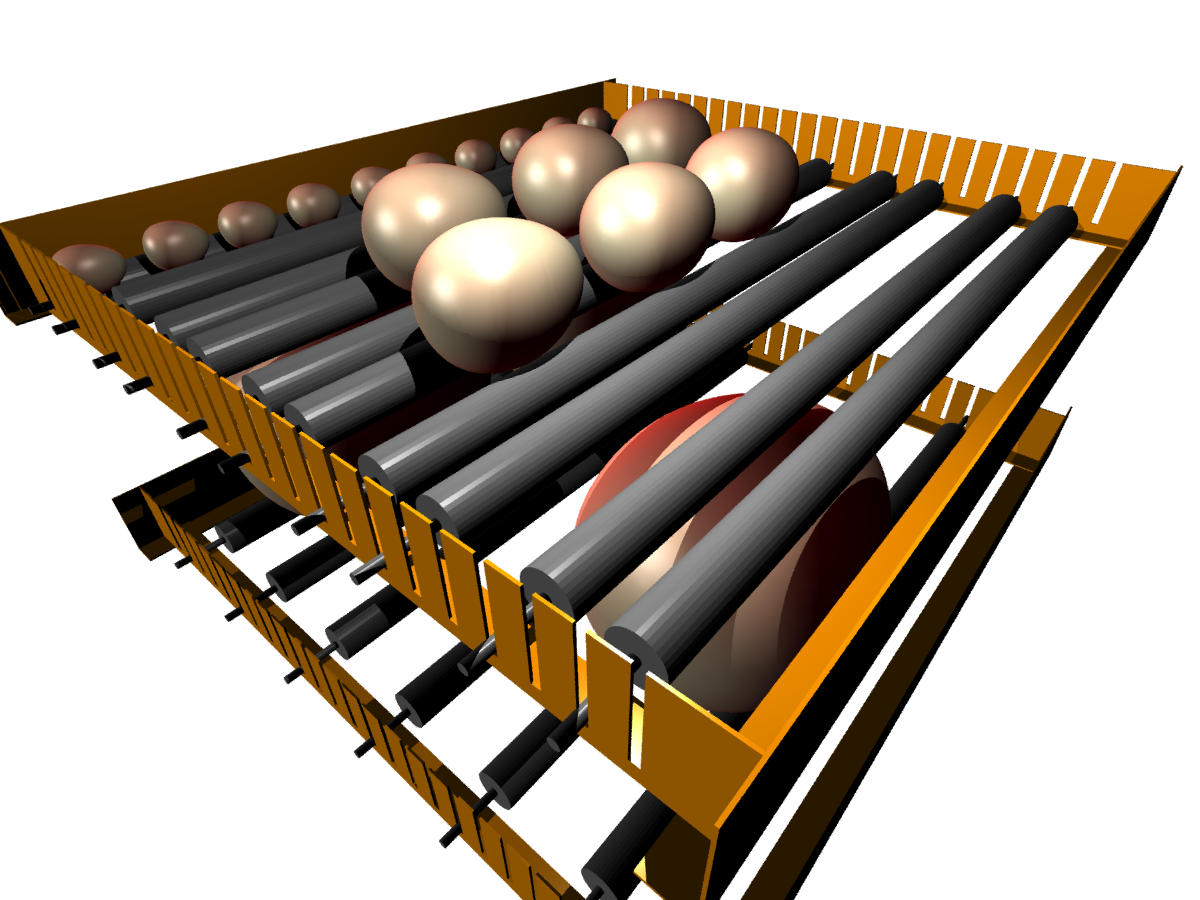
\includegraphics[width=\textwidth]{figures/rolki}
	\caption{Model ramek z~rolkami}\label{rys:rolki}
\end{figure}

\subsection{Wymiennik ciepła}
Sterowanie temperaturą z~dokładnością dochodzącą do $0,1$\st{} jest bardzo
trudnym zadaniem, dlatego potrzebny jest dobry system urządzeń wykonawczych.
Obecnie stosuje się trzy typy rozwiązań:
\begin{itemize}
	\item bezpośrednie podgrzewanie powietrza przez grzałki zainstalowane w~podłodze, 
	\item płaszcz wodny -- podgrzewanie wody otaczającej komorę inkubacyjną --
		rozwiązanie bardzo trudne w~wykonaniu (2 szczelne warstwy, wymuszanie ruchu
		wody na tym obszarze), lecz daje się dość dobrze nim sterować,
	\item podgrzewanie powietrza poza komorą inkubacyjną -- dość łatwe w~wykonaniu
		i~sterowaniu; trudność konstrukcyjna polega na odpowiednim pobraniu
		powietrza z~komory inkubacyjnej i~wprowadzeniu go z~powrotem tak,
		by zapewnić równomierne wymieszanie powietrza w~komorze. 
\end{itemize}

W~Inkubatorze wybrany został system ogrzewania powietrza poza komorą w~tzw. wymienniku ciepła, ponieważ minimalizuje on niepożądany wpływ 
elementów sterujących na obiekt sterowany i~upraszcza modelowanie. Przepływ powietrza z~komory inkubacyjnej przez wymiennik wymuszany jest przez wentylator o~mocy 20W. Jako element grzejny zastosowano suszarkę do włosów, ze względu na jej doskonałe parametry -- moc 1000 W~i praktycznie zerową inercję. Pozwala ona na bardzo szybkie oddziaływanie na temperaturę powietrza w~Inkubatorze. Dodatkowym atutem 
suszarki jest zintegrowany z~nią wentylator. Zapewnia on odpowiedni ruch powietrza podczas grzania, zapobiegając przegrzaniu wymiennika ciepła. 
% *~obrazek górnej części wymiennika -- 

Podczas fazy projektowania Inkubatora rozpatrzono kilka systemów sterowania
wilgotnością. Te najczęściej spotykane w~komercyjnych rozwiązaniach to:
\begin{itemize}
	\item wanna z~otwartą wodą, gdzie osobno ogrzewana jest woda, a~osobno
		pomieszczenie,
	\item grzałka o~dużej inercji na którą kapie woda,
	\item ,,wstrzykiwanie pary'' (\english{direct steam injection}).
\end{itemize}
Po konsultacji z~pracownikami Zoo systemy te okazały się jednak niewystarczające,
ponieważ nie są w~stanie wygenerować wystarczająco wysokiej wilgotności, a~sam
proces nawilżania powietrza znacząco wpływa na temperaturę powietrza wewnątrz
komory. 

Problemy przedstawione powyżej oraz poszukiwania w~Internecie zaowocowały
zastosowaniem nawilżacza ultradźwiękowego. Jego niesamowita wydajność dochodząca
do 200 ml wody wprowadzonych do powietrza w~ciągu godziny, przy zachowaniu
niskiego poboru mocy (20 wat) była najlepszym potwierdzeniem słuszności tego wyboru.

% -- obrazek dolnej części wymiennika --

Grzałka i~nawilżacz umieszczone są we wspólnym układzie, w~taki sposób by 
nawilżać świeżo ogrzane powietrze, które bardziej chłonie wilgoć. 
Model wymiennika ciepła przedstawiony jest na rysunku~\ref{rys:Wymiennik}.

\begin{figure}[b] 
	\centering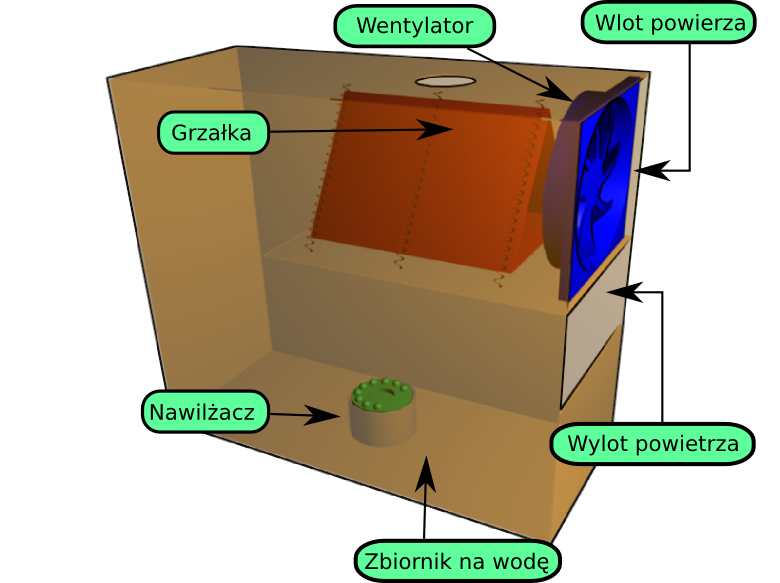
\includegraphics[width=0.9\textwidth]{figures/Wymiennik}
	\caption{Wymiennik ciepła}\label{rys:Wymiennik}
\end{figure}


% -- RURY
\subsection{Model}
Na potrzeby konkursu \emph{CSIDC} stworzono trójwymiarowy model Inkubatora, na
którym wzorowano się później przy jego konstrukcji. Końcowy wygląd urządzenia jest
bardzo zbliżony do tego przedstawionego na rysunku \ref{rys:InkubatorModel},
w~którym jednocześnie zawarto opisy najważniejszych części, co pomaga w~ich
odnalezieniu w~samym urządzeniu.

\begin{figure}[t] 
	\centering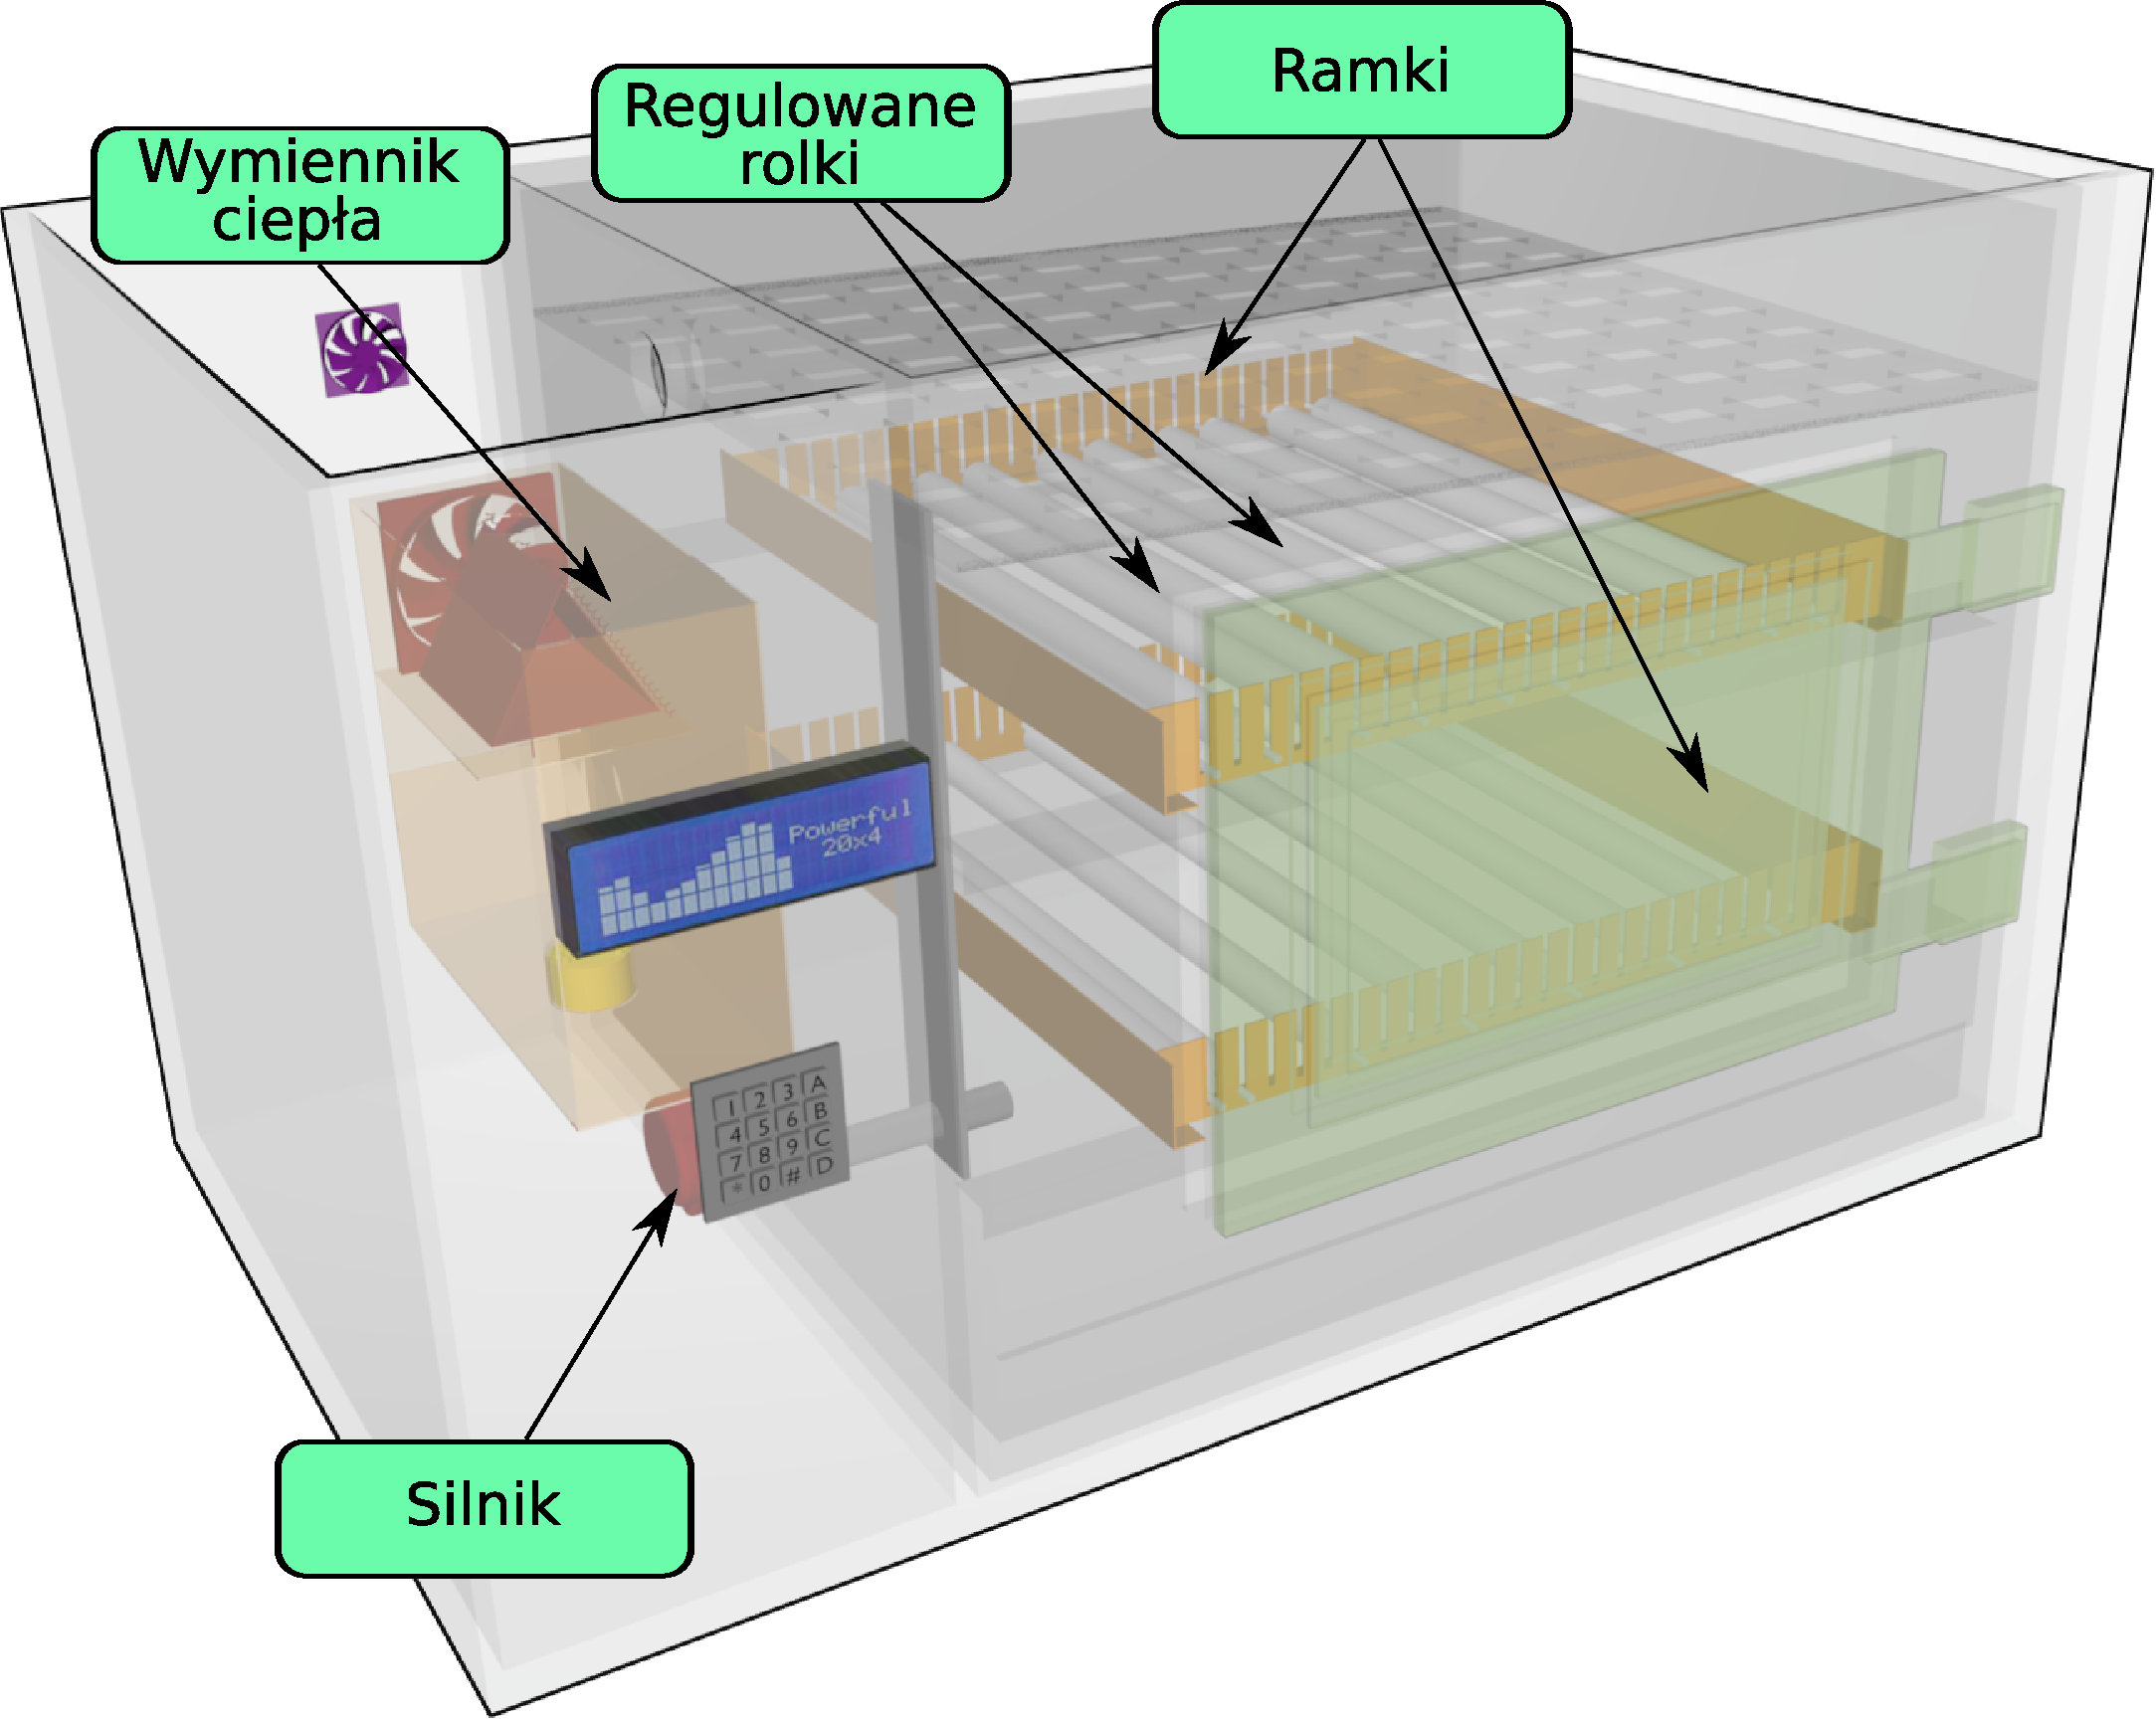
\includegraphics[width=\textwidth]{figures/Incubator}
	\caption{Model inkubatora}\label{rys:InkubatorModel}
\end{figure}

\subsection{Algorytm sterowania}
Celem algorytmu sterowania jest utrzymanie w~komorze inkubacyjnej zadanej
wartości temperatury oraz wilgotności. Do oceny jakości algorytmu sterowania
użyto średniej oraz maksymalnej wartości uchybu regulacji. Według ekspertów doskonały
inkubator powinien popełniać błąd mniejszy niż 0,1\st{} przy sterowaniu
temperaturą oraz błąd mniejszy niż 1\% przy sterowaniu wilgotnością.

Inkubator można zamodelować jako układ zamknięty ze sprzężeniem zwrotnym
\cite{Brzozka04} \cite{Bubnicki}
przedstawiony na rysunku \ref{rys:DiagramSterowania}. Bardziej szczegółowy
schemat układu ukazuje rysunek \ref{rys:SchematLogiczny}.

\begin{figure}[t] 
	\centering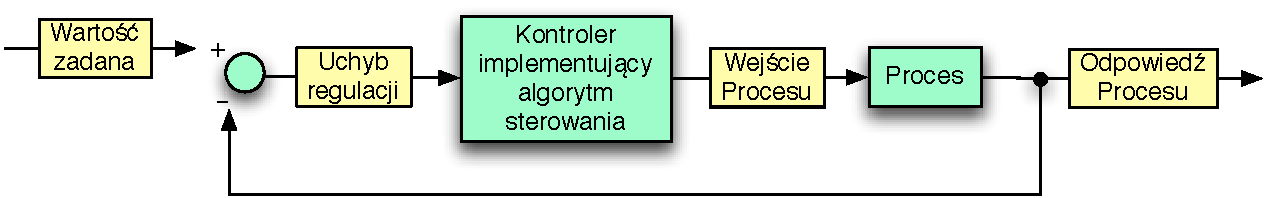
\includegraphics[width=\textwidth]{figures/DiagramSterowania}
	\caption{Układ regulacji z~logiką rozmytą}\label{rys:DiagramSterowania}
\end{figure}
	
\begin{figure}[t] 
	\centering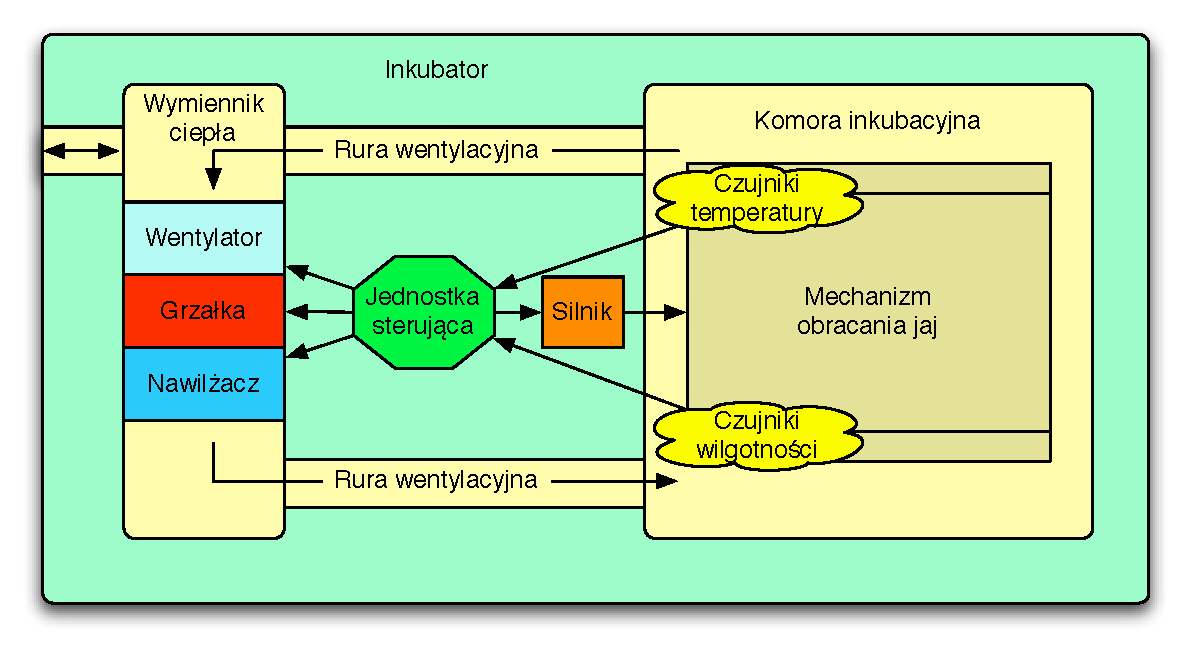
\includegraphics[width=\textwidth]{figures/SchematLogiczny}
	\caption{Schmat inkubatora}\label{rys:SchematLogiczny}
\end{figure}
	
W~fazie testowania sprzętu został zastosowany domyślny algorytm sterowania --
załącz/wyłącz. Algorytm ten dał doskonałe rezultaty przy sterowaniu wilgotnością
(dokładność 1\%) oraz przeciętne rezultaty przy sterowaniu temperaturą
(dokładność 0,8\st).

Proces jednoczesnego sterowania wilgotnością i~temperaturą jest bardzo
skomplikowany, ponieważ obie funkcje wykazują pewną korelację (np. wzrost
temperatury obniża względną wilgotność). W~przypadku inkubatora istnieją jednak
następujące podstawy by pominąć tę zależność:
\begin{itemize}
	\item przez cały czas zarówno temperatura jak i~wilgotność utrzymywane są na stałym poziomie, minimalne odchylenia jednego parametru nie mają istotnego wpływu na wartość drugiego,
	\item niezależne sterowanie temperaturą i~wilgotnością pozwala na znaczne uproszczenie modelu oraz napisanie czytelniejszego, łatwiejszego w~modyfikacji i~bardziej niezawodnego algorytmu.
\end{itemize}

Zastosowany algorytm sterowania wzorowany był na logice rozmytej \cite{FuzzyLogic} \cite{Piegat}. Wybrany został
algorytm logiki rozmytej ze względu na cechy przydatne w~zastosowaniu:
\begin{itemize}
	\item brak konieczności znajomości modelu matematycznego procesu,
	\item łatwość reprezentacji,
	\item wysoka potwierdzona doświadczalnie dokładność.
\end{itemize}

Parametrem wejściowym algorytmu sterowania jest wartość uchybu regulacji $e$
oraz jego pierwsza pochodna $\dot{e}$. Wyjście algorytmu określa sposób oddziaływania
$y =~f(e,\dot{e})$. 
%[[Dla wartości wejściowych oraz wyjściowych zdefiniowano trzy zbiory rozmyte:
%$negatywny$, $zerowy$, $pozytywny$.]]
Funkcja $f(e,\dot{e})$ jest skonstruowana jako suma ważona decyzji podejmowanej na
podstawie wartości uchybu $y_1 =~f_1(e)$ i~decyzji podejmowanej na podstawie
wartości pierwszej pochodnej uchybu $y_2 =~f_2(\dot{e})$. Funkcje $f_1$, $f_2$ mają
postać nierosnących liniowych funkcji sklejanych. Przyjmują one wartości
z~przedziału $[-1, 1]$, gdzie wartość $-1$ oznacza oddziaływanie ujemne, $0$ -- brak
oddziaływania zaś $1$ -- oddziaływanie dodatnie.
%[[maksymalną przynależność do zbioru $negatywny$, $0$ -~$zerowy$ zaś $1$ -
%$pozytywny$.]]
Intuicja podpowiada by większy wpływ na decyzję o~oddziaływaniu miała wartość
uchybu regulacji, zaś w~przypadku gdy wartość ta nie jest rozstrzygająca (czyli
bliska zeru), do głosu była dopuszczana wartość pochodnej. Zgodnie z~tym
podejściem funkcja $f(e,\dot{e})$ została zdefiniowana następująco:
\begin{equation}
f(e,\dot{e}) =~f_1(e) +~(1-|f_1(e)|) \cdot f_2(\dot{e}).
\end{equation}
Decyzja podejmowana na podstawie pochodnej uchybu $\dot{e}$ ma tym większą wagę im
mniejszą (co do wartości bezwzględnej) wartość ma funkcja $f_1$. Początkowo
przebieg funkcji sklejanych $f_1$ i~$f_2$ został ustalony arbitralnie. Algorytm
sterowania temperaturą dawał wówczas dokładność sterowania rzędu 0,5\st. Wynik
ten był lepszy od wyniku algorytmu załącz/wyłącz, co potwierdziło użyteczność
przyjętego algorytmu. Seria dalszych eksperymentów pozwoliła na taki dobór
funkcji $f_1$ i~$f_2$, by błąd sterowania temperaturą mieścił się w~granicach
0,1\st. Wynik ten jest najlepszym z~wyników możliwych do osiągnięcia, zwłaszcza że wartość
0,1 stanowi maksimum uchybu regulacji, zaś średni uchyb jest niemalże równy
zeru. Ostateczną postać liniowych funkcji sklejanych $y_1 =~f_1(e)$
i~$y_2~=f2(\dot{e})$, uzyskanych drogą empiryczną przedstawiają
rysunki~\ref{rys:t_zygzaczek} i~\ref{rys:dt_zygzaczek}.

%[[wektor ma zrobić wykresy liniowych funkcji sklejanych]]

\begin{figure}[p] 
	\centering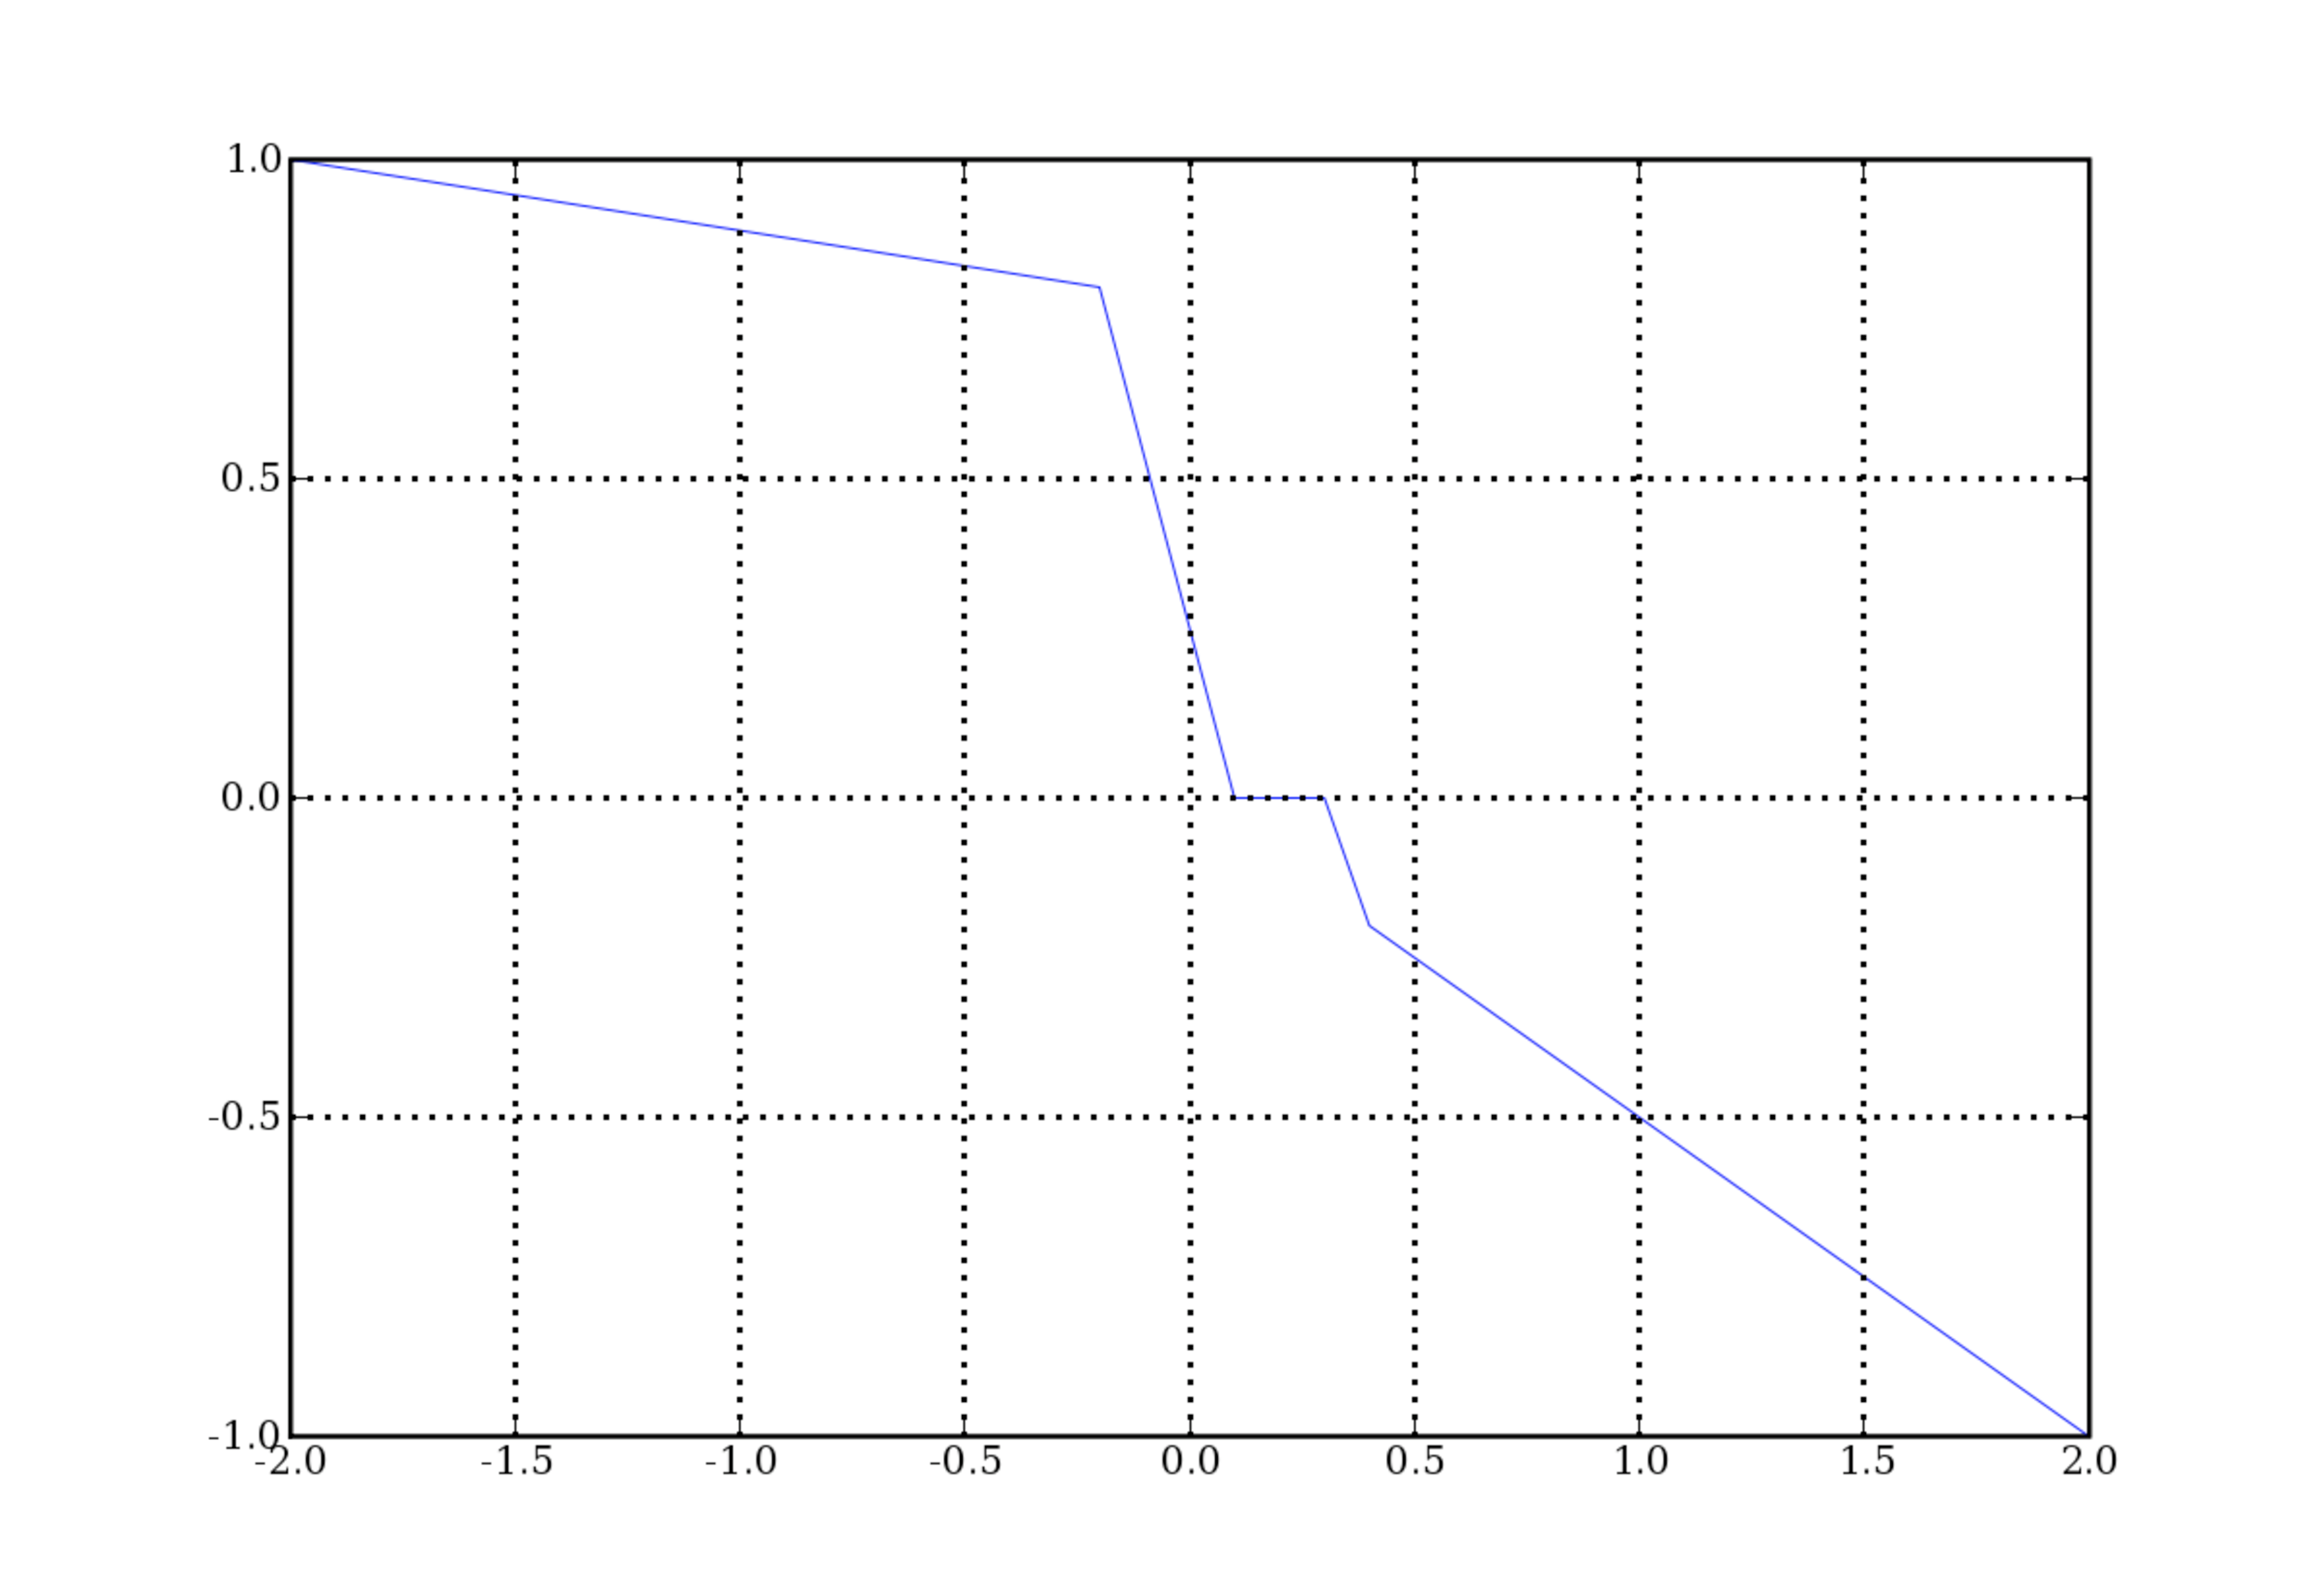
\includegraphics[width=\textwidth]{figures/t_zygzaczek}
	\caption{Odpowiedź względem temperatury ($f_1(e)$)}\label{rys:t_zygzaczek}
\end{figure}

\begin{figure}[p] 
	\centering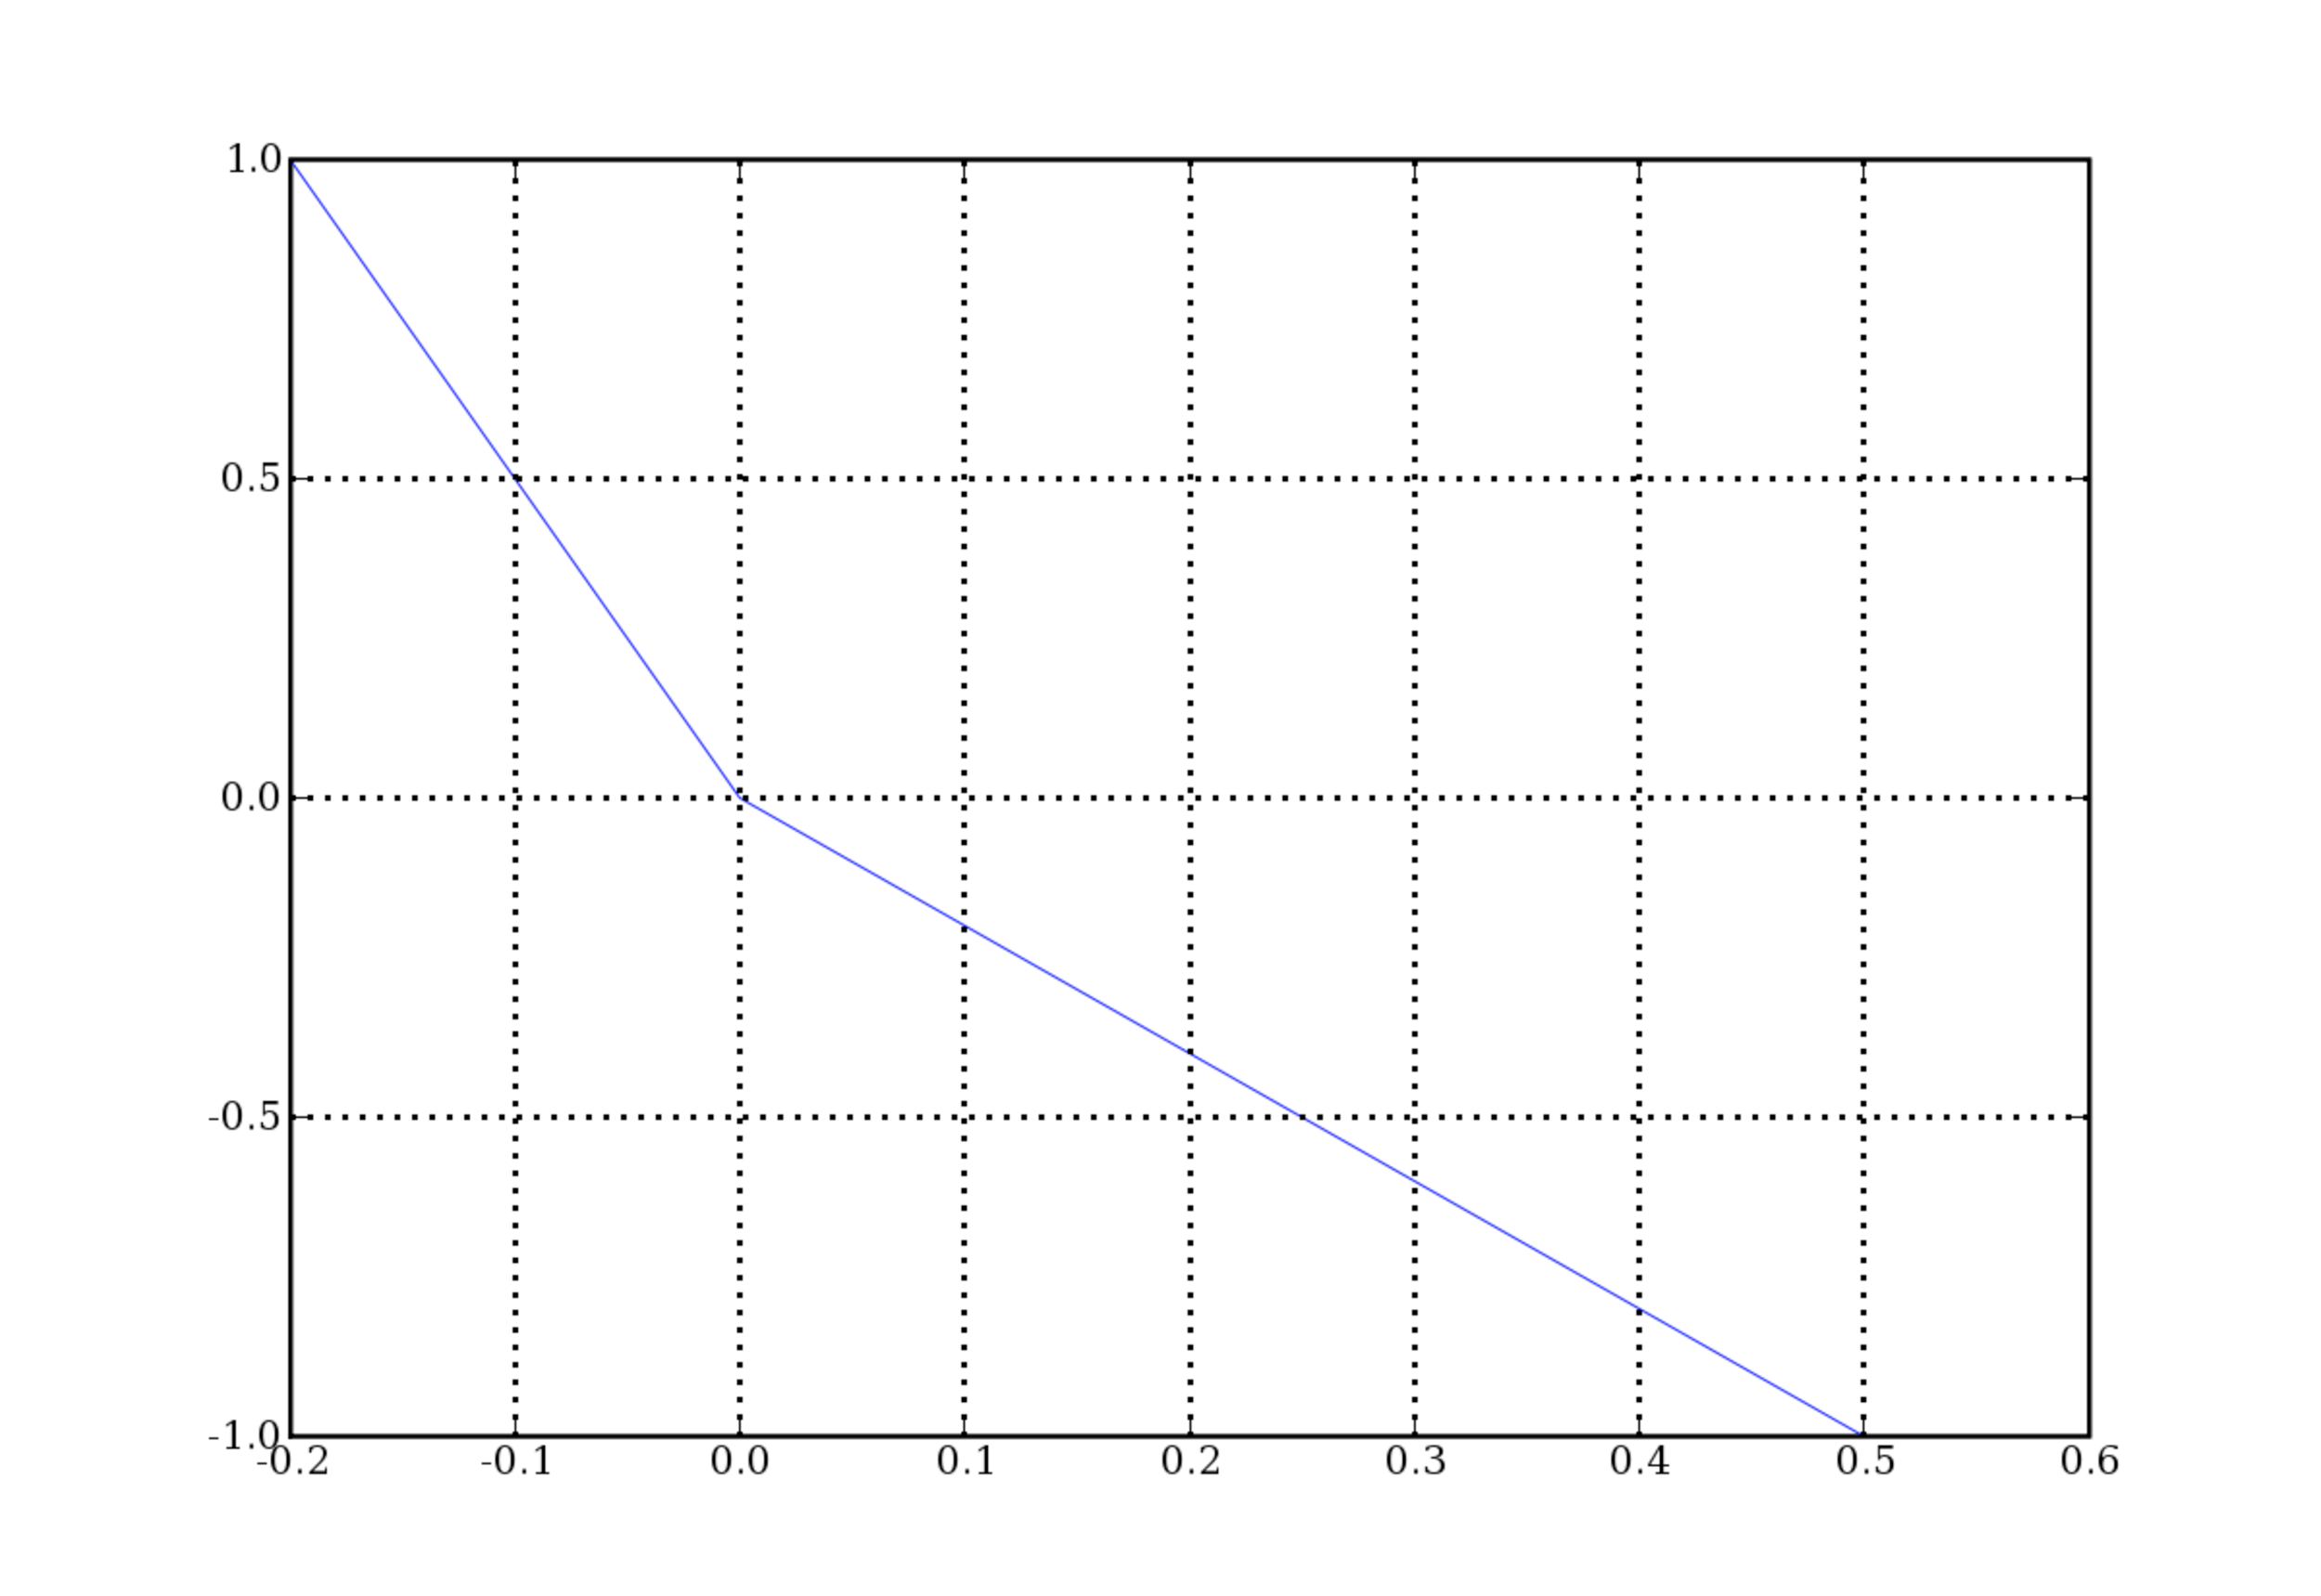
\includegraphics[width=\textwidth]{figures/dt_zygzaczek}
	\caption{Odpowiedź względem zmiany temperatury ($f_2(\dot{e})$)}\label{rys:dt_zygzaczek}
\end{figure}

Odpowiedź algorytmu w~całej dziedzinie argumentów przedstawiona jest
na rysunku \ref{rys:sterowanie3d}.

\begin{figure}[t] 
	\centering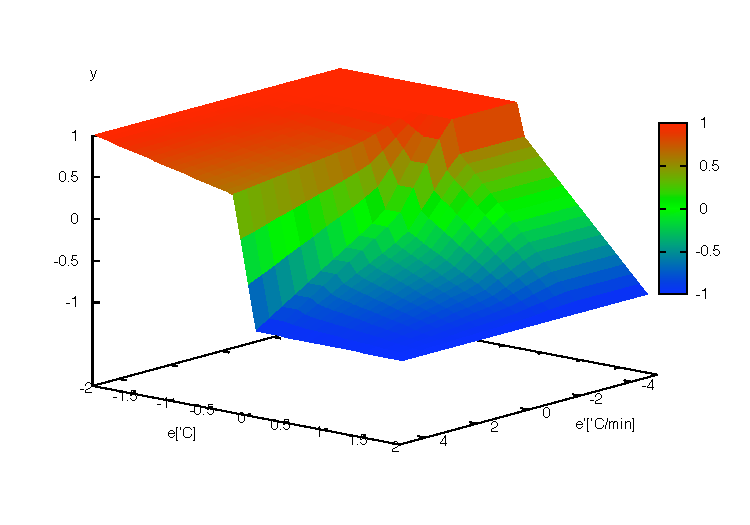
\includegraphics[width=16cm]{figures/sterowanie3d}
	\caption{Odpowiedź w~całej dziedzinie, rzut 3d ($f(e, \dot{e})$)}\label{rys:sterowanie3d}
\end{figure}

Opisany algorytm został zastosowany do sterowania temperaturą, natomiast do
sterowania wilgotnością wykorzystano sprawdzony wcześniej algorytm załącz/wyłącz.
W implementacji oba algorytmy rejestrują wartości uchybów co $w$ sekund oraz
podejmują decyzję co $n \cdot w$ sekund. Wartość uchybu ($e$) wykorzystywana na wejściu
algorytmu sterowania obliczana jest jako średnia z~ostatnich trzech zmierzonych
uchybów, wartość pochodnej uchybu ($\dot{e}$) jest obliczana jako różnica między
średnią z~trzech ostatnich uchybów i~średnią z~trzech poprzednich uchybów.

\subsection{Elektronika}
Prawidłowy przebieg inkubacji zapewnia komputer pokładowy. Spełnia on poniższe wymagania:
\paragraph{Niezawodność.} 
Po przeprowadzeniu rozpoznania wybrano komputer PCM-9575 produkowany przez firmę
Advantech. Jest to tzw. ,,Single Board Computer'' formatu EBX 5,25 cala
z~procesorem VIA Embedded Eden 400MHz, którego wydajność w~zupełności wystarcza.
Komputer ten może działać bez wentylatora w~temperaturach do 60\st, co pozwala
działać mu bezawaryjnie w~warunkach wewnątrz inkubatora. Wbudowany interfejs
VGA/LCD pozwala podłączyć monitor i~bezpośrednio obserwować działanie algorytmów
i~stan procesów, a~także wprowadzać poprawki w~sposób interaktywny.

\paragraph{Wysoka wydajność.}
Uruchomienie wielu osobnych procesów wymaga odpowiedniej mocy obliczeniowej oraz
odpowiedniej ilości pamięci RAM. Procesor ma zapas mocy która może okazać się
potrzebna w~przypadku wprowadzenia dodatkowej funkcjonalności. Rozmiar pamięci
operacyjnej -- 128 MB jest szczególnie istotny, ponieważ w~trakcie działania
aplikacji większość operacji odczytu i~zapisu przeprowadzanych jest na
wirtualnym systemie plików właśnie w~pamięci operacyjnej, celem zminimalizowania
liczby operacji odczytu i~zapisu na karcie pamięci CompactFlash.

\paragraph{Minimalny koszt wdrożenia.}
W celu obniżenia kosztu wdrożenia Thinkubatora do ogrodów zoologicznych
zadecydowano o~użyciu połączeń ethernetowych. Polskie ogrody są już podłączone do
internetowego systemu inwentaryzowania zwierząt ISIS (\emph{http://www.isis.org}),
zatem infrastruktura sieciowa jest gotowa do użycia.

\paragraph{Rozszerzalność.}
Thinkubator znajduje się obecnie na etapie prototypu. Możliwość podłączenia
dysków EIDE lub urządzeń USB umożliwia rozszerzanie systemu o~standardowe
komponenty. Korzystając z~interfejsu PC/104-Plus komputer pokładowy można
dowolnie rozszerzać o~specjalistyczne urządzenia, które mogą mieć zastosowanie
w~ogrodach zoologicznych ze specjalnymi wymaganiami.

\paragraph{Łatwość rozwijania.}
Komputer posiada wbudowany czytnik kart typu CompactFlash. Na przygotowanej karcie CompactFlash
o~pojemności 256MB znajduje się system i~pliki konfiguracyjne, a~także partycja
służąca za nieulotną pamięć do zapisu. Gdy połączenie Ethernet jest niedostępne,
historia inkubacji jest zapisywana na karcie, którą można następnie odczytać na
zwykłym komputerze PC i~przesłać do Centrum Nadzoru.

Sterowanie środowiskiem opera się na sprzężeniu zwrotnym. Zastosowano kilka
rodzajów czujników. Do pomiaru wilgotności zdecydowano się na użycie
zintegrowanego czujnika wilgotności i~temperatury Dallas Hygrochron ze względu
na jego wysoką precyzję (0,6\%RH) oraz możliwość łatwej komunikacji cyfrowej. Do
produkcji seryjnej przewiduje się dużo tańsze czujniki pojemnościowe, jednak dla
celów przejrzystości w~prototypie stosowano rozwiązania pewne i~sprawdzone.
Pomiary przekazywane są poprzez magistralę szeregową 1-wire.

Do tej samej magistrali podłączono trzy czujniki temperatury serii DS1820.
Zastosowanie tradycyjnego termostatu było wykluczone ze względu na konieczność
centralnego sterowania środowiskiem z~komputera. Zmierzona wartość temperatury
wyświetlana jest na ekranie ciekłokrystalicznym. Eliminuje to konieczność
umieszczenia termometru rtęciowego w~komorze inkubacyjnej i~wiążącego się z~tym
zagrożenia zatruciem tlenkami rtęci w~przypadku uszkodzenia.

Czujniki podłączone są do opracowanej przez Dallas Semiconductors szyny 1-wire.
Używa ona jedynie dwóch przewodów, jednego do zasilania i~przesyłania sygnałów,
drugiego do masy, dzięki czemu jest bardzo łatwa we wprowadzeniu i~rozbudowie.
Można do niej podłączyć dużą liczbę różnych urządzeń, m.in. czujników,
adresowalnych przełączników, potencjometrów cyfrowych. W~Inkubatorze
wykorzystano samodzielnie zbudowany adapter podłączany do portu RS-232. 
Schemat ideowy adaptera widoczny jest na rysunku \ref{rys:Adapter}.

\begin{figure}[t] 
\centering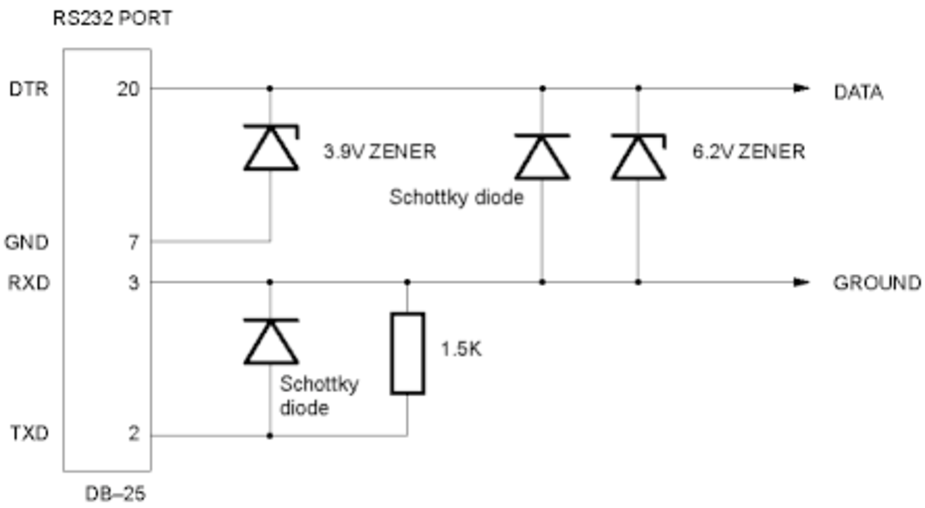
\includegraphics[width=\textwidth]{figures/adapter}
\caption{Adapter 1-wire}\label{rys:Adapter}
\end{figure}

Interfejs użytkownika inkubatora składa się z~niebiesko-białego wyświetlacza
ciekłokrystalicznego zawierającego po 20 znaków w~2 rzędach
oraz klawiatury z~16 guzikami podłączonej do portu \emph{PS/2}. Ekran podłączony
jest do portu równoległego komputera w~trybie 4-bitowym.

Sygnały z~komputera są wyprowadzone poprzez port równoległy. Oświetlenie komory
lęgowej wykonano przy użyciu diod LED, zapewniając wysoką trwałość systemu
oświetlenia i~umożliwiając nieskrępowane załączanie i~wyłączanie oświetlenia bez
wprowadzania wahań temperatury. Diody są załączane poprzez tranzystor, natomiast trzy
urządzenia wykonawcze są włączane przez płytkę z~przekaźnikami.

Grzałka na 230V jest podłączona do przekaźnika, który załącza napięcie w~odpowiednim momencie.

Nawilżacz jest również załączany poprzez przekaźnik. Potrzebny mu zasilacz 24V
prądu zmiennego jest podłączony do wejścia 220V wewnątrz części technicznej inkubatora.

Silnik do przesuwania rolek jest podłączony do źródła napięcia 220V
i~uruchamiany za pomocą przekaźnika.

\subsection{Aplikacja sterująca}
Architektura aplikacji sterującej inkubatorem oparta jest na grupie niezależnych
procesów komunikujących się ze sobą za pomocą segmentu pamięci współdzielonej.
Procesy zostały zaprojektowane w~taki sposób, aby nie nie wymagały silnego
zarządzania współbieżnością, ponieważ każdy z~nich wykonuje własne unikatowe
operacje. Interakcje pomiędzy procesami zostały przedstawione na rysunku
\ref{rys:SHM}.

\begin{figure}[t] 
\centering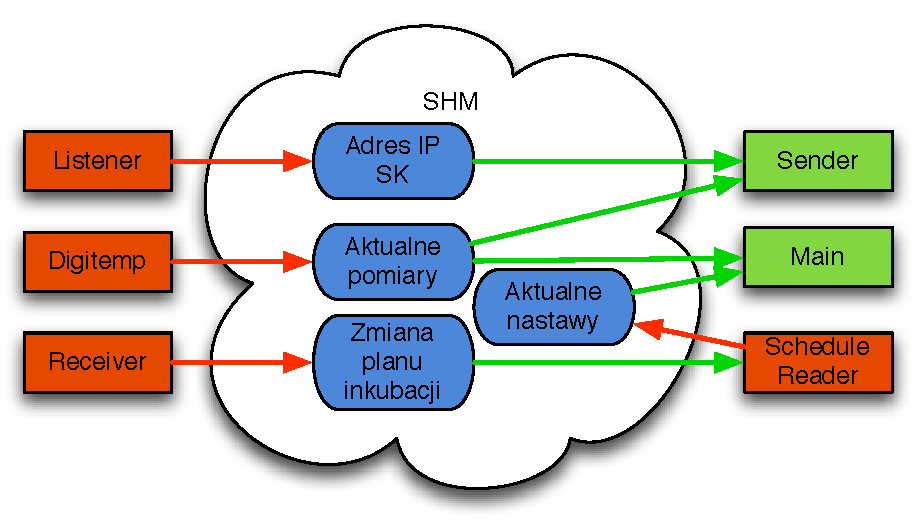
\includegraphics[width=\textwidth]{figures/SHM}
\caption{Schemat procesów}\label{rys:SHM}
\end{figure}

Proces \textbf{Main} jest najważniejszą częścią aplikacji. Korzysta
z~wszystkich informacji zbieranych przez inne procesy i~na ich podstawie podejmuje
decyzje o~uruchamianiu odpowiednich urządzeń wykonawczych w~celu najlepszego
odwzorowania planu inkubacji wewnątrz inkubatora. Jest podzielony na dwie główne
części: moduł abstrakcji sprzętowej, czyli zaimplementowane funkcje włączające
i~wyłączające urządzenia oraz algorytm sterowania, który do poprawnego działania
potrzebuje dwóch informacji. Pierwszą są aktualne parametry komory inkubacyjnej
-- temperatura i~wilgotność, za zbieranie których odpowiedzialny jest proces
\textbf{Digitemp} -- adaptacja otwartego programu o~tej samej nazwie służącego
do odczytywania informacji z~czujników 1-wire; drugą -- parametry inkubacji
nastawione przez operatora urządzenia. Dostarcza je proces \textbf{Schedule
Reader}, którego zadaniem jest także wczytywanie nowego planu inkubacji, jeśli ten
zostanie zmieniony w~trakcie jej trwania. \textbf{Sender} jest odpowiedzialny za
cykliczne wysyłanie informacji na temat stanu inkubacji do \emph{Stacji
Kontrolnej} oraz \emph{Centrum Nadzoru}, natomiast \textbf{Receiver} nasłuchuje
ruch sieciowy i~odpowiada na wszystkie wiadomości wysłane do inkubatora za
wyjątkiem sygnału rozgłoszeniowego wyszukującego inkubatory -- za tę czynność
odpowiedzialny jest \textbf{Listener}.

Dodatkowo działają dwa procesy związane z~interfejsem zamontowanym na
inkubatorze -- wyświetlaczem LCD oraz klawiaturą. 

Proces keyboardd oczekuje na sygnały z~klawiatury. Wykorzystywana jest metoda
"poll". Poprzez załączanie napięcia na kolejnych liniach szyny poziomej
i~odczytywanie stanu poszczególnych linii szyny pionowej otrzymujemy bieżący stan
klawiatury. Po zmianie stanu jednej z~odczytywanych linii na wysoki i~powrotu do
stanu niskiego wprowadzony znak jest rozpoznawany i~umieszczany w~kolejce FIFO
/dev/kbd.

Proces displayd prezentuje na wyświetlaczu LCD przede wszystkim bieżący stan
środowiska wewnątrz inkubatora. W~przypadku problemów wyświetla informacje
o~zaistniałym zagrożeniu i~podaje źródło, z~którego można zasięgnąć informacji
które będą służyły rozwiązaniu problemu. Ekran ciekłokrystaliczny stanowi też ważny
komponent systemu sterowania inkubatorem: wyświetla złożony system menu,
pozwalający na konfigurację, zaawansowany monitoring oraz wykonywanie
czynności serwisowych.

Przez większość czasu proces oczekuje na operację odczytu z~kolejki FIFO.
Jednocześnie program wykorzystuje mechanizm sygnałów, aby obsłużyć zdarzenia z~innych
źródeł. Przykładowo, czas na zaktualizowanie wyświetlanej temperatury jest
sygnalizowany co sekundę poprzez dostarczenie SIGALRM zamówionego przy pomocy
funkcji systemowej alarm. Po nadejściu sygnału (czas zaktualizowania
wyświetlanej temperatury, otwarcie drzwiczek, itd.) program przechodzi do jego
obsługi i~wraca oczekiwać na nowy znak. Przez cały ten czas na wyświetlaczu
widać bieżącą temperaturę i~wilgotność lub bieżący wycinek systemu menu -- listę
opcji, zachętę do wprowadzenia nowej temperatury czy potwierdzenie operacji
wyłączenia inkubatora.

Diagram przejść stanów programu obsługi wyświetlacza znajduje się na
rysunku~\ref{rys:Menu}. Przedstawia on zaimplementowany schemat menu, jego
strukturę oraz działanie. Stanowi równocześnie ważną część instrukcji obsługi
inkubatora.


\begin{figure}[b] 
\centering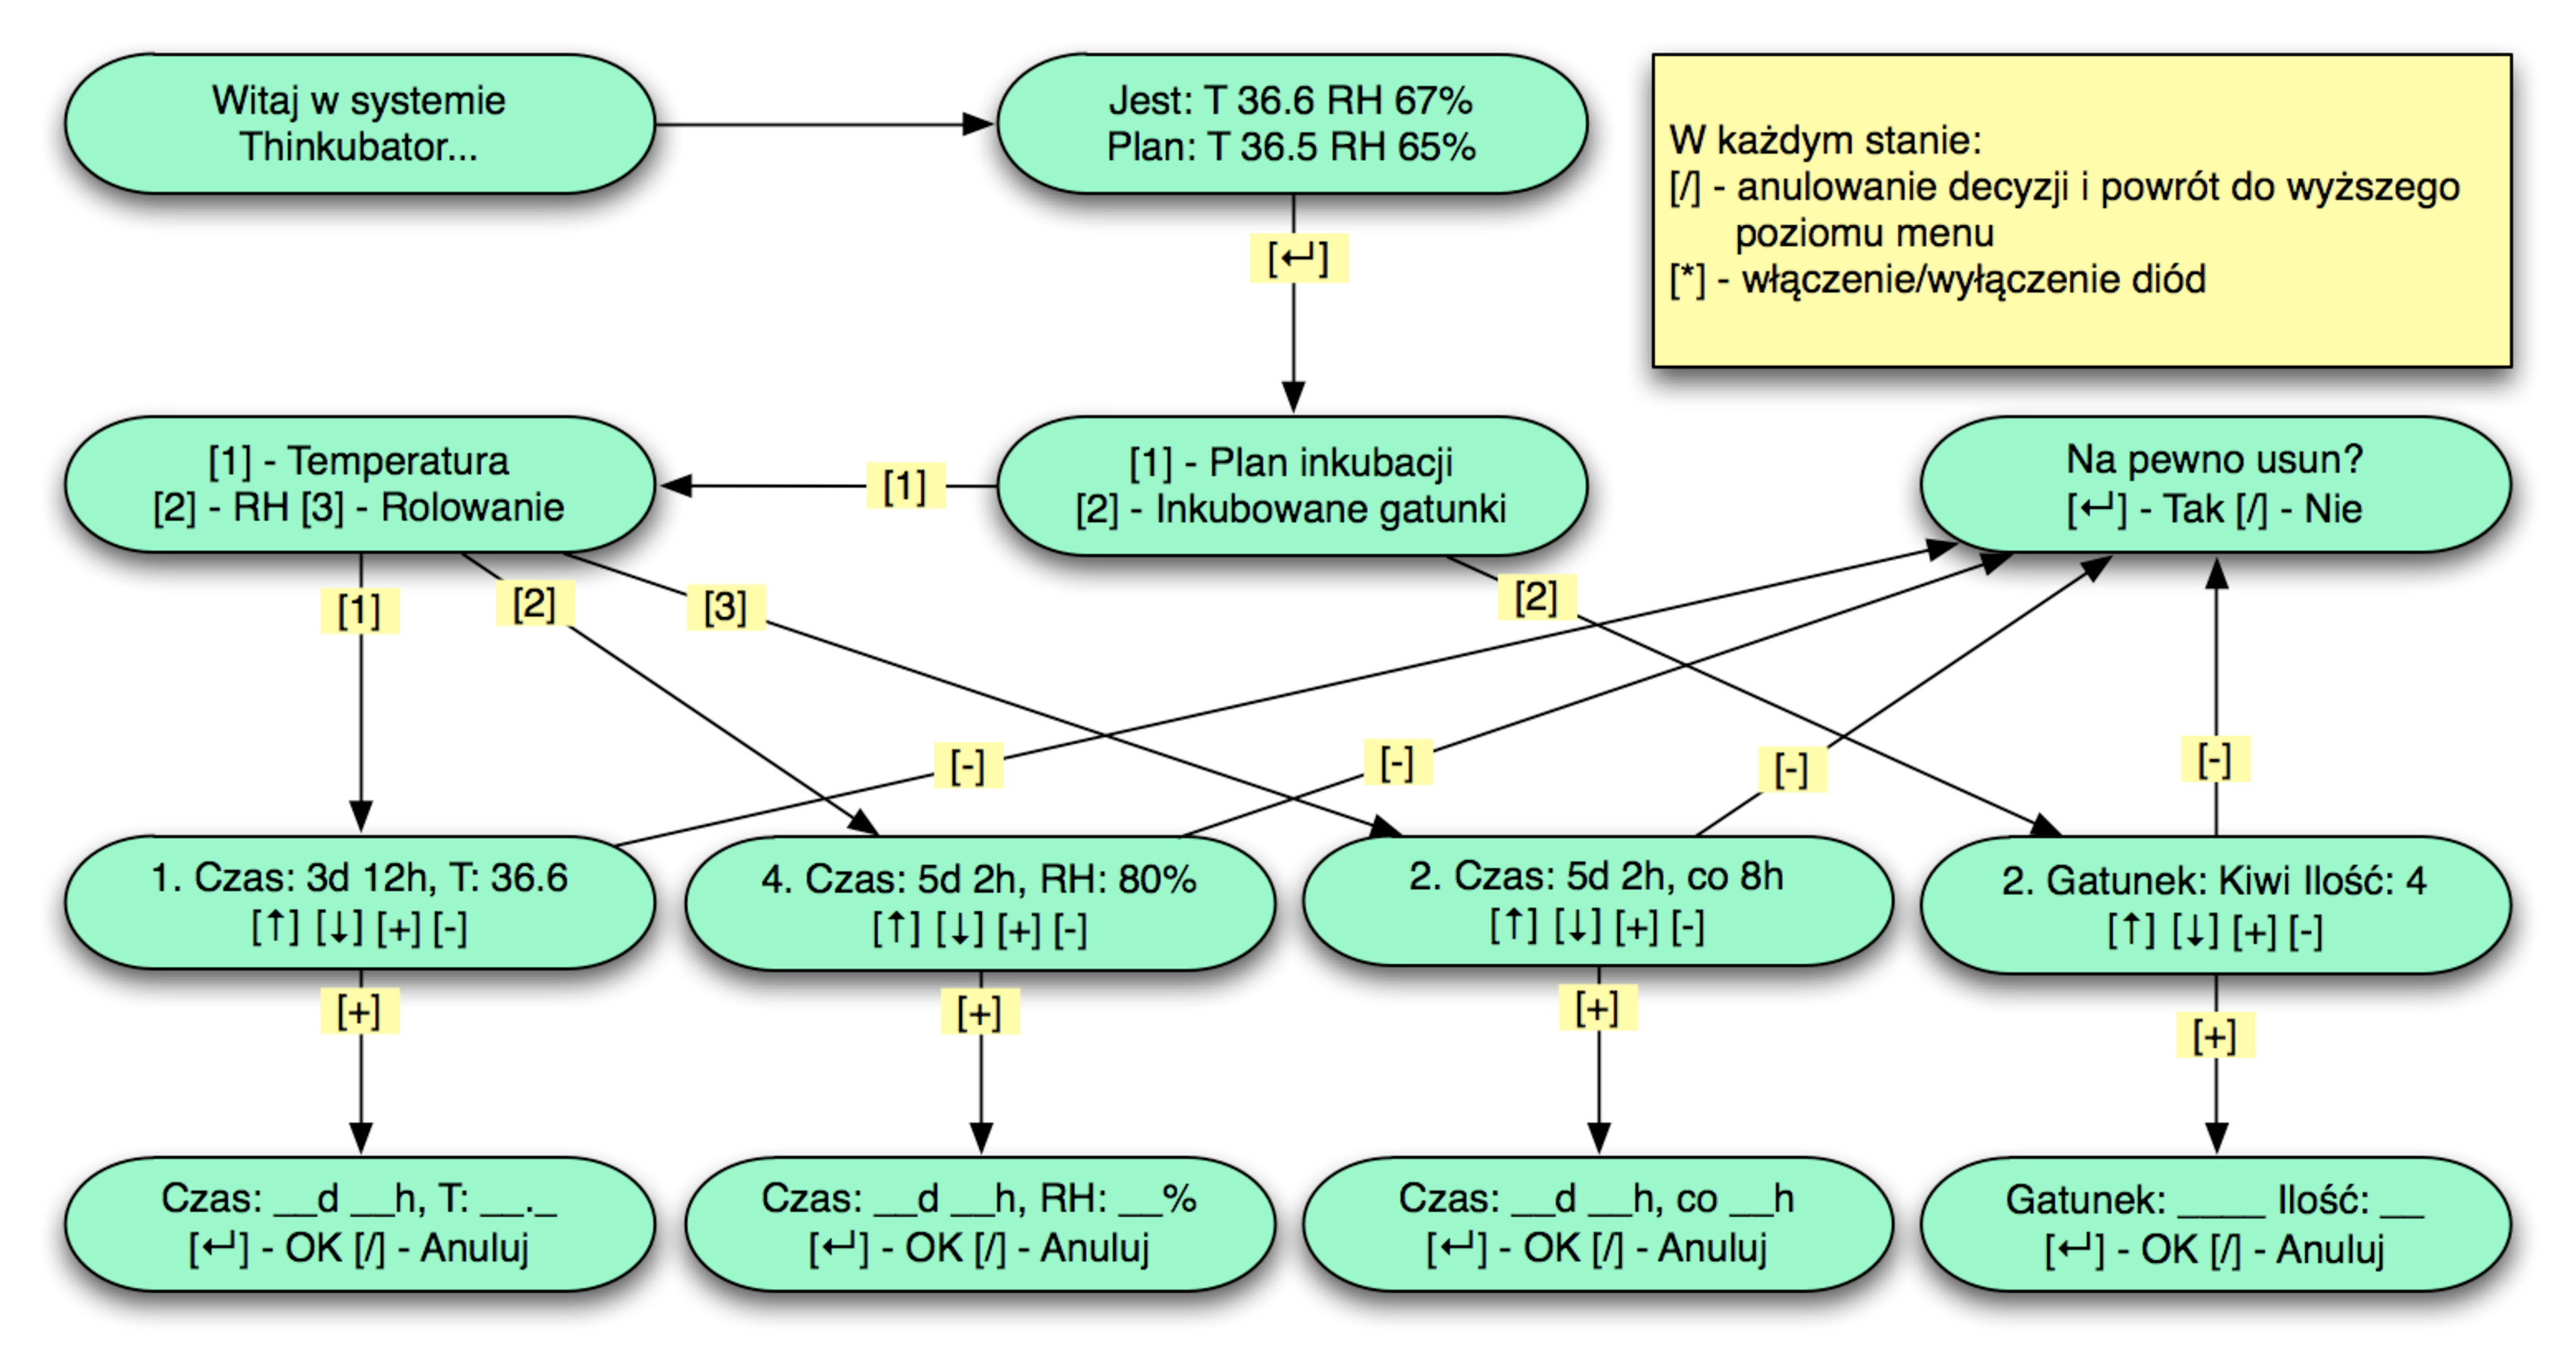
\includegraphics[width=\textwidth]{figures/Menu}
\caption{Diagram menu}\label{rys:Menu}
\end{figure}

\subsection{System operacyjny}
Aplikacja została zaimplementowana na system operacyjny Linux. Wybrano ten
system operacyjny gdyż potrzebowano pełnowymiarowego systemu operacyjnego, który
zapewniłby:
\begin{itemize}
 \item stos TCP/IP,
 \item kontrolę nad współbieżnością,
 \item biblioteki zapewniające dogodny dostęp do portów i~protokołów komunikacyjnych.
\end{itemize}
Wybór padł właśnie na system Linux, ponieważ dodatkowo:
\begin{itemize}
 \item ma silne środowisko do implementacji,
 \item zapewnia łatwość rekonfiguracji systemu -- dostosowanie systemu do posiadanej platformy sprzętowej,
 \item jest dobrze znany członkom zespołu.
\end{itemize}

\section{Komunikacja}
Ogólny przebieg komunikacji pomiędzy elementami systemu przedstawia
rysunek~\ref{rys:Komunikacja}. Linie czerwone oznaczają połączenia nawiązywane
za pomocą gniazd BSD, zielone -- XML-RPC, czarne -- HTTP.
\begin{figure}[b] 
\centering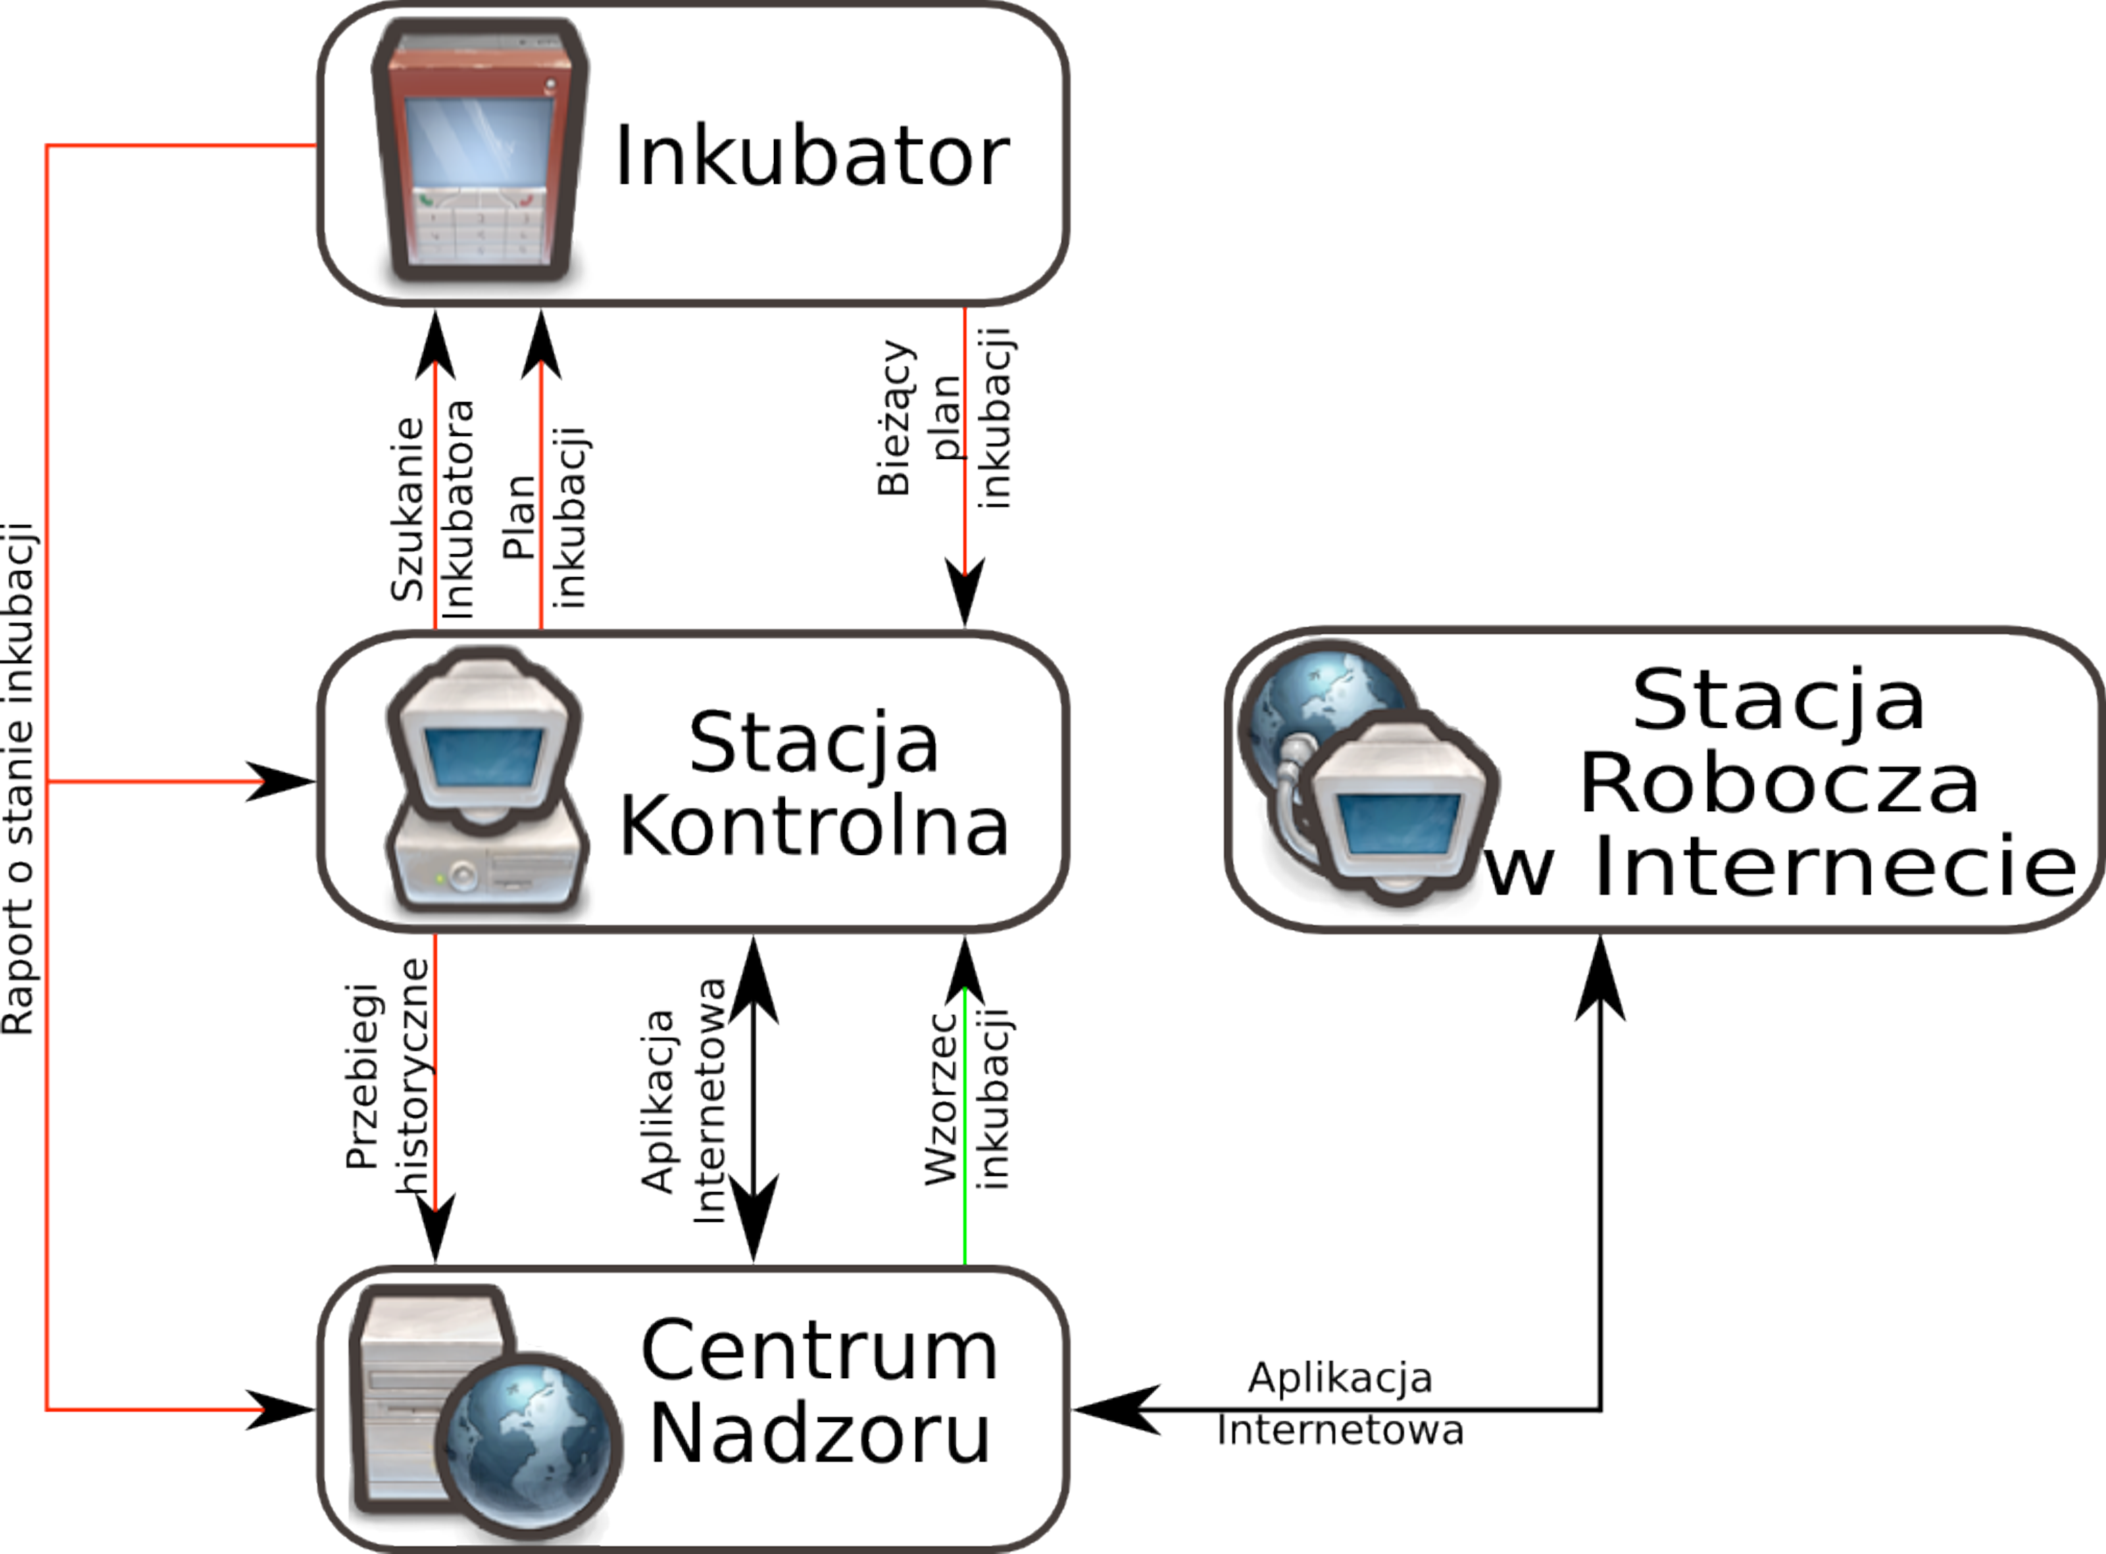
\includegraphics[width=.75\textwidth]{figures/Komunikacja}
\caption{Diagram komunikacji}\label{rys:Komunikacja}
\end{figure}

\subsection{Wykorzystane metody komunikacji}
\paragraph{Interfejs gniazd BSD}
System Thinkubator został zaimplementowany przy użyciu różnych języków
programowania (C, C\#, Phyton) oraz na różnych systemach operacyjnych (Gentoo
Linux, Windows XP), dlatego pożądany był sprawdzony interfejs komunikacji
sieciowej wspierany przez wszystkie powyższe technologie. Interfejs gniazd
został wykorzystany przy komunikacji na drodze Inkubator $\leftrightarrow$ Stacja Kontrolna,
Inkubator $\rightarrow$ Centrum Nadzoru oraz Stacja Kontrolna $\leftrightarrow$ Centrum Nadzoru.

W~każdej aplikacji uruchomiony jest osobny wątek odpowiedzialny za
odbieranie połączeń przychodzących. Wątek taki otwiera gniazdo na odpowiednim
porcie i~nasłuchuje na połączenia. W~momencie nawiązania połączenia wątek
nasłuchujący uruchamia kolejny wątek do obsługi połączenia, po czym powraca do
nasłuchiwania na nowe połączenia. Dzięki temu jakikolwiek błąd komunikacji nie
jest w~stanie zawiesić głównego wątku oczekującego na połączenia. Wykorzystane
porty to:
\begin{itemize}
	\item w~Inkubatorze port UDP BROADCAST\_PORT -- nasłuchiwanie na komunikat
		rozgłoszeniowy wysyłany przez Stację Kontrolną,
	\item w~Inkubatorze port TCP SCHEDULE\_PORT -- służący do odbierania ze Stacji
		Kontrolnej poleceń dotyczących pobrania/wysłania planu inkubacji, 
	\item w~Stacji Kontrolnej port TCP STATE\_REPORT\_PORT -- odbiór raportów
	z~inkubatora,
	\item w~Centrum Nadzoru port TCP STATE\_REPORT\_PORT -- odbiór raportów
	z~inkubatora lub Stacji Kontrolnej.
\end{itemize}

W~celu ujednolicenia protokołu komunikacji wszystkie pakiety przesyłane tą drogą
są zamknięte w~jedną z~dwóch struktur: struktura sterująca i~struktura danych.
Każdy akt komunikacji rozpoczyna się od przesłania jednej struktury sterującej
z~informacją o~typie rozkazu/komunikacji, który określa dalszy przebieg
komunikacji. Struktura danych służy do przesyłania raportów z~inkubatora,
historycznych przebiegów inkubacji oraz planów inkubacji. Definicja struktur
została przedstawiona w tabeli \ref{tab:Struktury}.
\begin{table}[t]
	\centering
	\begin{tabular}{m{7cm}|m{7cm}}
		\textbf{Control Structure:} &~\textbf{Data Structure:} \\
		& \verb+struct point_t {+ \\
		\verb+struct message_t {+ &~\verb+ int timestamp;+ \\
		\verb+ int deviceID;+ &~\verb+ int process_phase;+ \\
		\verb+ int processID;+ &~\verb+ double temperature;+ \\
		\verb+ int type;+ &~\verb+ double humidity;+ \\
		\verb+ int from_time;+ &~\verb+ int rolling;+ \\
		\verb+ int to_time;+ &~\verb+ double scheduled_temperature;+ \\
		\verb+ int amount;+ &~\verb+ double scheduled_humidity;+ \\
		\verb+}+ &~\verb+ int scheduled_rolling;+ \\
		& \verb+}+ \\
	\end{tabular}
	\caption{Definicja struktur komunikacyjnych}
	\label{tab:Struktury}
\end{table}

Ogólnie jednorazowa komunikacja odbywa się według algorytmu:
\begin{verbatim}
send( message_t header );
for i:=1 to header.amount do 
 send( point_t data );\end{verbatim}

\paragraph{Częściowe XML-RPC}
Stacja Kontrolna stosuje żądanie 
HTTP-GET do przesłania parametrów wywołania lub HTTP-POST do wysyłania danych
, zaś Centrum Nadzoru używa języka XML do
zakodowania wyników wywołania oraz HTTP jako protokołu transportowego. XML-RPC
jest również niezależny od platformy sprzętowej i~języka programowania. 
Odpowiedź XML dostosowana jest do formatu w~jakim Stacja Kontrolna przechowuje swoje dane. 
Technologia ta została wykorzystana gdy:
\begin{itemize}
\item Stacja Kontrolna pobiera z~Centrum Nadzoru wzorce inkubacji, 
\item Stacja Kontrolna pobiera z~Centrum Nadzoru informacje o~znanych gatunkach,
\item Stacja Kontrolna wysyła do Centrum Nadzoru informację o~rozpoczęciu inkubacji,
\item Stacja Kontrolna wysyła do Centrum Nadzoru informację o~zakończeniu inkubacji,
\end{itemize}

\section{Stacja kontrolna}
Aplikacja działająca na Stacji Kontrolnej została napisana w~środowisku
Visual Studio .NET 2005 \cite{MSDN}, w~języku programowania C\#. Ponadto program
wykorzystuje zewnętrzną bibliotekę graficzną \akronim{CSGL} (\english{C\#
Graphics Library}). Stacja Kontrolna spełnia dwa główne
zdania: monitorowanie oraz programowanie inkubatorów.

Monitorowanie realizowane jest poprzez mechanizm wysyłania z~inkubatorów
raportów z~wartościami sterowanych parametrów inkubacji. W~równych odstępach czasu Stacja Kontrolna rejestruje pakiet
danych od inkubatora z~informacją o~zaplanowanych i~aktualnych warunkach
panujących w~inkubatorze. Na tej podstawie Stacja Kontrolna wyświetla na ekranie aktualny stan
wszystkich zarejestrowanych inkubatorów oraz ogólny przebieg temperatury
i~wilgotności w~ciągu ostatniej doby. Po wybraniu dowolnego inkubatora Stacja Kontrolna
wyświetla szczegółowy przebieg sterowanych parametrów, obejmujący pełny okres
inkubacji. Dzięki wykorzystaniu biblioteki \emph{CSGL} możliwa jest płynna nawigacja
po wykresie, zbliżenie na dowolny okres czasu lub dowolne wartości temperatury
i~wilgotności.

Funkcjonalność programowania inkubatora pozwala na precyzyjny dobór nastawu inkubatora
w~bardzo prosty sposób. Przy tworzeniu nowego planu inkubacji ornitolog wybiera
inkubowane gatunki, zaś Stacja Kontrolna dobiera do nich wzorce inkubacji i~wizualizuje je na
ekranie. Półprzezroczyste wzorce inkubacji dla różnych gatunków są nakładane na siebie,
dzięki czemu widoczne są rozbieżności w~pożądanych przebiegach
temperatury i~wilgotności. Pozwala to na podjęcie decyzji o~dopuszczeniu różnych
gatunków do wspólnej inkubacji i~dobór optymalnego planu inkubacji. Utworzony
plan inkubacji może zostać zapisany na dysku lub przesłany do wybranego
inkubatora. Stacja Kontrolna pozwala też na pobranie z~inkubatora jego aktualnego planu
i~wprowadzenie w~nim dowolnych zmian.

\begin{figure}[b] 
\centering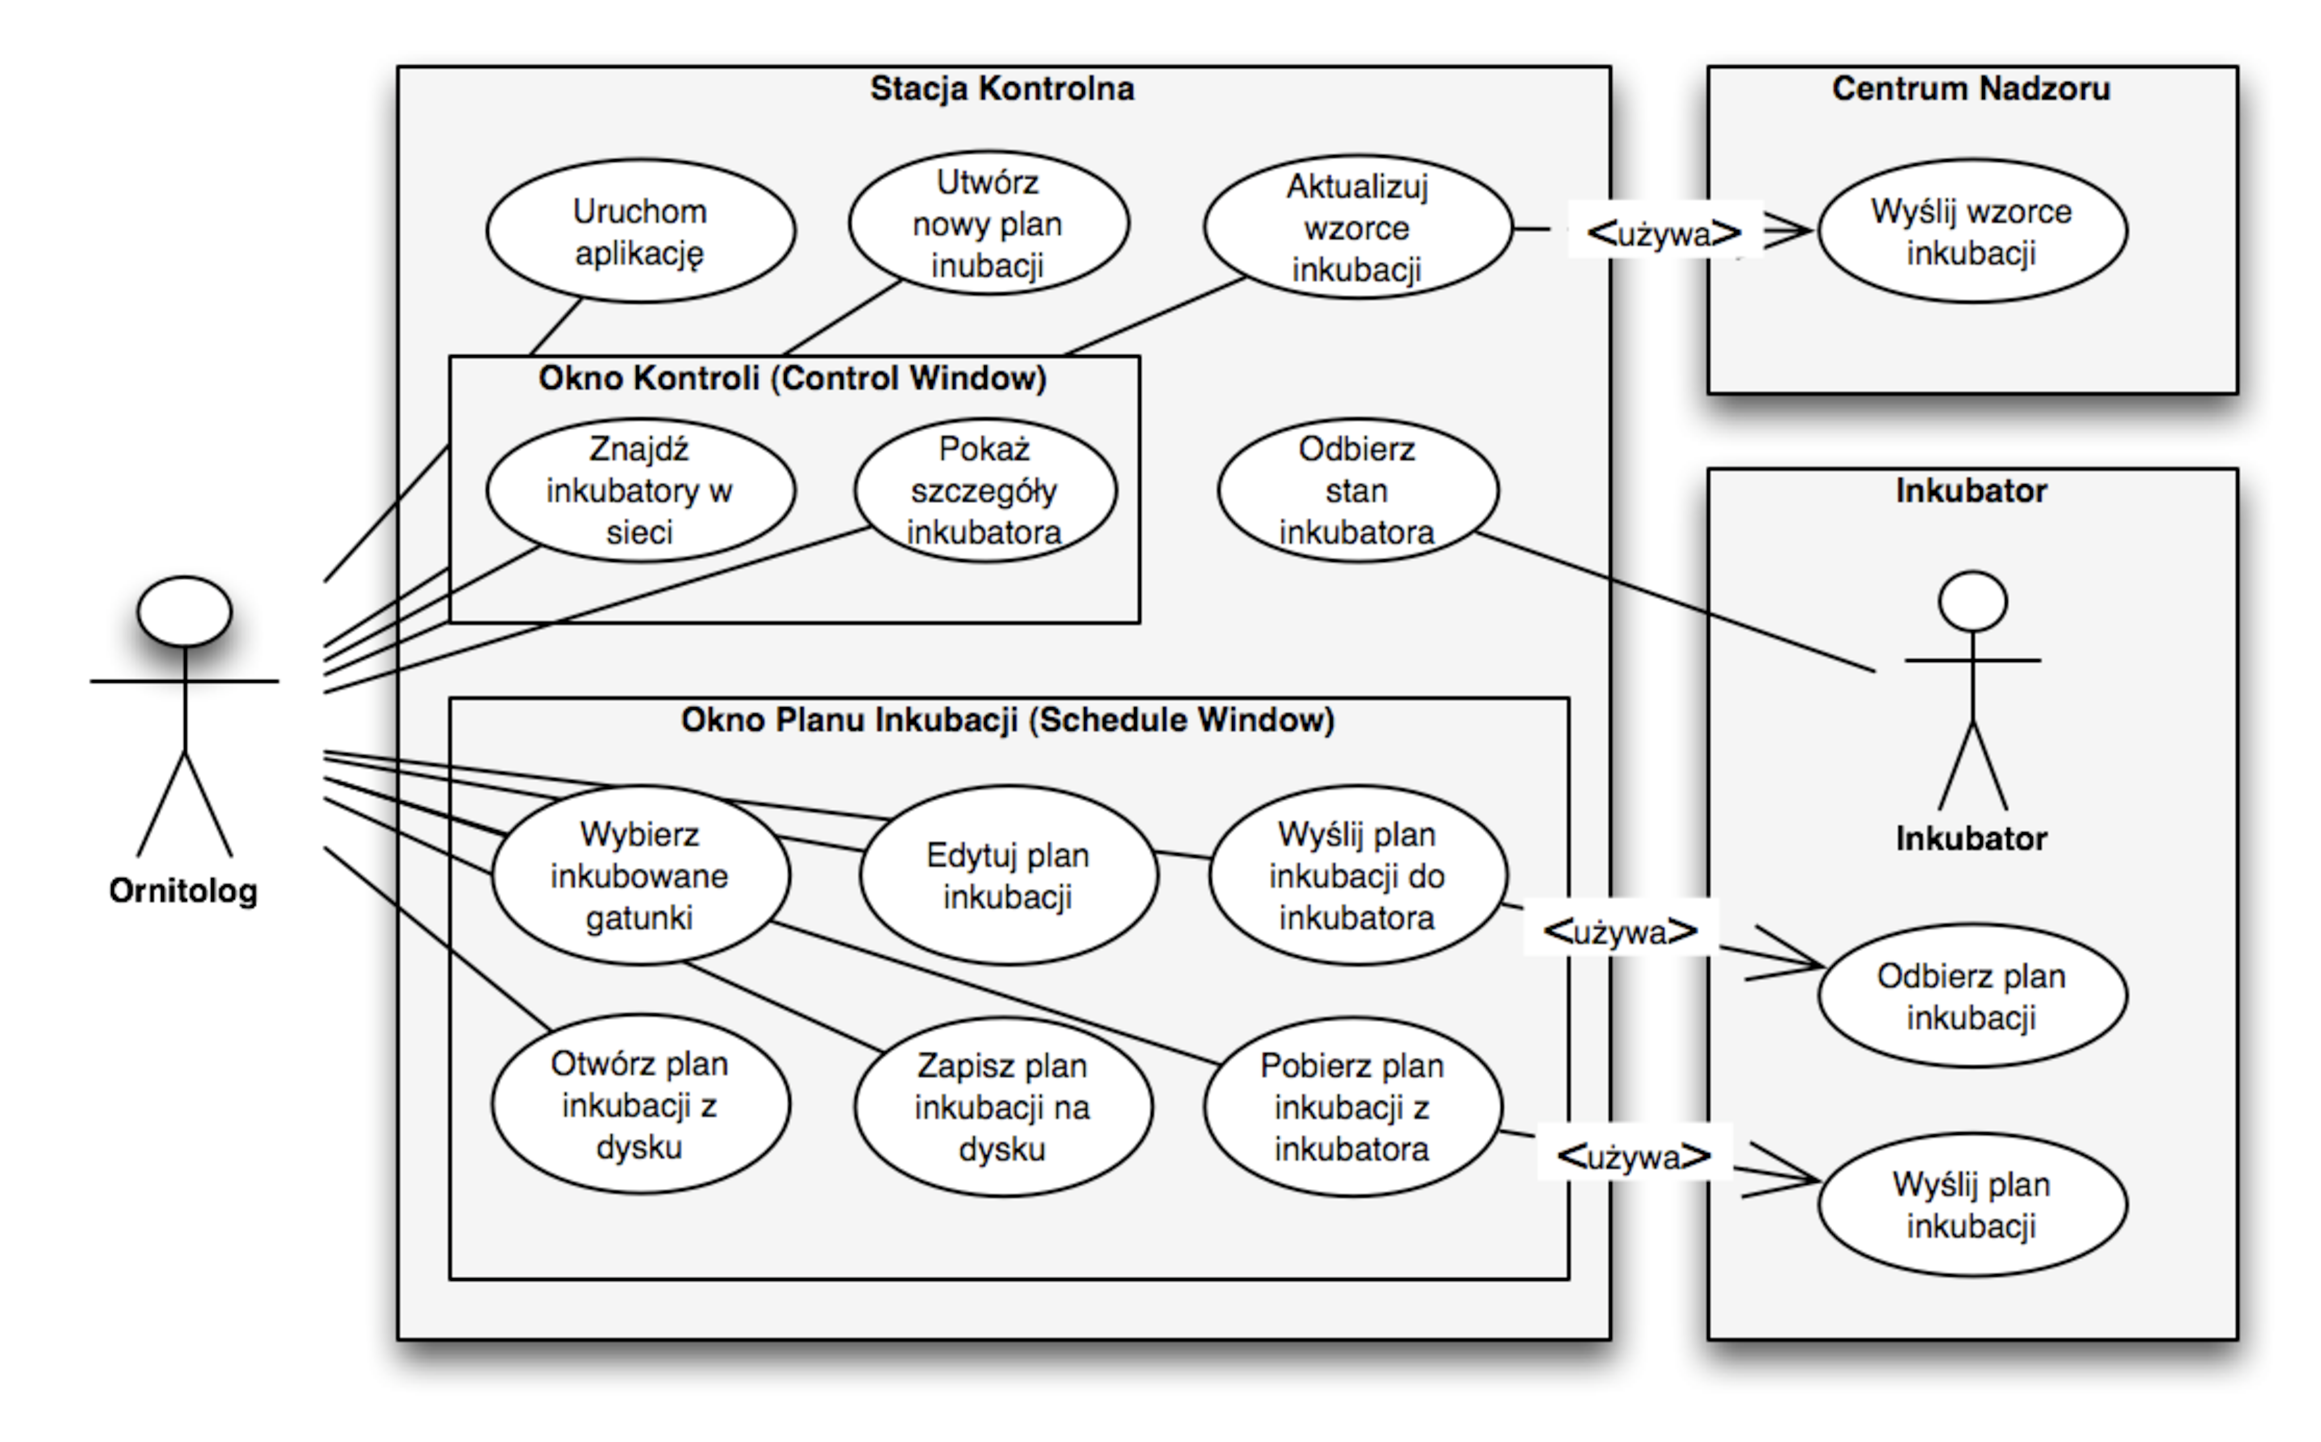
\includegraphics[width=\textwidth]{figures/CSUseCase}
\caption{Diagram przypadków użycia stacji kontrolnej}\label{rys:CSUseCase}
\end{figure}

\subsection{Przypadki użycia}
Podczas projektowania aplikacji przeprowadzono konsultacje z~użytkownikami końcowymi
i~przeanalizowano wymaganą oraz pożądaną funkcjonalność programu.
W rezultacie wyznaczono 12 przypadków użycia, które ilustruje rysunek \ref{rys:CSUseCase}. 
\pagebreak

\noindent Poszczególne przypadki użycia zdefiniowane są następująco:\\
Aktorzy:
\begin{enumerate}
	\item Ornitolog -- osoba przeprowadzająca/nadzorująca inkubację,
	\item Inkubator -- aplikacja inkubatora,
	\item Stacja Kontrolna -- opisywany system,
	\item Centrum Nadzoru -- zdalny serwer.
\end{enumerate}

\begin{itemize}
	\item[\textbf{UC1}] Uruchomienie aplikacji.
		\begin{enumerate}
			\item Ornitolog uruchamia aplikację Stacji Kontrolnej.
			\item Stacja Kontrolna uruchamia wątek oczekujący na przychodzące połączenia z~sieci.
			\item Stacja Kontrolna wysyła w~sieć lokalną wiadomość rozgłoszeniową z~własnym adresem IP, celem poinformowania o~nim Inkubatorów.
			\item Stacja Kontrolna oczekuje klika sekund na odpowiedź Inkubatorów.
			\item Stacja Kontrolna rejestruje znalezione Inkubatory.
			\item Stacja Kontrolna wyświetla główne okno aplikacji, Control Window.
		\end{enumerate}

	\item[\textbf{UC2}] Znajdź inkubatory w~sieci.
		\begin{enumerate}
			\item Ornitolog wybiera z~menu opcję ,,Find incubators''.
			\item Stacja Kontrolna wysyła w~sieć lokalną wiadomość rozgłoszeniową z~własnym adresem IP, celem poinformowania o~nim Inkubatorów.
			\item Stacja Kontrolna oczekuje klika sekund na odpowiedź Inkubatorów.
			\item Stacja Kontrolna rejestruje znalezione Inkubatory.
		\end{enumerate}


	\item[\textbf{UC3}] Pokaż szczegóły inkubatora.
		\begin{enumerate}
			\item Ornitolog wybiera jeden z~inkubatorów widocznych w~głównym oknie aplikacji.
			\item Stacja Kontrolna wyświetla szczegółowy wykres wybranego inkubatora.
			\item Ornitolog dowolnie nawiguje po wykresie, manipulując osiami czasu, temperatury i~wilgotności.
		\end{enumerate}

	\item[\textbf{UC4}] Utwórz nowy plan inkubacji.
		\begin{enumerate}
			\item Ornitolog wybiera opcję ,,Schedule Tool'' z~menu aplikacji.
			\item Stacja Kontrolna wyświetla okno do tworzenia planu inkubacji (Schedule Window).
		\end{enumerate}

	\item[\textbf{UC5}] Edytuj listę gatunków.
		\begin{enumerate}
			\item Ornitolog wybiera z~menu opcję ,,Birds''.
			\item Stacja Kontrolna wyświetla dialog wyboru gatunków.
			\item Ornitolog wybiera inkubowane gatunki i~zatwierdza wybór.
			\item Stacja Kontrolna aktualizuje wzorzec inkubacji w~oknie planu inkubacji.
		\end{enumerate}

	\item[\textbf{UC6}] Zapisz plan inkubacji na dysku.
		\begin{enumerate}
			\item Ornitolog wybiera z~menu opcję zapisania planu inkubacji (,,Save'').
			\item Stacja Kontrolna wyświetla dialog wyboru pliku.
			\item Ornitolog wybiera plik do zapisu planu inkubacji.
			\item Stacja Kontrolna zapisuje plan inkubacji.
		\end{enumerate}

	\item[\textbf{UC7}] Wczytaj plan inkubacji z~dysku.
		\begin{enumerate}
			\item Ornitolog wybiera z~menu opcję wczytania planu inkubacji (,,Open'').
			\item Stacja Kontrolna wyświetla dialog wyboru pliku.
			\item Ornitolog wybiera plik do wczytania planu inkubacji.
			\item Stacja Kontrolna wczytuje plan inkubacji.
		\end{enumerate}

	\item[\textbf{UC8}] Edytuj plan inkubacji.
		\begin{enumerate}
			\item Ornitolog wybiera z~paska narzędzi edytowaną funkcję (temperatura, wilgotność lub rolowanie).
			\item Ornitolog nanosi wartości pożądanej funkcji na wykres.
		\end{enumerate}

	\item[\textbf{UC9}] Wyślij plan inkubacji do inkubatora.
		\begin{enumerate}
			\item Ornitolog wybiera z~menu opcję wysłania planu inkubacji do Inkubatora (,,Send schedule'').
			\item Stacja Kontrolna wyświetla dialog wyboru inkubatora.
			\item Ornitolog wybiera inkubator.
			\item Stacja Kontrolna wysyła do Inkubatora informację o~zmianie planu inkubacji.
			\item Inkubator akceptuje zmianę.
			\item Stacja Kontrolna wysyła plan inkubacji.
			\item Inkubator odbiera plan inkubacji.
			\item Stacja Kontrolna informuje Ornitologa o~poprawnie wykonanej operacji.
		\end{enumerate}

	\item[\textbf{UC10}] Pobierz plan inkubacji z~inkubatora.
		\begin{enumerate}
			\item Ornitolog wybiera z~menu opcję pobrania planu inkubacji do inkubatora (,,Retrieve schedule'').
			\item Stacja Kontrolna wyświetla dialog wyboru inkubatora.
			\item Ornitolog wybiera inkubator.
			\item Stacja Kontrolna wysyła do Inkubatora żądanie planu inkubacji.
			\item Inkubator wysyła plan inkubacji.
			\item Stacja Kontrolna odbiera plan inkubacji.
			\item Stacja Kontrolna wyświetla pobrany plan inkubacji.
			\item Stacja Kontrolna informuje Ornitologa o~poprawnie wykonanej operacji.
		\end{enumerate}

	\item[\textbf{UC11}] Aktualizuj wzorce inkubacji.
		\begin{enumerate}
			\item Ornitolog wybiera z~menu opcję uaktualnienia wzorców.
			\item Stacja Kontrolna pobiera wzorce inkubacji z~Centrum Nadzoru poprzez HTTP.
			\item Stacja Kontrolna informuje Ornitologa o~poprawnie wykonanej operacji.
		\end{enumerate}

	\item[\textbf{UC12}] Odbierz stan inkubatora.
		\begin{enumerate}
			\item Inkubator wysyła do Stacji Kontrolnej pakiet danych pomiarowych z~informacją o~warunkach panujących aktualnie w~komorze inkubacyjnej.
			\item Stacja Kontrolna odbiera pakiet danych.
			\item Jeśli inkubator nie był wcześniej wykryty, zostaje on zarejestrowany w~Stacji Kontrolnej.
			\item Stacja Kontrolna dodaje otrzymany pakiet danych do historii inkubacji danego Inkubatora.
			\item Stacja Kontrolna zapisuje historię inkubacji danego Inkubatora na dysku.
		\end{enumerate}
\end{itemize}


\subsection{Architektura aplikacji}
Architektura aplikacji Stacji Kontrolnej zgodna jest z~podziałem funkcjonalności na monitorowanie i~programowanie inkubatorów.
Funkcje te zostały zaimplementowane w~dwóch klasach dziedziczących
z~klasy \emph{Form}, o~nazwie odpowiednio \emph{ControlWindow} i~\emph{ScheduleWindow}. Okna te są zintegrowane
w~głównym oknie aplikacji (\emph{ControlStation}). Algorytmy komunikacji sieciowej implementuje statyczna klasa
\emph{Listener}. Klasa ta zawiera również kolekcję obiektów klasy \emph{Icubator}, które reprezentują znajdujące się w~sieci Inkubatory.
Szczegółowy diagram klas przedstawiony jest na rysunku~\ref{rys:CSClass}.

\begin{figure}[h] 
\centering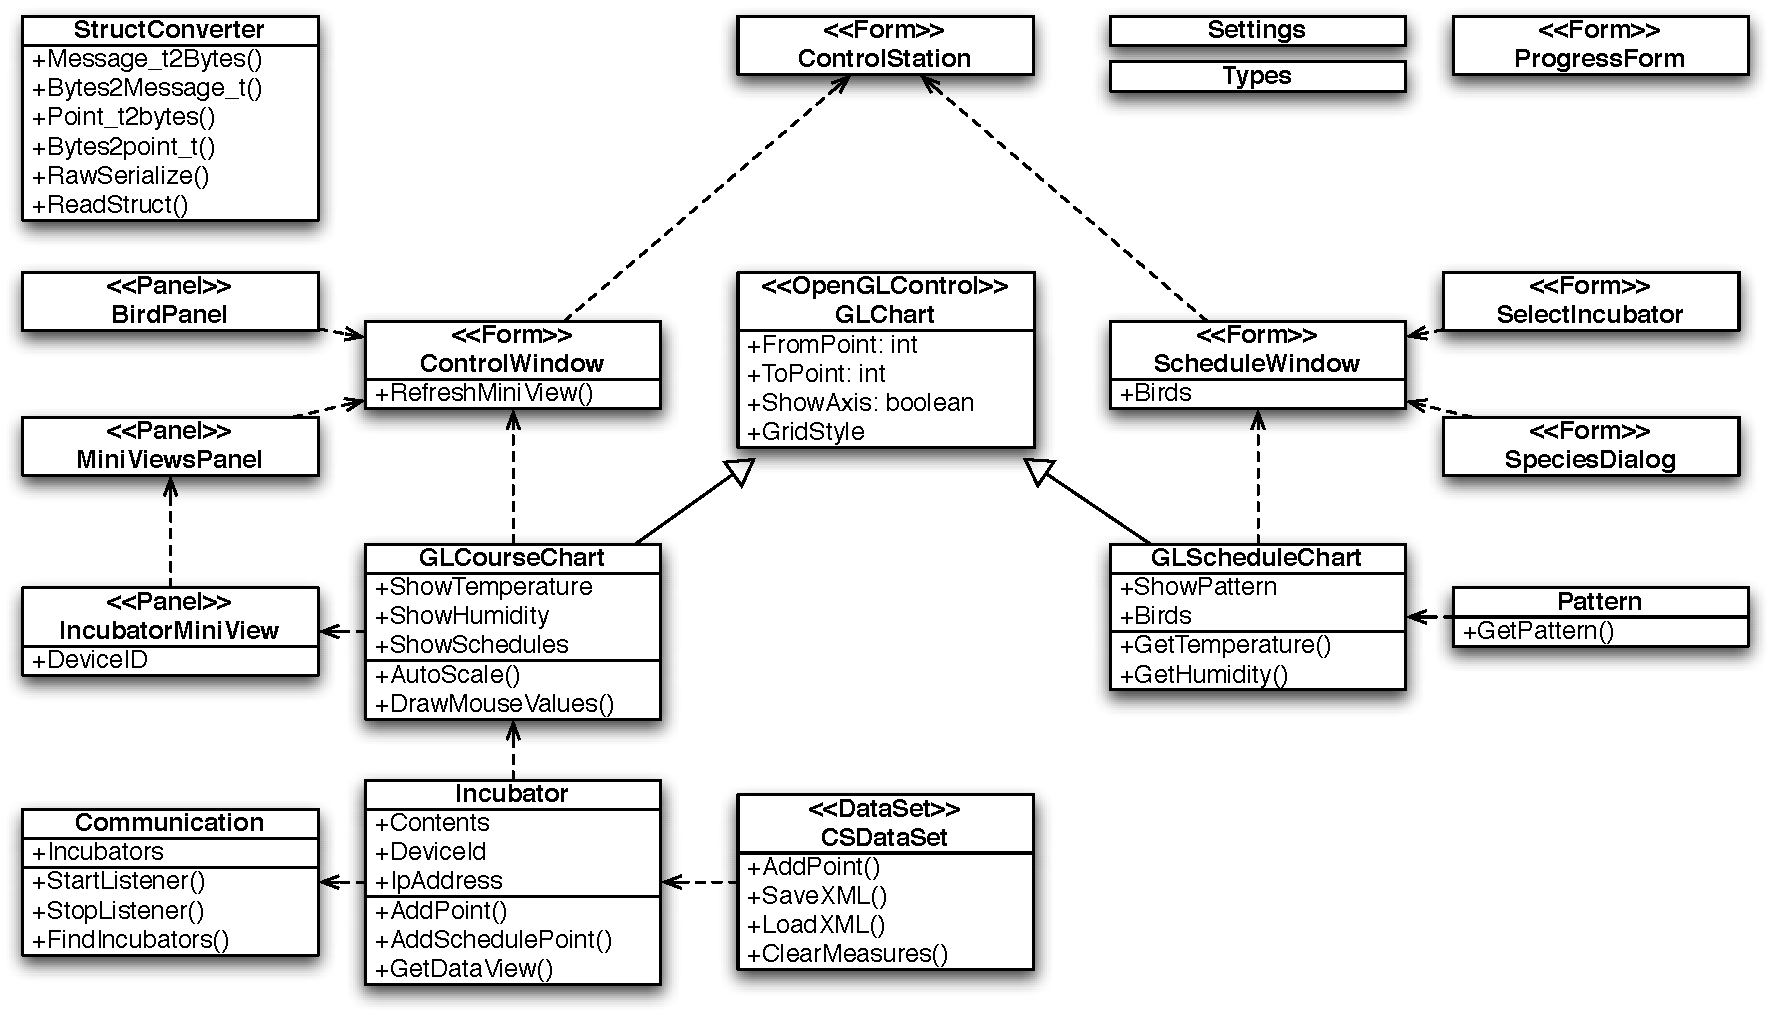
\includegraphics[width=\textwidth]{figures/CSClass}
\caption{Diagram klas aplikacji działającej na Stacji Kontrolnej}\label{rys:CSClass}
\end{figure}

\noindent Opis klas tworzących aplikację Stacji Kontrolnej:
\begin{itemize}
	\item ControlStation -- główne okno aplikacji,
	\item ControlWindow -- okno kontrolne, zawsze otwarte w~głównym oknie aplikacji, zawiera widok listy inkubatorów i~podgląd wybranego inkubatora,
	\item GLChart -- kontrolka dziedzicząca z~klasy \emph{OpenGLControl} umożliwiająca renderowanie wykresów przy użyciu biblioteki \emph{CSGL},
	\item GLCourseChart -- kontrolka dziedzicząca z~klasy \emph{GLChart}, dostosowana do renderowania przebiegów temperatury i~wilgotności,
	\item MiniViewsPanel -- kontrolka, na której wyświetlana jest lista kontrolek typu \emph{IncubatorMiniView},
	\item IncubatorMiniView -- kontrolka, na której wyświetlana jest informacja o~warunkach panujących w~inkubatorze oraz wykres temperatury i~wilgotności z~ostatniej doby,
	\item BirdPanel -- kontrolka, na której wyświetlana jest lista gatunków w~wybranym inkubatorze,
	\item ScheduleWindow -- okno do programowania inkubatora,
	\item ScheduleChart -- kontrolka dziedzicząca z~klasy \emph{GLChart}, dostosowana do nanoszenia planu inkubacji,
	\item Pattern -- klasa reprezentująca wzorce inkubacji,
	\item SpeciesDialog -- dialog wyboru inkubowanych gatunków,
	\item SelectIncubator -- dialog wyboru inkubatora, służy do wysyłania i~pobieranie planu inkubacji z~inkubatora,
	\item Incubator -- klasa reprezentująca inkubator, zawiera informacje o~zawartości inkubatora i~bieżącym procesie inkubacji,
	\item CSDataSet -- zbiór danych pomiarowych z~przebiegu inkubacji,
	\item Communication -- statyczna klasa odpowiedzialna za komunikację sieciową, zawiera inkubatory zarejestrowane w~systemie,
	\item ProgressForm -- okno z~paskiem postępu wyświetlanym w~trakcie szukania inkubatorów,
	\item Settings -- ustawienia aplikacji zapamiętywane w~rejestrze systemowym,
	\item Types -- klasa zawierająca definicję typów strukturalnych i~wyliczeniowych,
	\item TimeConverter -- statyczna klasa udostępniająca metody konwersji czasu między
		formatami stosowanymi w~C\# i~C,
	\item StructConverter -- statyczna klasa udostępniająca metody konwersji struktur do strumienia bajtów wysyłanych przez sieć.
\end{itemize}

\section{Centrum nadzoru}
%[[Tak jak można by powiedzieć że inkubatory to mięśnie naszego systemu, a~stacje kontroli -- nerwy, to serwer jest mózgiem naszego systemu.]]
Centrum Nadzoru jest dopełnieniem systemu Thinkubator, które choć nie jest niezbędne
do prowadzenia inkubacji, to daje niespotykane dotychczas możliwości. Jest ono odpowiedzialne za:
\begin{itemize}
	\item gromadzenie danych z~przebiegu inkubacji (zaprogramowane i~rzeczywiste wartości sterowanych parametrów),
	\item monitorowanie bieżącego stanu inkubatorów,
	\item wizualizacja dotychczasowego przebiegu każdej inkubacji,
	\item informowanie o~stanie wiedzy na temat gatunków,
	\item analiza danych celem tworzenia wzorców,
	\item alarmowanie o~błędach,
	\item kontrola dostępu użytkowników do poszczególnych funkcji systemu,
	\item zarządzanie kontami użytkowników.
\end{itemize}
W tej chwili nie ma ono pełnej oczekiwanej funkcjonalności gdyż analiza danych w~takim systemie to bardzo złożony problem wymagający długotrwałych badań zarówno na poziomie informatyki jak i~biologii. Obecna implementacja jest podstawą do dalszego rozwoju.

\subsection{Technologia}
Ze względu na krótki czas rozwoju i~duże wymagania dla Centrum Nadzoru, do
implementacji postanowiono użyć środowiska progamistycznego TurboGears
\cite{TurboGears} napisanego w~języku Python. Jest to jedno z~najnowszych
z~narzędzi służących do rozwoju internetowych aplikacji w~architekturze
\akronim{MVC} (\english{Model, View, Controller}). Wnioski z~testów
przeprowadzonych przez niezależnego eksperta sugerują, że można około 9~razy
szybciej rozwijać aplikacje internetowe w~TG niż przy użyciu \akronim{J2EE}
(\english{Java 2~Enterprise Edition}), zakładając że wykorzystano
\emph{Hibernate} jako warstwę trwałości. Przy zastosowaniu \akronim{EJB}
(\english{Enterprise JavaBeans}) przewaga TG rośnie jeszcze bardziej, oczywiście
w~teście założono nierozróżnialność jakościową (funkcjonalność, wydajność itd.)
aplikacji. Oprócz tego TG udostępnia aplikacje do zarządzania bazą danych oraz
wspiera wykorzystanie \akronim{AJAX} (\english{Asynchronous JavaScript And
XML}), co będzie miało znaczenie również przy rozbudowywaniu naszego systemu.
TG aktywnie korzysta z~infrastruktury setuptools \cite{setuptools} -- dzięki
czemu można korzystać z~różnego rodzaju modułów przygotowanych i~udostępnianych
przez użytkowników systemu np.: generator wykresów PlotKit \cite{PlotKit}. Przy
tworzeniu bazy danych skorzystano z mapera obiektowo relacyjnego
\emph{SQLObject}. Jako bazę danych wykorzystano MySQL ze względu na jego
szybkość, łatwość obsługi i~dostępność dokumentacji. Warstwa trwałości jest
niezależna od bazy danych więc w~razie potrzeby można bazę danych zmienić. 

\subsection{Baza danych}
\begin{figure}[t]
\centering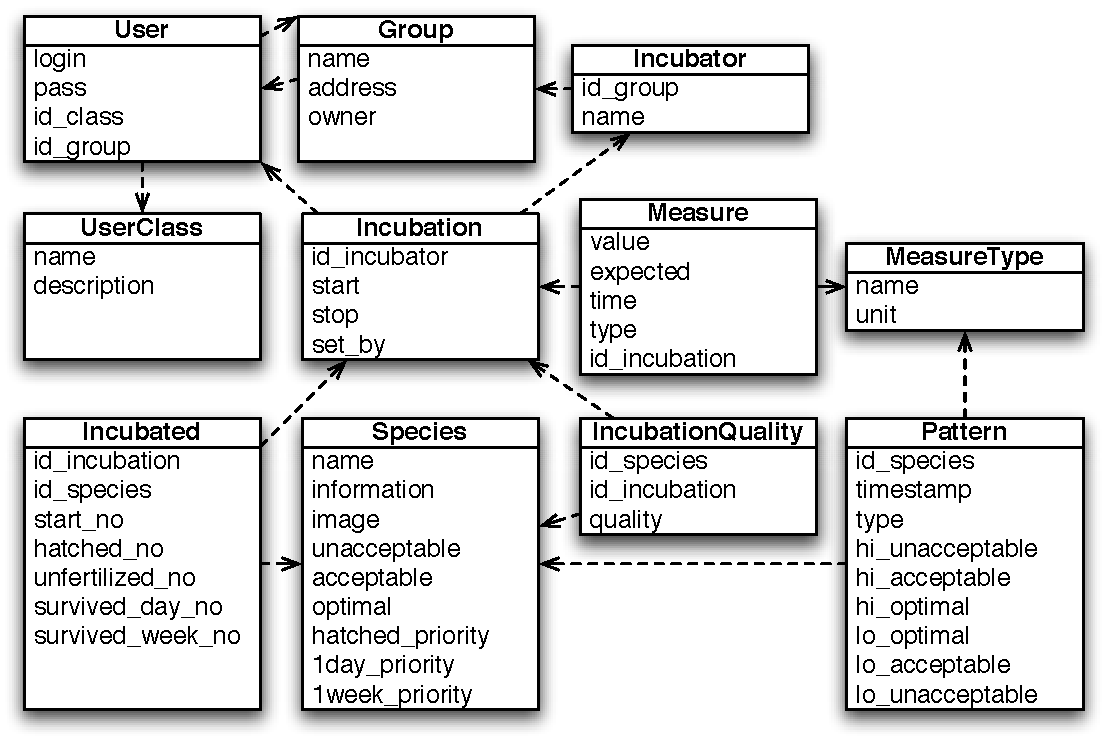
\includegraphics[width=\textwidth]{figures/SCCDataBase}
\caption{Schemat bazy danych centrum nadzoru}\label{rys:SCCDataBase}
\end{figure}

Relacyjny schemat tabel bazy danych przedstawiono na rysunku
\ref{rys:SCCDataBase}. Poniżej przedstawiony jest krótki opis tabel znajdujących
się na nim:
\begin{itemize}
	\item \textbf{Group} -- opisuje grupy użytkowników. Najczęściej
		występującą grupą będą pracownicy jakiejś instytucji mający dostęp do
		określonej puli Inkubatorów. Grupa ma właściciela (pole owner), może on
		edytować użytkowników grupy. 
	\item \textbf{User} -- opisuje Użytkowników systemu. Użytkownik może
		należeć do różnych klas z~tabeli UserClass.
	\item \textbf{UserClass} -- krotki w~tej tabeli odpowiadają klasom użytkowników.
		Dla każdej klasy użytkowników zdefiniowane są w~systemie pewne prawa
		dostępu. 
	\item \textbf{Incubator} -- opisuje Inkubatory. Inkubator należy do
		grupy użytkowników. Użytkownik może go opisać, aby było mu łatwo rozróżnić
		Inkubatory.
	\item \textbf{Measure} -- opisuje pomiary z~czujników w~Inkubatorze.
		Pomiar dotyczy inkubacji oraz ma typ z~tabeli MeasureType. Każdy pomiar jest
		również umiejscowiony w~czasie.
	\item \textbf{MeasureType} -- zawiera typy pomiarów (np. temperatura,
		wilgotność).
	\item \textbf{Incubation} -- opisuje inkubację: na którym inkubatorze
		jest przeprowadzona, w~jakim czasie i~kto ją zainicjował. 
	\item \textbf{Inlubated} -- opisuje wynik inkubacji dla danego gatunku.
		System zapamiętuje ilość jaj, ilość wyklutych piskląt oraz ilość
		piskląt, które przeżyły 24 godziny oraz pierwszy tydzień. Dla zoologów są to
		bardzo ważne dane gdyż większość piskląt umiera podczas pierwszego tygodnia po wykluciu.
		Może się więc okazać, że mimo iż pewne inkubacje są nierozróżnialne pod
		względem klujności, to przeżywalność w~dłuższym czasie się zmienia. 
	\item \textbf{Species} -- zawiera podstawowe dane o~gatunkach.
	\item \textbf{DataAnalisys} -- zawiera dane o~jakości inkubacji (pole
		,,parameters''). Są one generowane w~oparciu o~wartości pomiarów dla danej
		inkubacji oraz jej wynik. Jakość inkubacji jest wagą w~oparciu o~którą
		generowany jest wzorzec inkubacji dla danego gatunku. 
	\item \textbf{Pattern} -- przechowuje wzorzec inkubacji dla
		danego gatunku. Opisuje on chwile w~czasie i~przyporządkowuje im nastawy
		które są pożądane, dopuszczalne i~niedopuszczalne. Pole ,,type'' determinuje czy
		krotka opisuje wilgotność czy temperaturę. 
\end{itemize}

\subsection{Implementacja}
W~tym podrozdziale zostały opisane szczegóły implementacj Centrum Nadzoru.
Wynikają one z architektury TurboGears. Cała aplikacja składa się z~obiektów
czterech rodzajów:
\begin{itemize}
	\item \textbf{Wzorców} -- są to klasy wygenerowane z~języka wzorców Kid
		\cite{KID}. Wzorce reprezentują warstwę prezentacji aplikacji. Język Kid
		opiera się o~XHTML. Przy jego pomocy projektowane były komponenty Wizualne.
		Przed uruchomieniem aplikacji kontroler TurboGears zamienia wzorce na
		obiekty, które są wywoływane przez Kontrolery. 
	\item \textbf{Komponentów} -- są to klasy specyficzne dla TurboGears.
		Komponenty są klasami, które dodają do Wzorców pewną funkcjonalność. Wzorzec
		tylko wygląda, a~komponent jeszcze posiada pewną funkcjonalność. Komponent
		może się składać z~wielu innych komponentów (np. formularz) oraz z~wielu
		wzorców. Komponenty korzystają transparentnie z~biblioteki MochiKit,
		ułatwiając implementację komponentów korzystających z~technologii
		\akronim{AJAX}.
	\item \textbf{Klasy modelu} -- implementują one klasy mapera obiektowo
		relacyjnego \emph{SQLObject}. Klasy modelu reprezentują krotki w~bazie
		danych. Klasy modelu są typów zgodnych z~typami tabel bazy danych. Baza
		danych została utworzona w~oparciu implementację klas modelu.
	\item \textbf{Kontrolerów} -- implementują one elementy serwera Cherrypy.
		Kontrolery łączą ze sobą wszystkie pozostałe klasy. One wykonują zapytania
		w~oparciu o~dane wejściowe przy pomocy klas modelu,obrabiają je i~wywołują
		wzorce lub komponenty z~odpowiednimi parametrami.
\end{itemize}
W następnej części dokumnetu bardziej szczegółowo opisano najważniejsze części
aplikacji.

\paragraph{Kontrolery:}
\begin{itemize}
\item \textbf{Index} -- domyślny kontrtoler odpowiada za wygląd i~strukturę
	dokumentu.
\item \textbf{Info} -- jest on implementacją prostego systemu zarządzania
	treścią CMS, zawiera ogólne informacje o~projekcie.
\item \textbf{Incubators} -- implementuje system pozwalający śledzić stan
	inkubatorów,
\item \textbf{Incubations} -- ten kontroler pozwala śledzić stan inkubacji
	(zmienne procesowe inkubatora). Pozwala edytować ilość jaj poszczególnych
	gatunków oraz wyniki inkubacji. 
\item \textbf{Species} -- ten kontroler jest odpowiedzialny za wyświetlanie
	stanu wiedzy systemu o~poszczególnych gatunkach (np. ilość inkubacji, średnia
	klujność oraz wzorce inkubacji).
\item \textbf{Plotter} -- ten kontroler jest odpowiedzialny za generowanie
	odpowiednich wykresów.
\item \textbf{XML-RPC} zajmuje się odpowiadaniem na zapytania Stacji Kontrolnej.
	W momencie gdy Stacja kontrolna potwierdzi zakończenie inkubacji, uruchamia on
	także generator wzorców.
\item \textbf{Catwalk} jest komponentem służącym bezpośrednio do przeglądania bazy danych. W~tej chwili funkcjonalność administracyjna jest bardzo ograniczona. Zakłada się, że jest jeden administrator, który bezpośrednio edytuje zawartość bazy danych przy pomocy tego komponentu.
\end{itemize}

\paragraph{Generowanie wzorców.}
W tej chwili do dyspozycji jest prosty algorytm generujący wzorce, oparty
o~linearyzację wag inkubacji i~ich pomiarów. Dla każdej inkubacji liczona jest
jej waga ($W$), równoważna klujności danego gatunku w~danej inkubacji. Jest ona
liczona w~oparciu o~stosunek ilości piskląt, które się wykluły ($p_w$), piskląt,
które przeżyły 24 godziny ($p_{24}$) oraz piskląt, które przeżyły tydzień
($p_t$) oraz wag dla tych ilości ustalonych dla danego gatunku -- odpowiednio:
$w_w$, $w_{24}$ i~$w_t$, do ilości zalężonych jaj ($j_z$) pomnożonych przez sumę
wag. Końcowy wzór przedstawiono w równaniu \ref{eq:wagi}.

\begin{equation}
	\label{eq:wagi}
	W =~\frac{p_w \cdot w_w +~p_{24} \cdot w_{24} +~p_t \cdot w_t }{(w_w +~w_{24} +~w_t) \cdot j_z} 
\end{equation}

W każdym punkcie pomiarowym generowana jest funkcja wagi $W$ od pomiaru $m$ -- $W(m)$. 
Funkcja $W(m)$ przyporządkowuje każdemu pomiarowi m~w danej chwili wartość wagi inkubacji z~jakiej ten pomiar pochodzi ($W$).
Na tą przestrzeń ($W(m)$) rzutowane są wartości charakteryzujące wszystkie inkubacje danego gatunku.
Tak więc dla danej inkubacji trwającej 2~tygodnie, dla której pomiary zbierane są co 5~minut otrzymujemy
$2 \cdot 7~\cdot 24 \cdot 12 \approx 4000$ przyporządkowań wartości $W$ do pomiaru $m$.

Wartości maksymalne tej funkcji stają się podstawą podziału na kategorie
w~oparciu o~klujność danego gatunku. Skrajne temperatury, których wartość
odpowiada wartości odcięcia klas dla danego gatunku stają się odpowiednio
najniższą i~najwyższą akceptowaną temperaturą w~danej klasie. W~tej chwili
rozróżniamy 3~klasy: optymalna, akceptowalna i~nieakceptowalna.

\paragraph{Generowanie wykresów.}
Do generowania wykresów wykorzystano bibliotekę \emph{PlotKit} zaimplementowaną
w~języku JavaScript. Istnieje moduł \emph{TurboPlotKit}, który udostępnia
funkcjonalność tej biblioteki bezpośrednio w~środowisku TurboGears. Biblioteka
ta generuje pliki \akronim{SVG} (\english{Scalable Vector Graphic}) z~danych
wysłanych z~serwera. Przeglądarka internetowa renderuje te pliki do postaci
obrazów, które są wyświetlane użytkownikowi. Wykresy są generowane i~renderowane
na komputerze użytkownika. Dzięki temu obciążenie serwera jest minimalne --
pobiera on dane z~bazy danych i~zamieszcza je w~kodzie strony. Komputer klienta
obrabia je, a~następnie renderuje z~nich obraz. Badano również zastosowanie
biblioteki matplotlib, ale zrezygnowano z~jej wykorzystania ze względów
wydajnościowych, gdyż w~przypadku jej wykorzystania to Centrum Nadzoru
renderowało obraz, który użytkownik pobierał. Taki mechanizm utrudniał
dostosowanie wykresu do wymagań użytkownika oraz powodował duże obciążenie
procesora oraz łącza internetowego Centrum Nadzoru. 

\paragraph{Wydajność.}
Początkowo wykresy generowane były w~momencie przybycia nowych danych za
pośrednictwem gniazd \emph{BSD} (komunikacja z~Inkubatorem) albo \emph{XML-RPC}
(komunikacja ze Stacją Kontrolną) i~zapisywane do odpowiednich katalogów przy
pomocy biblioteki \emph{matplotlib}. Wygenerowane wykresy są formatu
\akronim{PNG} (\english{Portable Network Graphics}). Zdecydowano, aby wykresy
były generowane w~momencie przybycia danych, a~nie w~momencie nadejścia żądania
danego wykresu od użytkownika aplikacji internetowej.  Zaobserwowano, że wąskim
gardłem serwera jest generowanie wykresów stanu inkubacji co 5~minut, gdy
nadejdą nowe dane z~inkubatorów. Wszystkie inne wymagające mocy obliczeniowej
zdarzenia zachodzą bardzo rzadko (aktualizacja wzorców zachodzi na koniec
inkubacji która trwa 2-8~tygodni). Większą część interaktywnej aplikacji
internetowej można przechowywać w~pamięci operacyjnej (\emph{RAM cache}), a~jej
logika biznesowa nie obciąża zbytnio procesora.  Dlatego zastosowano bibliotekę
\emph{PlotKit}, która przenosi obciążenie związane z~generowaniem wykresu na
użytkownika, dzięki czemu odciąża Centrum Nadzoru z~najbardziej kosztownego
obliczeniowo zadania.

\paragraph{Testowanie.}
TG ma system wspierający automatyczne testowanie z~którego skorzystano przy
testach jednostkowych. Ponadto przeprowadzono interaktywne testy ,,czarnej
skrzynki'', w~których uczestniczyli członkowie zespołu.




\chapter{System w~użyciu}
\label{sec:Praktyka}

\section{Uruchomienie Inkubatora}
Inkubator powinien stać w~pomieszczeniu w~miejscu przewiewnym i~suchym. Przed
uruchomieniem Inkubatora należy dokładnie wymyć komorę inkubacyjną. W~tym celu
można wyciągnąć z~komory ramki z~rolkami i~przemyć ściany komory płynem
dezynfekującym. Ponadto należy uzupełnić pojemnik z~wodą destylowaną do
nawilżania powietrza. Po tych czynnościach można podłączyć Inkubator do
zasilania oraz sieci lokalnej Ethernet i~uruchomić go. Inkubator uruchamia się
około 2~minut, w~tym czasie ładowany jest do pamięci system operacyjny
i~uruchamiana jest aplikacja sterująca. Po uruchomieniu na ekranie
inkubatora pojawi się odpowiedni komunikat. Jeżeli przed ostatnim wyłączeniem
inkubator znajdował się w~trakcie inkubacji to automatycznie przystąpi on do
kontynuowania tego procesu i~sterowania nim. Jeżeli natomiast jest to pierwsze
uruchomienie lub poprzednia inkubacja została zakończona, Inkubator będzie
gotowy do zaprogramowania nowej inkubacji. Do zaprogramowania można wykorzystać
Stację Kontrolną lub wbudowaną klawiaturę.

\section{Programowanie Inkubatora przy użyciu wbudowanej klawiatury}
Po uruchomieniu Inkubatora użytkownik może wybrać z~menu aplikacji rozpoczęcie
nowej inkubacji lub modyfikację trwającego procesu. W~obu przypadkach
programowanie polega na podaniu punktów, przez które ma przebiegać zadana
funkcja temperatury i~wilgotności. Do zdefiniowania każdego punktu należy podać
chwilę czasu oraz zadaną wartość sterowanego parametru w~tej chwili.
W~minimalnej wersji do zaprogramowania przebiegu temperatury wystarczy podać
2~punkty: pożądaną temperaturę w~momencie rozpoczęcia inkubacji oraz w~momencie
zakończenia. Algorytm sterowania połączy podane punkty linią łamaną tworząc zadaną
funkcję sterowanego parametru. Podczas programowania należy również podać
częstość obracania jaj i~wychładzania inkubatora.

\section{Stacja Kontrolna}
Wykorzystanie Stacji Kontrolnej wymaga, aby inkubatory oraz Stacja Kontrolna
znajdowały się w~jednej sieci lokalnej. Podczas uruchomienia aplikacja Stacja
Kontrolna automatycznie wyszukuje znajdujące się w~sieci Inkubatory i~rozpoczyna
zbieranie pomiarów.

\subsection{Interfejs kontroli}
Po uruchomieniu aplikacji Stacja Kontrolna otwarte jest okno kontroli
(ControlWindow) przedstawione na rysunku \ref{rys:Control}. Na górnym panelu
wyświetlone są panele monitorujące poszczególne inkubatory. Przedstawiają one
wykres temperatury i~wilgotności w~funkcji czasu z~ostatniej doby. Aby uzyskać
szczegółowe informacje o~którymś inkubatorze należy kliknąć na monitorujący go
panel. W~lewym panelu wyświetlana jest wówczas informacja o~gatunkach ptaków,
których jaja znajdują się w~wybranym inkubatorze. Pozostałą cześć okna zajmuje
wykres szczegółowy temperatury i~wilgotności w~wybranym inkubatorze. Na osi
poziomej odłożono czas, zaś na osi pionowej wartość temperatury i~wilgotności.
Wykres szczegółowy można dowolnie przesuwać wzdłuż wszystkich osi oraz robić
dowolne zbliżenia przy pomocy urządzenia wskazującego. Dla ułatwienia nawigacji
po wykresie pod prawym przyciskiem myszy dostępnych jest kilka opcji
automatycznego doboru rozmiaru wykresu. Na wykresie oprócz faktycznych wartości
temperatury i~wilgotności nanoszone są również wartości zaplanowane. Pozwala to
sprawdzić czy dana inkubacja przebiega zgodnie z~planem od momentu rozpoczęcia.
Wszystkie dane pomiarowe są automatycznie zapisywane na dysku. Dzięki temu po
ponownym uruchomieniu aplikacji nie trzeba pobierać starych pomiarów
z~inkubatora.

\begin{figure}[p] 
\centering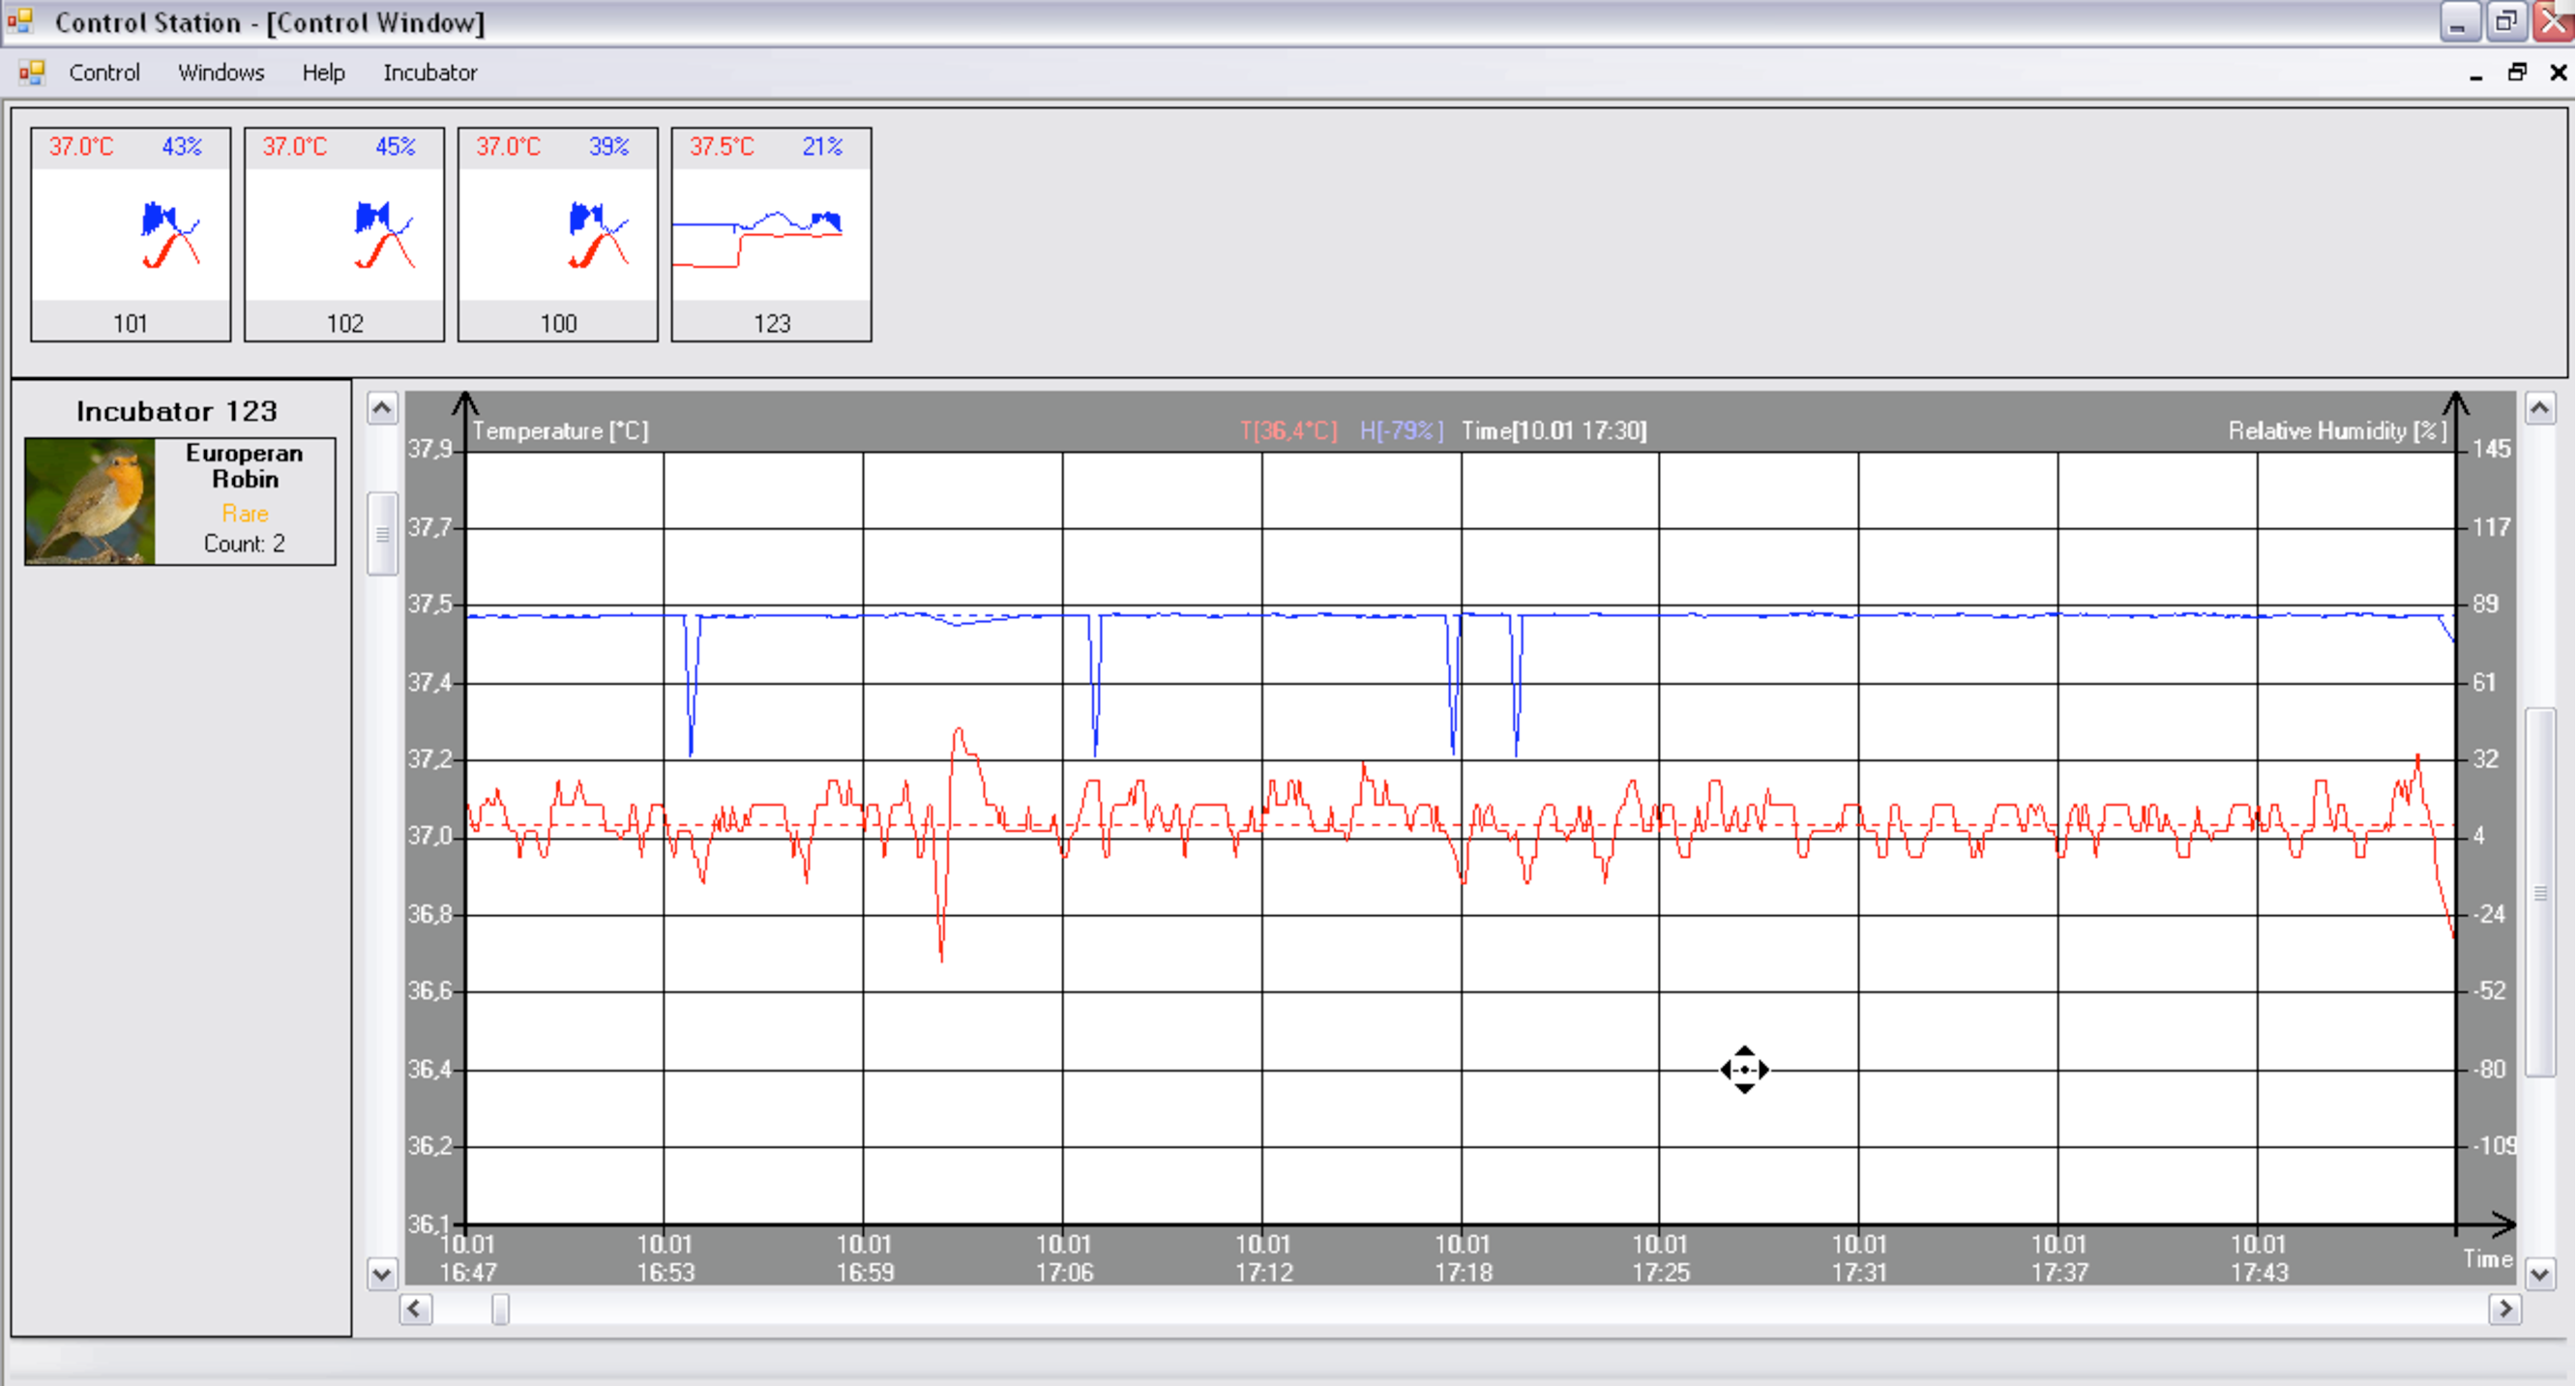
\includegraphics[width=\textwidth]{figures/Control}
\caption{Okno kontroli}\label{rys:Control}
\end{figure}

\begin{figure}[p] 
\centering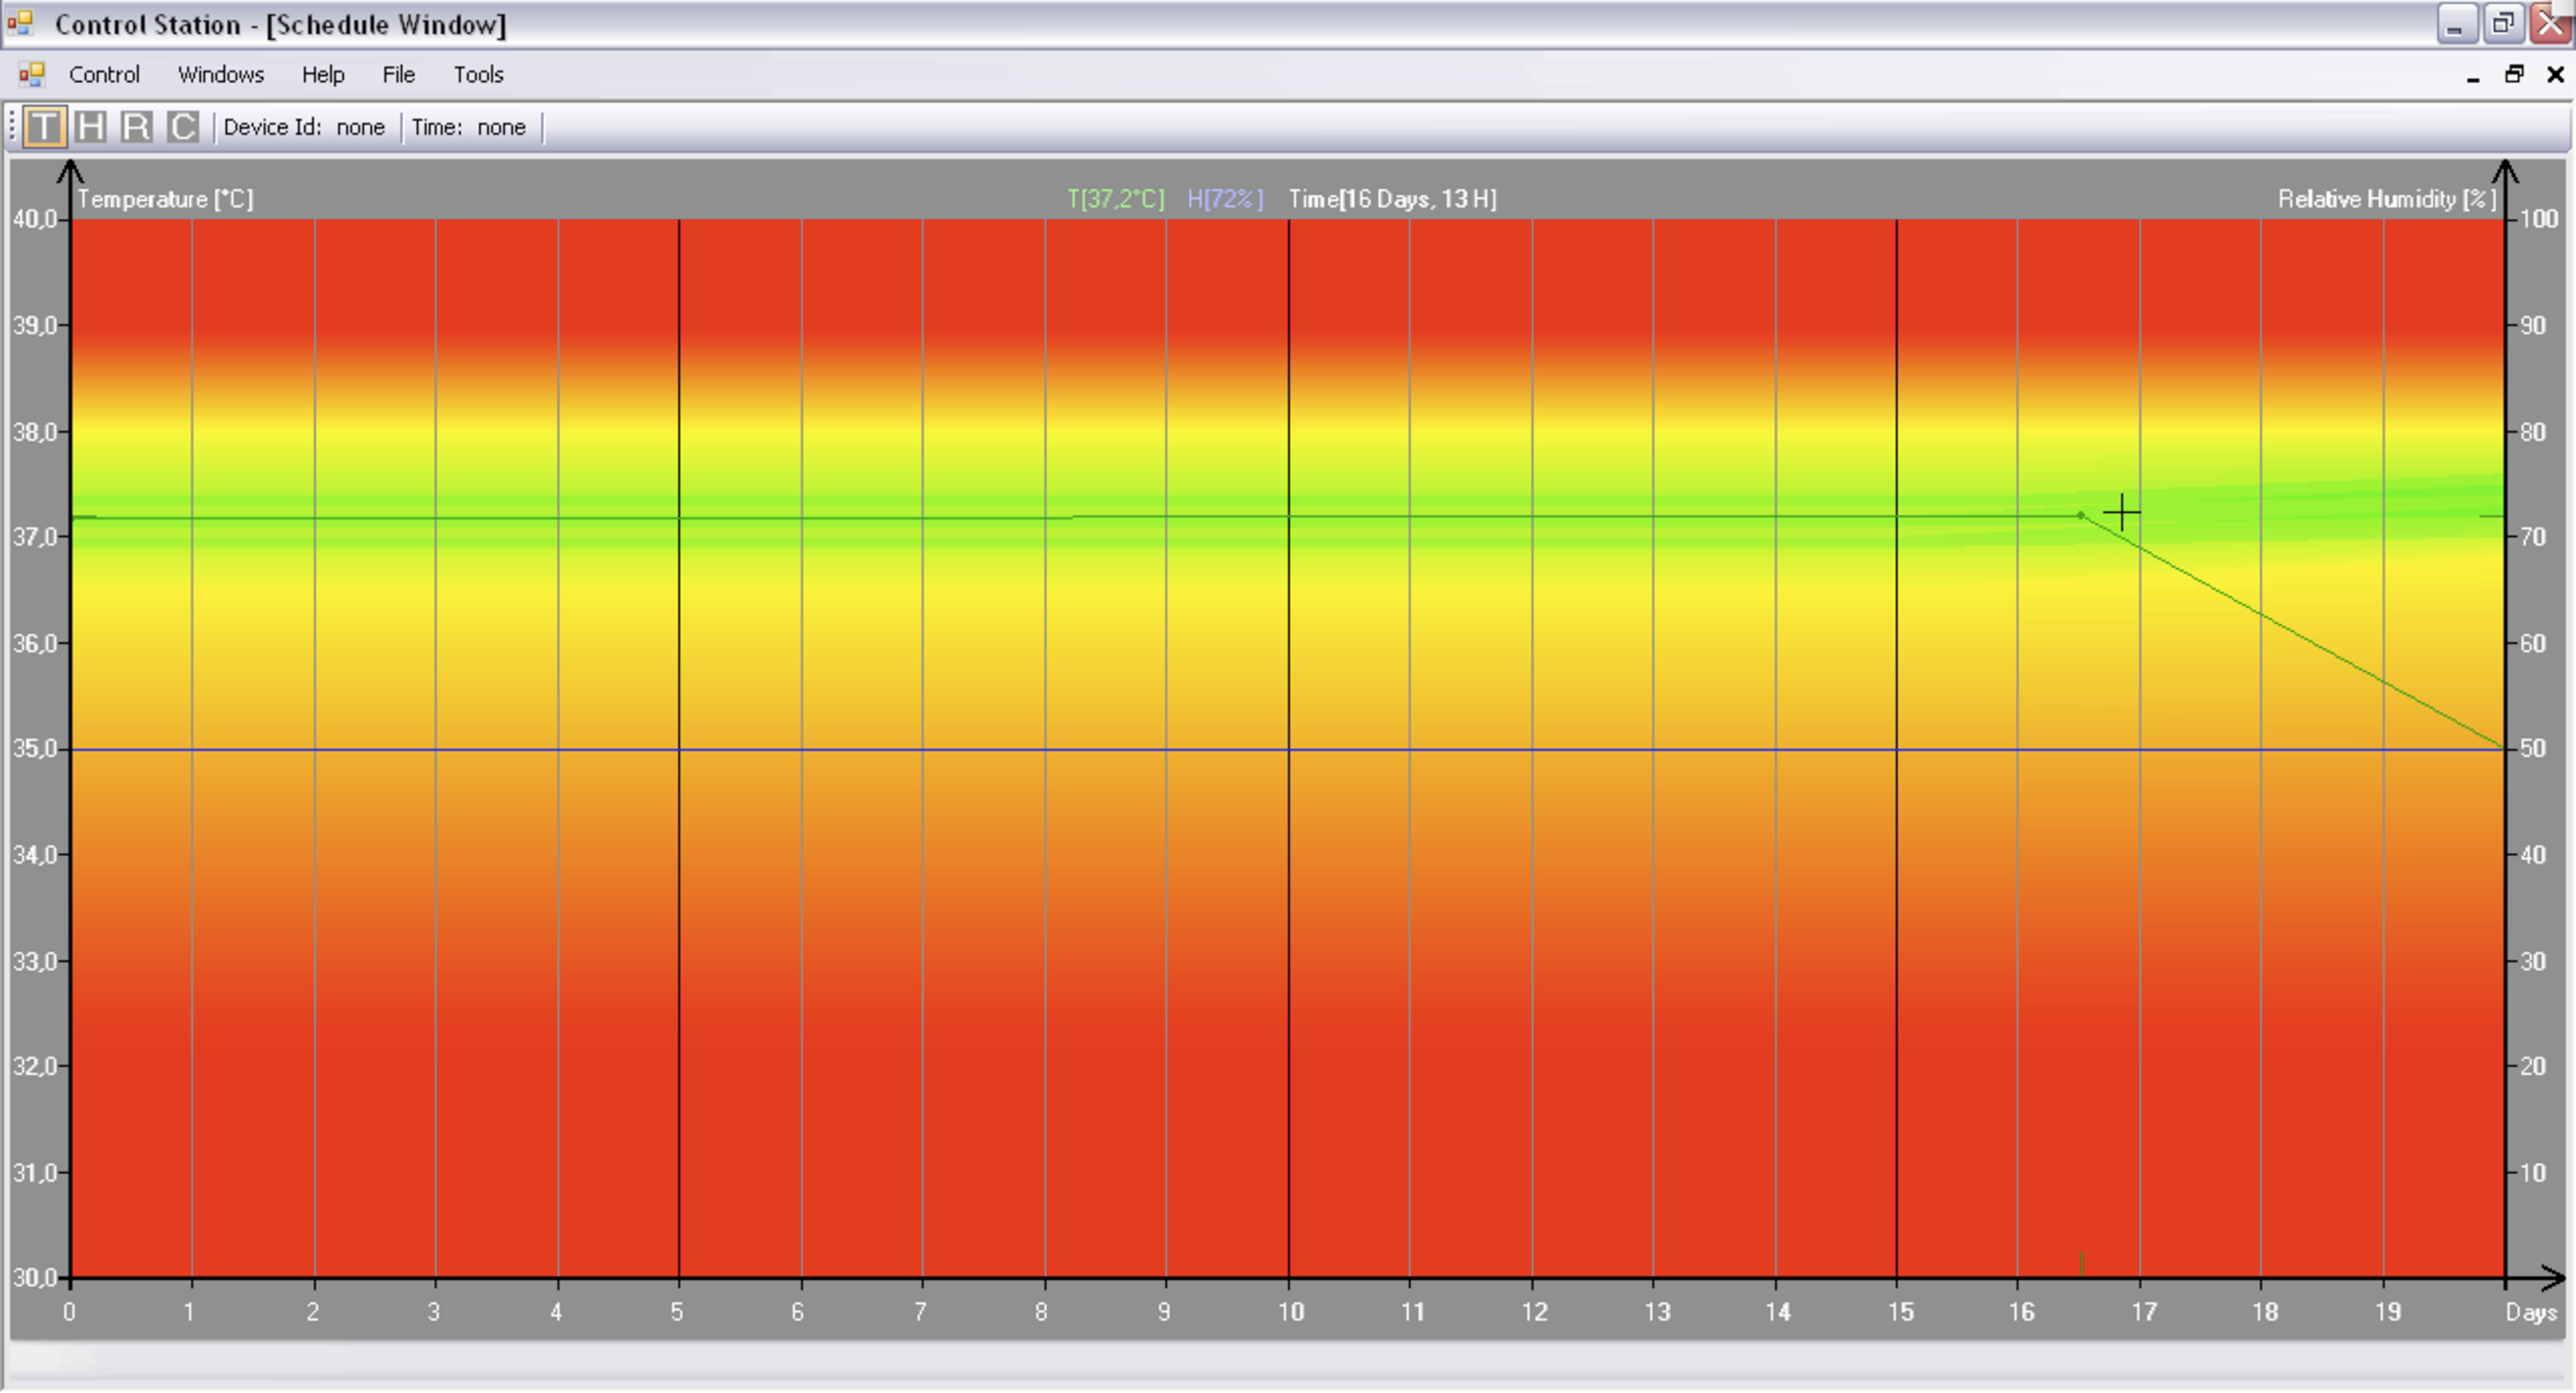
\includegraphics[width=\textwidth]{figures/Schedule}
\caption{Okno Planu Inkubacji z~nałożonymi na siebie wzorcami inkubacji trzech różnych gatunków}\label{rys:Schedule}
\end{figure}

\subsection{Interfejs programowania}
Po wyborze w~menu opcji ,,Schedule'' (Plan inkubacji) wyświetlane jest okno
programowania (ScheduleWindow) przedstawione na rysunku~\ref{rys:Schedule}. Okno
to służy do ustalenia pożądanych wartości sterowanych parametrów inkubacji. Na
pasku narzędzi do wyboru jest temperatura, wilgotność oraz częstość obracania
i~chłodzenia. Ustalanie przebiegu funkcji sterowanych parametrów odbywa się
podobnie jak w~inkubatorze przez dobór punktów (czas, wartość) przez które ma
przebiegać zadana funkcja. Użytkownik może też określić gatunki ptaków, których
jaja chce inkubować, wybierając z~menu opcję ,,Tools'' (Narzędzia) $\rightarrow$
,,Species'' (Gatunki). Okno dialogowe wyboru gatunków przedstawione jest na
rysunku~\ref{rys:Species}. Po wyborze gatunków w~tle wykresu pojawiają się
nałożone na siebie wzorce inkubacji wybranych gatunków. Mają one postać
gradientu koloru od czerwonego (dla zbyt wysokich wartości), poprzez zielony
(dla optymalnych wartości) do czerwonego (dla zbyt niskich wartości ustalanej
funkcji). Użytkownik powinien tak ustalać przebieg funkcji by znajdowała się ona
w obszarze optymalnym. Na wspomnianym rysunku~\ref{rys:Schedule} nałożone są
wzorce temperatury dla trzech różnych gatunków. Jak widać obszary optymalne dla
wybranych gatunków przesunięte są względem siebie o~około~0,2\st. Zielona
pozioma kreska przedstawia przebieg funkcji temperatury, dobrany tak by
minimalizować łączny błąd nastaw względem wzorca. Po ustaleniu wszystkich
parametrów plan inkubacji można przesłać do inkubatora. W~tym celu należy wybrać
w~menu opcję ,,Tools'' (Narzędzia) $\rightarrow$ ,,Send schedule'' (Prześlij
plan inkubacji). Pojawia się wówczas okno dialogowe
(rysunek~\ref{rys:SendSchedule}), w~którym użytkownik wybiera identyfikator
inkubatora, który chce zaprogramować. Wybrany inkubator otrzymuje nowy plan
inkubacji i~od tej chwili zaczyna go realizować.

\begin{figure}[b]
	\centering
	\mbox{
		\subfigure[Wybór inkubowanych gatunków]{
			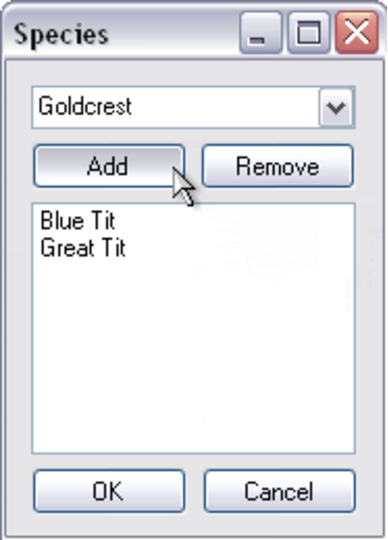
\includegraphics[width=0.3\textwidth]{figures/Species}
			\label{rys:Species}
		}
	\subfigure[Wysyłanie planu inkubacji do inkubatora]{
		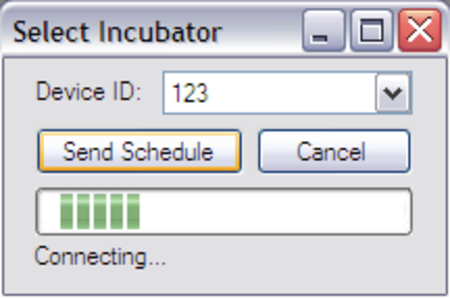
\includegraphics[width=0.3\textwidth]{figures/SendSchedule}
		\label{rys:SendSchedule}
		}
		\quad
		\subfigure[Pobieranie planu inkubacji od inkubatora]{
			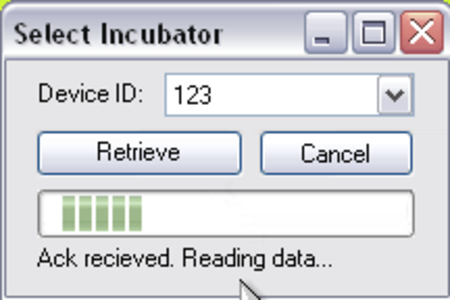
\includegraphics[width=0.3\textwidth]{figures/Retrieve}
			\label{rys:Retrieve}
		}
	}
	\caption{Okna dialogowe w~Stacji Kontrolnej}
	\label{rys:dialogi}
\end{figure}

Okno programowania (ScheduleWindow) pozwala też na pobranie z~inkubatora
aktualnego planu inkubacji. W~tym celu należy wybrać z~menu opcję ,,Tools''
(Narzędzia) $\rightarrow$ ,,Retrieve schedule'' (Pobierz plan inkubacji).
Podobnie jak przy wysyłaniu, w~oknie dialogowym (rysunek \ref{rys:Retrieve})
należy podać identyfikator inkubatora, z~którego ma być pobrany plan inkubacji.
Pobrany plan można dowolnie zmodyfikować i~przesłać z~powrotem do inkubatora.

\section{Centrum Nadzoru}

\subsection{Strona wstępu}
Na tej stronie użytkownik może zobaczyć informacje o~projekcie. Można tutaj
zamieścić informacje ułatwiające użytkownikowi korzystanie z~systemu
(\emph{FAQ} -- często zadawane pytania lub \emph{HOWTO} -- poradnik)
% tu bedzie obrazek

\subsection{Strona inkubacji}
Na tej stronie użytkownik może obejrzeć stan inkubacji (takiej, która się toczy
lub takiej która się zakończyła), którą może wybrać z~menu po lewej stronie.
W~górnej liście zakładek może zobaczyć informację odnośnie liczby inkubowanych
jaj lub wyklutych piskląt w~danej inkubacji. Na każdej zakładce dostępne są
informacje o~innym gatunku. W~dolnej liście zakładek użytkownik może zobaczyć
wykres reprezentujący stan zmiennych procesowych w~czasie. W~każdej zakładce
dostępne są informację o~innej zmiennej.
% tu bedzie obrazek

\subsection{Strona inkubatora}
Na tej stronie (rysunek~\ref{rys:CNinkubator}) użytkownik może przejrzeć stan inkubatorów w~jego grupie -- lista
dostępnych inkubatorów jest dostępna w~lewej części strony. Może również
ustawić czas, po którym zostanie do niego wysłany e-mail alarmujący,
gdy Centrum Nadzoru nie uzyska informacji o~stanie inkubatora.
% tu bedzie obrazek

\subsection{Strona gatunku}
Na tej stronie (rysunek~\ref{rys:CNgatunek}) użytkownik może zobaczyć obrazek przedstawiciela gatunku, krótką
informację oraz statystyki opisujące stan wiedzy systemu na temat tego gatunku
(np. ilość inkubacji, średnia klujność). Najciekawszą informacją na tej stronie
jest wzorzec inkubacji dla danego gatunku. Ze względów bezpieczeństwa użytkownik
nie może edytować stałych używanych przy generowaniu wzorców, może je jedynie obejrzeć.

\begin{figure}[p] 
\centering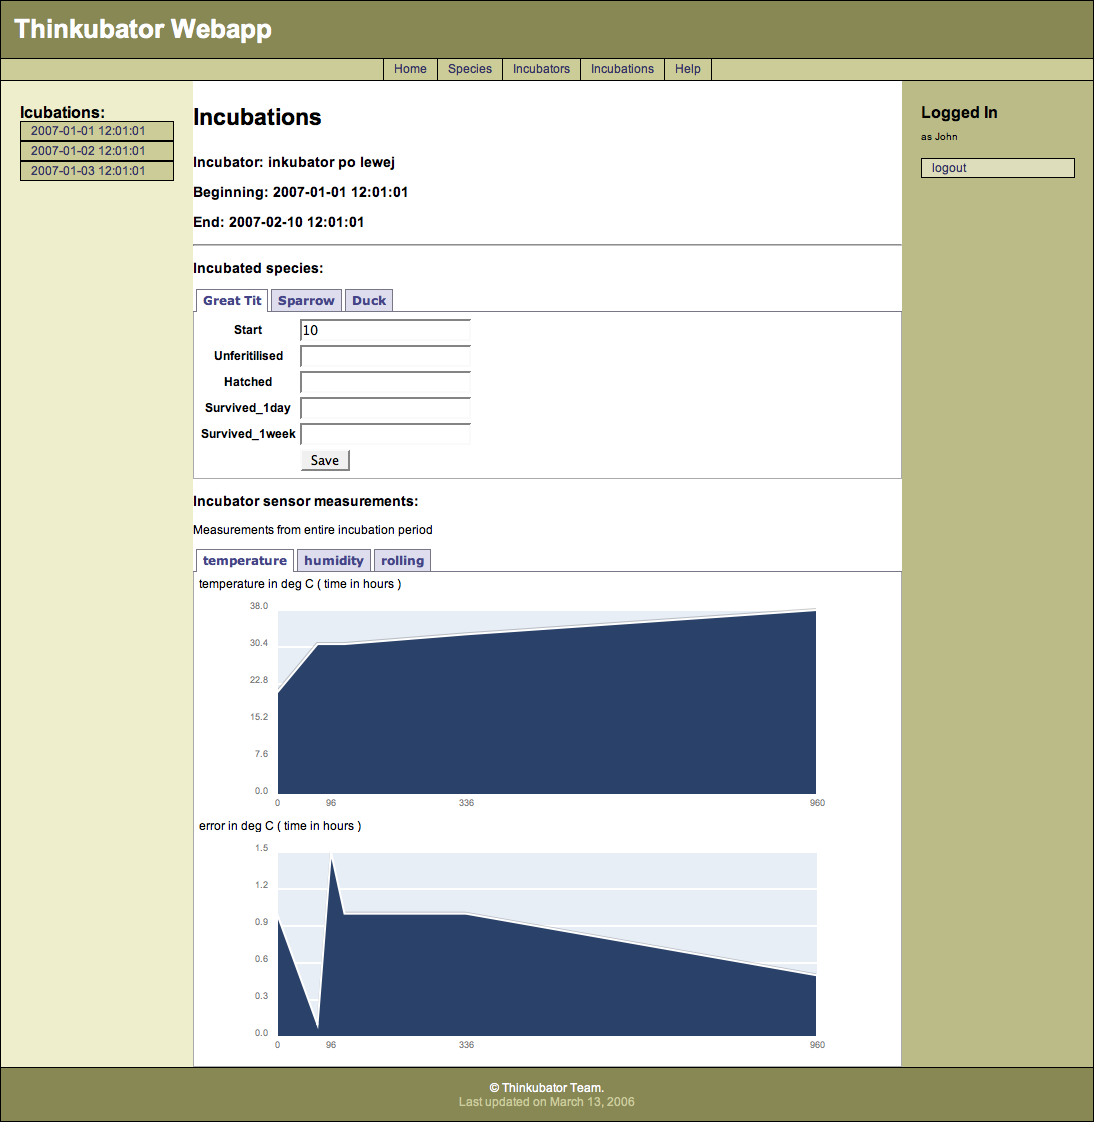
\includegraphics[width=.8\textwidth]{figures/CNinkubator}
\caption{Strona inkubatora}\label{rys:CNinkubator}
\end{figure}

\begin{figure}[p] 
\centering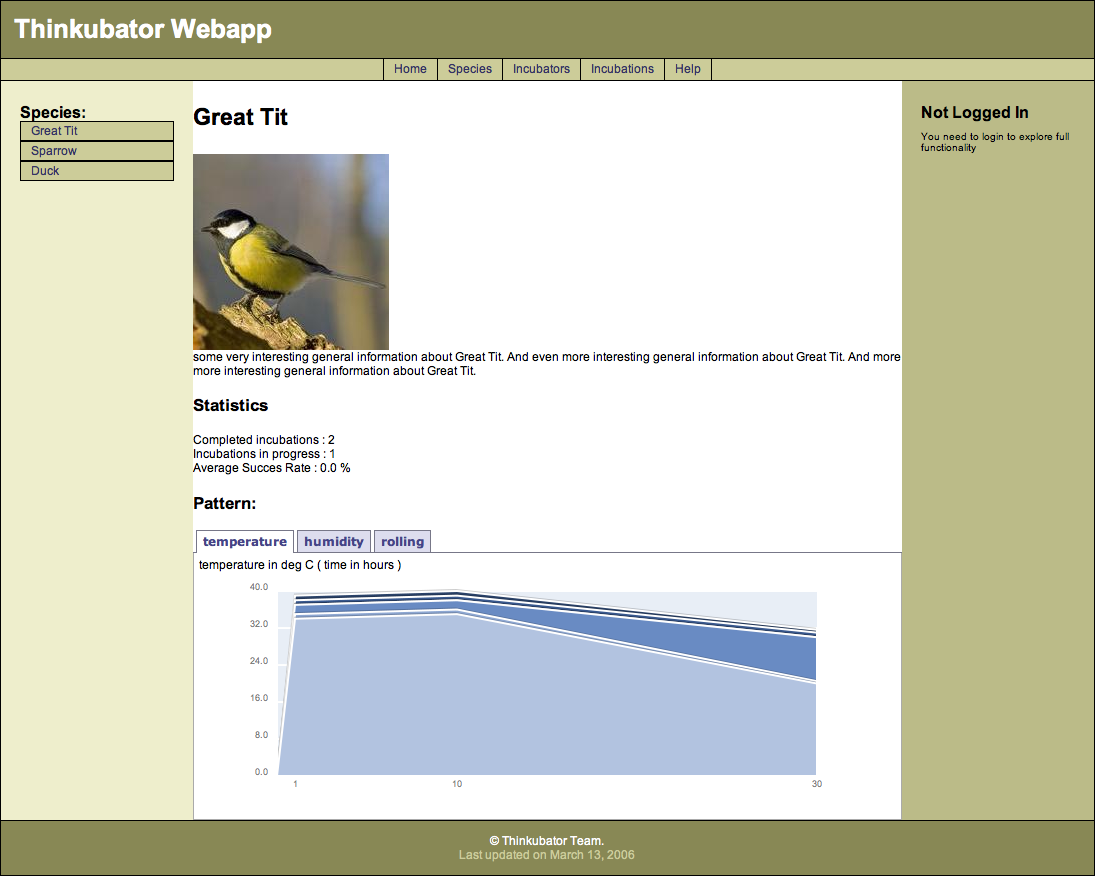
\includegraphics[width=.8\textwidth]{figures/CNgatunek}
\caption{Strona gatunku}\label{rys:CNgatunek}
\end{figure}

\subsection{Interfejs administracyjny}
Na tej stronie Administrator może bezpośrednio edytować zawartość bazy danych.
Dzięki temu ma on ułatwiony dostęp do jej zawartości i~może wygodnie edytować
wartości, które mają wpływ na globalną pracę systemu. Może on również poprawiać
błędy użytkowników.
% tu będzie obrazek



\chapter{Podsumowanie}
\label{sec:Podsumowanie}

\section{Stan Systemu}
Projekt zakończył się sukcesem, ponieważ w~trakcie pisania pracy był już w~pełni
funkcjonalny -- zaimplementowano wszystkie określone w~wymaganiach funkcje.
Pokonano wiele trudności z~dziedziny informatyki, automatyki oraz termodynamiki.
Uzyskano jakość sterowania temperaturą dorównującą lub nawet przekraczającą tą
w~obecnie stosowanych komercyjnie rozwiązaniach.  System Thinkubator umożliwia
rozproszoną wymianę danych oraz zdalne ustawianie urządzeń.  Użytkownik może
korzystać z~przyjaznego interfejsu podczas wykonywania tych trudnych czynności.
W~najbliższym czasie twórcy będą się konsultować z~przedstawicielami
Poznańskiego Nowego Zoo w~celu wdrożenia systemu oraz przeprowadzenia pierwszego
praktycznego testu -- próby wyklucia, który ostatecznie sprawdzi funkcjonalność
Thinkubatora.

\section{Dalszy Rozwój}
Głównym celem systemu Thinkubator jest ułatwienie pracy osobom zajmującym się
sztuczną inkubacją ptaków. Jego celem drugorzędnym jest wsparcie dla osób
zajmujących się badaniem tego procesu. W~tej chwili stworzony system jest
platformą umożliwiającą implementację zajmujących się tym rozszerzeń. Po
wdrożeniu, gdy tabele bazy danych Centrum Nadzoru wypełnią się informacjami
z~przeprowadzonych inkubacji oraz ich wynikami, możliwe będzie opracowanie
i~wdrożenie zaawansowanych algorytmów wyszukiwania wzorcowych przebiegów
procesu. Do tego celu potrzebne będą także konsultacje z~osobami zajmującymi się
badaniami nad inkubacją od strony biologicznej. 

Inną opcją systemu jest dostosowanie go do wylęgu gadów, płazów, owadów,
pajęczaków, gdzie również konieczna jest precyzyjna dobowa manipulacja
temperaturą. Podczas tworzenia systemu Thinkubator nie brano pod uwagę tych grup
zwierząt, jednak ze względu na wielkie możliwości stworzonego systemu, można go
będzie łatwo dostosować do wymogów inkubacji wymienionych gromad.  Zastosowanie
wymiennika ciepła pozwala stworzyć urządzenie przystosowane do każdego rodzaju
jaj, ponieważ nie jest on integralną częścią komory inkubacyjnej.
 
\section{Wnioski}
Realizacja projektu wymagała od twórców wiedzy z~bardzo wielu dziedzin szeroko
pojętej inżynierii. Podczas zbierania trudnych do zrozumienia wymagań konieczne
było poznania ornitologicznego żargonu. Z~kolei zastosowane rozwiązania
programistyczne były dobrane tak, aby twórcy mieli styczność z~najnowszymi
i~najciekawszymi narzędziami. Praca ze sprzętem wymagała dostosowywania
koncepcji do dostępnych zasobów oraz często zmieniającej się sytuacji (np.
awarie), a~praca w~czteroosobowym zespole wymagała sporej wiedzy z~dziedziny
zarządzania (nie tylko projektem informatycznym). Dzięki temu autorzy projektu
zyskali najcenniejszą rzecz -- doświadczenie.  



% All appendices and extra material, if you have any.
\cleardoublepage\appendix%

% Bibliography (books, articles) starts here.
\bibliographystyle{plalpha}{\raggedright\sloppy\small\bibliography{bibliography}}

% Colophon is a place where you should let others know about copyrights etc.
\ppcolophon
\end{document}
